\documentclass[11pt,a4paper]{article}
\usepackage[utf8]{inputenc}
\usepackage[margin=0.75in,footskip=0.25in]{geometry}

%\usepackage[francais]{babel}
\usepackage[T1]{fontenc}
\usepackage{amsmath}
\usepackage{amsfonts}
\usepackage{amssymb}
\usepackage{graphicx}
\graphicspath{{/home/utilisateur1/Documents/Genie_physique/H2018/Projet_II/Magnetisme_projet}}%changer le numéro du devoir
\usepackage{standalone}
\usepackage{tikz}
\renewcommand{\thesection}{\arabic{section}}
\author{Bastien Gauthier-Soumis,\\
 Edward Halle-Hannan, 1843683,\\
Massine Kadi, ,\\
Félix Pelletier, }
\title{Intention_de_projet_main}

\begin{document}
\begin{titlepage}
	\begin{flushright}
\def\logoscale{0.5}

\documentclass{standalone}
\usepackage{standalone}
\usepackage[utf8]{inputenc}
\usepackage{tikz}

\def\logoscale{1}
\begin{document}
\definecolor{c231f20}{RGB}{35,31,32}
\definecolor{ca7a5a6}{RGB}{167,165,166}


\begin{tikzpicture}[y=0.80pt, x=0.80pt, scale=\logoscale, yscale=-1.000000, xscale=1.000000, inner sep=0pt, outer sep=0pt]
\begin{scope}[cm={{1.25,0.0,0.0,-1.25,(0.0,167.5375)}}]
  \begin{scope}[scale=0.100]
    \path[fill=c231f20,nonzero rule] (0.0000,1149.1700) -- (36.0664,1149.1700) ..
      controls (52.1680,1149.1700) and (60.8203,1145.7300) .. (66.6211,1140.5200) ..
      controls (73.4688,1134.4100) and (76.6094,1125.6100) .. (76.6094,1114.7300) ..
      controls (76.6094,1097.7500) and (67.2070,1089.6800) .. (62.3047,1086.7100) ..
      controls (54.4063,1081.9500) and (45.7539,1081.5000) .. (37.2578,1081.1900) --
      (24.1328,1080.7400) -- (24.1328,1039.7600) -- (-0.0000,1039.7600) --
      (-0.0000,1149.1700) -- cycle(24.1328,1099.0900) .. controls
      (35.6133,1099.0900) and (39.9414,1099.0900) .. (42.7656,1100.2800) .. controls
      (44.7188,1101.0100) and (51.5742,1104.3100) .. (51.5742,1115.4800) .. controls
      (51.5742,1126.0600) and (47.5391,1128.2900) .. (44.2695,1129.6300) .. controls
      (40.3906,1131.1400) and (38.5938,1131.1400) .. (24.1328,1131.1400) --
      (24.1328,1099.0900);
    \path[fill=c231f20,nonzero rule] (95.2344,1110.5600) .. controls
      (95.2344,1121.7400) and (97.1680,1132.4800) .. (104.7730,1140.8200) ..
      controls (111.6210,1148.4300) and (121.9260,1151.2700) .. (132.1950,1151.2700)
      .. controls (143.3790,1151.2700) and (153.6720,1148.5700) ..
      (160.9770,1140.6600) .. controls (167.0700,1134.1200) and (170.5080,1124.4100)
      .. (170.5080,1106.8300) -- (170.5080,1080.3100) .. controls
      (170.5080,1064.9500) and (167.9880,1055.1100) .. (161.1130,1047.6600) ..
      controls (152.0200,1037.8100) and (138.9140,1036.7700) .. (131.9020,1036.7700)
      .. controls (121.1600,1036.7700) and (103.5860,1040.6500) ..
      (98.0664,1059.1400) .. controls (95.6836,1066.8800) and (95.2344,1076.4300) ..
      (95.2344,1081.2000) -- (95.2344,1110.5600) -- cycle(119.6880,1076.2900) ..
      controls (119.6880,1064.7900) and (121.9260,1056.6000) .. (132.6370,1056.6000)
      .. controls (145.6130,1056.6000) and (145.6130,1068.6800) ..
      (145.6130,1076.2900) -- (145.6130,1114.2800) .. controls (145.6130,1121.8900)
      and (145.6130,1131.1400) .. (132.9380,1131.1400) .. controls
      (119.6880,1131.1400) and (119.6880,1118.6300) .. (119.6880,1114.2800) --
      (119.6880,1076.2900);
    \path[fill=c231f20,nonzero rule] (199.8830,1149.1700) -- (224.3360,1149.1700) --
      (224.3360,1060.1800) -- (272.4730,1060.1800) -- (272.4730,1039.7600) --
      (199.8830,1039.7600) -- (199.8830,1149.1700);
    \path[fill=c231f20,nonzero rule] (308.2890,1039.7600) -- (308.2890,1082.9900) --
      (273.6990,1149.1700) -- (299.4920,1149.1700) -- (313.3280,1121.8900) ..
      controls (314.3950,1119.8000) and (318.7230,1110.4200) .. (319.6090,1108.4800)
      -- (320.3440,1108.4800) .. controls (322.4410,1113.1000) and
      (322.8910,1113.8500) .. (326.6090,1121.6000) -- (339.8830,1149.1700) --
      (365.3590,1149.1700) -- (332.4220,1083.8900) -- (332.4220,1039.7600) --
      (308.2890,1039.7600);
    \path[fill=c231f20,nonzero rule] (458.4570,1149.1700) -- (458.4570,1129.1900) --
      (431.1720,1129.1900) -- (431.1720,1039.7600) -- (406.1450,1039.7600) --
      (406.1450,1129.1900) -- (378.2700,1129.1900) -- (378.2700,1149.1700) --
      (458.4570,1149.1700);
    \path[fill=c231f20,nonzero rule] (483.7890,1149.1700) -- (557.2730,1149.1700) --
      (557.2730,1129.1900) -- (507.6370,1129.1900) -- (507.6370,1105.9300) --
      (541.7770,1105.9300) -- (541.7770,1085.9600) -- (507.9490,1085.9600) --
      (507.9490,1060.1800) -- (560.7030,1060.1800) -- (560.7030,1039.7600) --
      (483.7890,1039.7600) -- (483.7890,1149.1700);
    \path[fill=c231f20,nonzero rule] (585.4610,1112.3500) .. controls
      (585.4610,1137.3800) and (598.8670,1151.5500) .. (624.3550,1151.5500) ..
      controls (630.9300,1151.5500) and (640.7700,1150.2100) .. (648.3670,1144.2500)
      .. controls (658.2030,1136.5000) and (659.3950,1123.0800) ..
      (659.6880,1114.2800) -- (635.6910,1114.2800) .. controls (635.5350,1119.6500)
      and (635.2340,1131.5800) .. (623.3130,1131.5800) .. controls
      (620.3320,1131.5800) and (616.5940,1130.3900) .. (614.2300,1128.1600) ..
      controls (610.3520,1124.5800) and (610.1950,1119.2000) .. (610.1950,1116.2300)
      -- (610.1950,1074.6400) .. controls (610.1950,1068.6800) and
      (610.1950,1057.2000) .. (623.4690,1057.2000) .. controls (633.3130,1057.2000)
      and (636.2890,1065.2400) .. (636.2890,1077.0200) -- (660.4220,1077.0200) ..
      controls (660.2730,1069.1300) and (660.1450,1068.2200) .. (659.3950,1063.6100)
      .. controls (658.4770,1059.2800) and (657.0120,1051.3800) ..
      (647.9100,1044.0800) .. controls (640.1560,1037.8100) and (628.8280,1036.7700)
      .. (624.0630,1036.7700) .. controls (611.3870,1036.7700) and
      (602.5980,1039.7600) .. (595.7420,1046.4700) .. controls (591.2700,1050.7900)
      and (585.4610,1057.0400) .. (585.4610,1079.4100) -- (585.4610,1112.3500);
    \path[fill=c231f20,nonzero rule] (691.7460,1149.1700) -- (716.0470,1149.1700) --
      (716.0470,1107.7300) -- (746.7460,1107.7300) -- (746.7460,1149.1700) --
      (771.3550,1149.1700) -- (771.3550,1039.7600) -- (747.1880,1039.7600) --
      (747.1880,1087.0100) -- (716.1910,1087.0100) -- (716.1910,1039.7600) --
      (691.7460,1039.7600) -- (691.7460,1149.1700);
    \path[fill=c231f20,nonzero rule] (804.1600,1149.1700) -- (827.1020,1149.1700) --
      (855.2660,1098.0300) .. controls (856.4650,1095.8000) and (857.9610,1092.8300)
      .. (859.0040,1090.5900) .. controls (859.4340,1089.6800) and
      (860.9450,1085.6600) .. (861.3790,1084.9200) -- (862.1410,1084.9200) --
      (861.5550,1095.9600) .. controls (861.1050,1103.4000) and (861.1050,1104.3100)
      .. (861.1050,1108.4700) -- (861.1050,1149.1700) -- (883.1520,1149.1700) --
      (883.1520,1039.7600) -- (863.4770,1039.7600) -- (834.4020,1092.8300) ..
      controls (832.0200,1097.1400) and (831.8870,1097.5900) .. (826.2230,1110.8700)
      -- (825.4690,1110.8700) .. controls (825.6130,1107.7300) and
      (826.2230,1093.8700) .. (826.2230,1091.0300) -- (826.2230,1039.7600) --
      (804.1600,1039.7600) -- (804.1600,1149.1700);
    \path[fill=c231f20,nonzero rule] (911.9340,1039.7600) -- (911.9340,1049.4500) --
      (924.7460,1049.4500) -- (924.7460,1139.6300) -- (911.9340,1139.6300) --
      (911.9340,1149.1700) -- (961.8550,1149.1700) -- (961.8550,1139.6300) --
      (948.8950,1139.6300) -- (948.8950,1049.7400) -- (961.8550,1049.7400) --
      (961.8550,1039.7600) -- (911.9340,1039.7600);
    \path[fill=c231f20,nonzero rule] (1068.5900,1029.6300) .. controls
      (1064.2800,1029.6300) and (1061.2900,1029.6300) .. (1056.5200,1031.8500) ..
      controls (1049.8200,1035.1300) and (1046.9900,1039.7600) ..
      (1045.9300,1043.1800) .. controls (1037.5800,1037.5200) and
      (1027.7600,1036.7700) .. (1022.0900,1036.7700) .. controls
      (1011.3600,1036.7700) and (993.7770,1040.6500) .. (988.2540,1059.1300) ..
      controls (985.8790,1066.8800) and (985.4380,1076.4400) .. (985.4380,1081.1900)
      -- (985.4380,1110.5500) .. controls (985.4380,1121.7400) and
      (987.3550,1132.4800) .. (994.9610,1140.8200) .. controls (1001.8100,1148.4300)
      and (1012.0900,1151.2600) .. (1022.3900,1151.2600) .. controls
      (1033.5600,1151.2600) and (1043.8600,1148.5700) .. (1051.1600,1140.6800) ..
      controls (1057.2800,1134.1200) and (1060.6900,1124.4300) ..
      (1060.6900,1106.8400) -- (1060.6900,1080.3000) .. controls
      (1060.6900,1071.2100) and (1059.7900,1063.9100) .. (1057.5700,1058.2400) ..
      controls (1061.5900,1053.1800) and (1064.1200,1053.1800) ..
      (1068.5900,1053.1800) -- (1068.5900,1029.6300) -- cycle(1022.3900,1089.8400)
      .. controls (1028.5000,1088.9400) and (1031.1800,1087.3000) ..
      (1033.8700,1084.0300) .. controls (1034.4500,1083.2800) and
      (1034.9100,1082.7000) .. (1035.8000,1081.1900) -- (1035.8000,1114.2900) ..
      controls (1035.8000,1122.3400) and (1035.3400,1131.1400) ..
      (1022.8300,1131.1400) .. controls (1009.8700,1131.1400) and
      (1009.8700,1118.1600) .. (1009.8700,1114.2900) -- (1009.8700,1076.2700) ..
      controls (1009.8700,1064.5000) and (1012.2700,1056.6000) ..
      (1022.9800,1056.6000) .. controls (1027.6100,1056.6000) and
      (1030.5800,1058.2400) .. (1032.5300,1060.9300) .. controls
      (1029.1000,1066.4400) and (1027.3100,1067.9300) .. (1022.3900,1069.4300) --
      (1022.3900,1089.8400);
    \path[fill=c231f20,nonzero rule] (1095.0100,1149.1700) -- (1119.9000,1149.1700)
      -- (1119.9000,1077.0300) .. controls (1119.9000,1070.4800) and
      (1119.9000,1056.9100) .. (1134.6500,1056.9100) .. controls
      (1139.2800,1056.9100) and (1150.0100,1056.9100) .. (1150.0100,1076.8800) --
      (1150.0100,1149.1700) -- (1174.3100,1149.1700) -- (1174.3100,1076.7300) ..
      controls (1174.3100,1070.1600) and (1174.1700,1054.3700) ..
      (1162.9900,1045.2800) .. controls (1155.3800,1039.1600) and
      (1145.9900,1036.9300) .. (1136.0000,1036.9300) .. controls
      (1124.5200,1036.9300) and (1112.7500,1039.7600) .. (1106.0200,1046.0200) ..
      controls (1095.4500,1056.0100) and (1095.0100,1068.5300) ..
      (1095.0100,1078.3600) -- (1095.0100,1149.1700);
    \path[fill=c231f20,nonzero rule] (1205.4500,1149.1700) -- (1278.9400,1149.1700)
      -- (1278.9400,1129.1900) -- (1229.3100,1129.1900) -- (1229.3100,1105.9300) --
      (1263.4500,1105.9300) -- (1263.4500,1085.9600) -- (1229.5900,1085.9600) --
      (1229.5900,1060.1800) -- (1282.3600,1060.1800) -- (1282.3600,1039.7600) --
      (1205.4500,1039.7600) -- (1205.4500,1149.1700);
    \path[fill=c231f20,nonzero rule] (433.3670,970.2850) -- (465.5660,970.2850) --
      (478.5230,924.6680) .. controls (479.8630,919.7420) and (480.4690,918.1020) ..
      (481.6600,913.1840) .. controls (482.2660,910.9530) and (484.4920,901.3980) ..
      (484.9490,899.4690) -- (485.6840,899.4690) .. controls (487.3130,908.5660) and
      (488.9650,915.4100) .. (491.6410,925.1130) -- (504.4530,970.2850) --
      (536.8090,970.2850) -- (536.8090,860.8590) -- (515.8010,860.8590) --
      (515.8010,919.7420) .. controls (515.8010,927.4840) and (516.4060,940.4770) ..
      (516.8360,950.8950) -- (516.2300,950.8950) -- (493.5740,860.8590) --
      (477.0510,860.8590) -- (453.7770,950.8950) -- (453.0350,950.8950) .. controls
      (453.1840,945.8320) and (454.0700,923.6250) .. (454.0700,919.0000) --
      (454.0700,860.8590) -- (433.3670,860.8590) -- (433.3670,970.2850);
    \path[fill=c231f20,nonzero rule] (566.3400,931.6600) .. controls
      (566.3400,942.8550) and (568.2810,953.5780) .. (575.8790,961.9260) .. controls
      (582.7420,969.5470) and (593.0200,972.3750) .. (603.3200,972.3750) .. controls
      (614.4920,972.3750) and (624.7850,969.6840) .. (632.0700,961.7810) .. controls
      (638.1840,955.2230) and (641.6090,945.5390) .. (641.6090,927.9410) --
      (641.6090,901.4060) .. controls (641.6090,886.0510) and (639.0820,876.2190) ..
      (632.2070,868.7730) .. controls (623.1250,858.9180) and (610.0200,857.8830) ..
      (603.0080,857.8830) .. controls (592.2580,857.8830) and (574.6880,861.7700) ..
      (569.1800,880.2460) .. controls (566.7850,887.9920) and (566.3400,897.5230) ..
      (566.3400,902.3050) -- (566.3400,931.6600) -- cycle(590.7930,897.3950) ..
      controls (590.7930,885.9100) and (593.0200,877.7070) .. (603.7620,877.7070) ..
      controls (616.7110,877.7070) and (616.7110,889.7850) .. (616.7110,897.3950) --
      (616.7110,935.3950) .. controls (616.7110,942.9840) and (616.7110,952.2420) ..
      (604.0550,952.2420) .. controls (590.7930,952.2420) and (590.7930,939.7300) ..
      (590.7930,935.3950) -- (590.7930,897.3950);
    \path[fill=c231f20,nonzero rule] (673.9650,970.2850) -- (696.9260,970.2850) --
      (725.1050,919.1410) .. controls (726.2890,916.9100) and (727.7730,913.9340) ..
      (728.8160,911.6990) .. controls (729.2770,910.7930) and (730.7540,906.7770) ..
      (731.1990,906.0310) -- (731.9410,906.0310) -- (731.3550,917.0660) .. controls
      (730.9180,924.5120) and (730.9180,925.4180) .. (730.9180,929.5860) --
      (730.9180,970.2850) -- (752.9880,970.2850) -- (752.9880,860.8590) --
      (733.2930,860.8590) -- (704.2380,913.9340) .. controls (701.8480,918.2580) and
      (701.6880,918.7030) .. (696.0350,931.9730) -- (695.2810,931.9730) .. controls
      (695.4300,928.8360) and (696.0350,914.9690) .. (696.0350,912.1450) --
      (696.0350,860.8590) -- (673.9650,860.8590) -- (673.9650,970.2850);
    \path[fill=c231f20,nonzero rule] (861.9530,970.2850) -- (861.9530,950.3010) --
      (834.6800,950.3010) -- (834.6800,860.8590) -- (809.6290,860.8590) --
      (809.6290,950.3010) -- (781.7460,950.3010) -- (781.7460,970.2850) --
      (861.9530,970.2850);
    \path[fill=c231f20,nonzero rule] (912.7730,860.8590) -- (889.0630,860.8590) --
      (889.0630,970.2850) -- (924.4020,970.2850) .. controls (942.1410,970.2850) and
      (964.6560,967.8910) .. (964.6560,938.5430) .. controls (964.6560,924.6600) and
      (959.1410,914.0900) .. (943.7890,909.4610) -- (967.6450,860.8590) --
      (941.5550,860.8590) -- (920.8280,905.5700) -- (912.7730,905.5700) --
      (912.7730,860.8590) -- cycle(912.7730,923.0270) .. controls
      (926.3400,923.0270) and (928.4300,923.0270) .. (931.8750,924.2270) .. controls
      (939.4730,926.8910) and (940.0590,932.8630) .. (940.0590,938.8200) .. controls
      (940.0590,946.4340) and (937.6760,950.1450) .. (932.8980,951.9340) .. controls
      (929.1800,953.2770) and (926.1990,953.2770) .. (912.7730,953.2770) --
      (912.7730,923.0270);
    \path[fill=c231f20,nonzero rule] (994.7730,970.2850) -- (1068.2600,970.2850) --
      (1068.2600,950.3010) -- (1018.6200,950.3010) -- (1018.6200,927.0510) --
      (1052.7500,927.0510) -- (1052.7500,907.0700) -- (1018.9200,907.0700) --
      (1018.9200,881.3010) -- (1071.6900,881.3010) -- (1071.6900,860.8590) --
      (994.7730,860.8590) -- (994.7730,970.2850) -- cycle(1054.4000,1001.2800) --
      (1032.3500,979.6800) -- (1017.2700,979.6800) -- (1031.2900,1001.2800) --
      (1054.4000,1001.2800);
    \path[fill=c231f20,nonzero rule] (1153.9800,970.2850) -- (1185.5800,860.8590) --
      (1162.1800,860.8590) -- (1156.6700,882.6330) -- (1123.1300,882.6330) --
      (1117.4700,860.8590) -- (1094.0600,860.8590) -- (1124.9100,970.2850) --
      (1153.9800,970.2850) -- cycle(1139.8200,950.7420) -- (1139.2200,950.7420) --
      (1127.3000,901.2620) -- (1151.8800,901.2620) -- (1139.8200,950.7420);
    \path[fill=c231f20,nonzero rule] (1209.7400,970.2850) -- (1234.1900,970.2850) --
      (1234.1900,881.3010) -- (1282.3400,881.3010) -- (1282.3400,860.8590) --
      (1209.7400,860.8590) -- (1209.7400,970.2850);
    \path[fill=c231f20,nonzero rule] (1881.9200,958.1020) .. controls
      (1881.8700,958.2030) and (1881.5800,958.2190) .. (1881.5000,958.1250) ..
      controls (1879.8200,956.2230) and (1877.3200,954.3750) .. (1873.9800,954.3590)
      .. controls (1875.6800,950.3050) and (1877.0700,945.1760) ..
      (1877.0700,939.7190) .. controls (1877.0700,934.2270) and (1876.3800,925.9960)
      .. (1874.0600,920.5700) .. controls (1877.8300,920.8630) and
      (1881.6000,920.9960) .. (1881.6000,920.9960) .. controls (1881.6000,920.9960)
      and (1884.9900,920.8910) .. (1889.3500,920.5660) .. controls
      (1887.0500,925.9880) and (1886.3900,934.2270) .. (1886.3900,939.6990) ..
      controls (1886.3900,945.1600) and (1887.7400,950.3050) .. (1889.4500,954.3590)
      .. controls (1886.1200,954.3590) and (1883.5900,956.1910) ..
      (1881.9200,958.1020);
    \path[fill=c231f20,nonzero rule] (1846.4100,982.2460) .. controls
      (1853.0500,978.2850) and (1859.1500,974.2150) .. (1863.5200,966.8980) ..
      controls (1861.5200,966.0860) and (1859.4300,965.1910) .. (1857.2500,964.0980)
      .. controls (1836.6800,953.9730) and (1840.8400,918.5780) ..
      (1858.9700,918.0820) .. controls (1861.3600,918.4730) and (1863.9800,918.8440)
      .. (1866.5600,919.1020) .. controls (1868.8100,923.3550) and
      (1870.2500,928.0390) .. (1871.0400,932.7150) .. controls (1869.6700,930.1840)
      and (1867.4600,928.5310) .. (1864.9800,928.5310) .. controls
      (1860.7900,928.5310) and (1857.4300,933.1840) .. (1857.4300,938.9490) ..
      controls (1857.4300,944.7150) and (1860.7900,949.3710) .. (1864.9800,949.3710)
      .. controls (1867.8700,949.3710) and (1870.3800,947.1450) ..
      (1871.6300,943.8870) .. controls (1871.3300,949.5000) and (1869.9900,954.5740)
      .. (1867.8700,958.3090) .. controls (1867.5000,958.9610) and
      (1867.5600,959.7810) .. (1868.0300,960.3630) .. controls (1868.5000,960.9410)
      and (1869.3000,961.1720) .. (1870.0100,960.9410) .. controls
      (1876.3600,958.8240) and (1880.2500,965.2700) .. (1880.4500,965.5430) ..
      controls (1880.7000,966.0080) and (1881.0700,966.3830) .. (1881.6800,966.3830)
      .. controls (1882.2700,966.3830) and (1882.7000,966.0350) ..
      (1883.0000,965.5160) .. controls (1883.1800,965.2700) and (1887.0900,958.8130)
      .. (1893.4000,960.9260) .. controls (1894.1200,961.1680) and
      (1894.9300,960.9410) .. (1895.3900,960.3550) .. controls (1895.8600,959.7770)
      and (1895.9300,958.9610) .. (1895.5700,958.2930) .. controls
      (1893.4400,954.5630) and (1892.1100,949.4840) .. (1891.7800,943.8750) ..
      controls (1893.0500,947.1450) and (1895.5700,949.3550) .. (1898.4600,949.3550)
      .. controls (1902.6000,949.3550) and (1906.0200,944.6840) ..
      (1906.0200,938.9380) .. controls (1906.0200,933.1840) and (1902.6000,928.5310)
      .. (1898.4600,928.5310) .. controls (1895.9700,928.5310) and
      (1893.7600,930.1720) .. (1892.4000,932.7150) .. controls (1893.1800,928.0160)
      and (1894.6300,923.3480) .. (1896.8800,919.1020) .. controls
      (1899.4500,918.8280) and (1902.0700,918.4730) .. (1904.4600,918.0550) ..
      controls (1922.6000,918.5740) and (1926.7700,953.9730) .. (1906.2000,964.0820)
      .. controls (1903.9800,965.1720) and (1901.8900,966.0660) ..
      (1899.9000,966.8870) .. controls (1904.2600,974.1990) and (1910.3700,978.2730)
      .. (1917.0100,982.2270) .. controls (1924.5300,986.6950) and
      (1931.0500,990.8400) .. (1936.2700,999.4490) .. controls (1936.7800,1000.3100)
      and (1936.5100,1001.4100) .. (1935.6600,1001.9300) .. controls
      (1934.8000,1002.4600) and (1933.6900,1002.1900) .. (1933.1600,1001.3400) ..
      controls (1928.4100,993.5270) and (1921.6600,989.8160) .. (1914.7300,985.7380)
      .. controls (1907.6800,981.5940) and (1900.1400,977.4800) ..
      (1895.2400,968.7340) .. controls (1889.7900,970.8910) and (1885.3700,972.8670)
      .. (1882.0100,977.1290) .. controls (1881.8700,977.2810) and
      (1881.6000,977.3440) .. (1881.4600,977.1450) .. controls (1878.0700,972.8910)
      and (1873.6400,970.9100) .. (1868.1900,968.7500) .. controls
      (1863.3200,977.4920) and (1855.7600,981.6050) .. (1848.7000,985.7700) ..
      controls (1841.7900,989.8160) and (1835.0400,993.5430) ..
      (1830.2800,1001.3400) .. controls (1829.7600,1002.1900) and
      (1828.6400,1002.4800) .. (1827.7700,1001.9600) .. controls
      (1826.9100,1001.4500) and (1826.6400,1000.3100) .. (1827.1700,999.4490) ..
      controls (1832.4000,990.8710) and (1838.8900,986.7150) ..
      (1846.4100,982.2460);
    \path[fill=c231f20,nonzero rule] (1973.5700,829.3440) .. controls
      (1990.3200,818.1800) and (2007.5300,809.1720) .. (2023.8900,790.3790) ..
      controls (2038.3700,773.7850) and (2041.6500,764.7460) .. (2041.6500,759.9410)
      .. controls (2041.6500,758.5470) and (2041.3700,757.5230) ..
      (2041.0100,756.7770) .. controls (2038.8200,752.1800) and (2031.0200,751.4960)
      .. (2024.8600,751.7030) .. controls (2021.9500,751.8090) and
      (2019.2200,751.9690) .. (2016.5400,752.1480) .. controls (2013.8300,763.5270)
      and (2003.7500,787.8240) .. (1978.7900,809.5120) .. controls
      (1978.5000,809.7850) and (1978.0500,809.7850) .. (1977.7800,809.5080) ..
      controls (1977.5000,809.2150) and (1977.5400,808.7700) .. (1977.7900,808.4730)
      .. controls (1998.9200,785.4380) and (2008.0600,763.7660) ..
      (2010.6900,752.6290) .. controls (1986.2300,754.9960) and (1971.7400,761.1050)
      .. (1968.5900,770.5430) .. controls (1968.5200,770.7540) and
      (1968.4200,770.9490) .. (1968.3000,771.1170) .. controls (1963.4000,790.6170)
      and (1950.9000,814.9530) .. (1937.5300,828.3750) .. controls
      (1937.2500,828.6800) and (1936.8000,828.6880) .. (1936.5200,828.4300) ..
      controls (1936.2300,828.1560) and (1936.2100,827.6910) .. (1936.4800,827.3830)
      .. controls (1946.8300,815.3520) and (1957.6000,791.8950) ..
      (1962.5200,772.7540) .. controls (1935.1600,776.5350) and (1927.1700,789.5820)
      .. (1920.3800,804.9530) .. controls (1914.9200,817.3360) and
      (1913.6100,828.3590) .. (1913.6100,838.8130) .. controls (1913.6100,843.5350)
      and (1913.8800,848.1480) .. (1914.1600,852.6990) .. controls
      (1914.4000,857.2230) and (1914.6500,861.8320) .. (1914.6500,866.5040) ..
      controls (1914.6500,868.8830) and (1914.3600,873.5430) .. (1914.1000,877.5350)
      .. controls (1936.7200,850.6720) and (1954.2400,842.2150) ..
      (1973.5700,829.3440) -- cycle(1910.2700,710.5780) .. controls
      (1891.4400,709.1330) and (1872.0500,709.0940) .. (1853.4200,710.5080) ..
      controls (1851.2300,714.6990) and (1849.0200,719.4690) .. (1846.9300,724.8130)
      .. controls (1868.0700,722.4300) and (1895.1600,722.5630) ..
      (1916.7200,724.8830) .. controls (1914.6500,719.5350) and (1912.4400,714.7660)
      .. (1910.2700,710.5780) -- cycle(1881.8100,678.3520) .. controls
      (1879.5600,678.3520) and (1871.3500,683.0000) .. (1861.5800,696.9730) ..
      controls (1873.8900,696.3980) and (1889.7500,696.4380) .. (1902.1300,697.0430)
      .. controls (1892.3600,683.0200) and (1884.0600,678.3520) ..
      (1881.8100,678.3520) -- cycle(1752.7400,752.6480) .. controls
      (1755.3900,763.7700) and (1764.5300,785.4450) .. (1785.6300,808.4730) ..
      controls (1785.9100,808.7700) and (1785.9300,809.2150) .. (1785.6600,809.5120)
      .. controls (1785.3500,809.8050) and (1784.9300,809.8050) ..
      (1784.6100,809.5350) .. controls (1759.7100,787.8320) and (1749.6000,763.5860)
      .. (1746.9100,752.1680) .. controls (1744.2300,751.9880) and
      (1741.4700,751.8280) .. (1738.5700,751.7270) .. controls (1732.4200,751.4960)
      and (1724.6100,752.1800) .. (1722.4100,756.7810) .. controls
      (1722.0700,757.5350) and (1721.7800,758.5660) .. (1721.7800,759.9570) ..
      controls (1721.7800,764.7620) and (1725.0700,773.8010) .. (1739.5300,790.4100)
      .. controls (1755.9000,809.1880) and (1773.0900,818.1800) ..
      (1789.8600,829.3550) .. controls (1809.2100,842.2300) and (1826.7200,850.6800)
      .. (1849.3200,877.5390) .. controls (1849.0600,873.5430) and
      (1848.7500,868.8980) .. (1848.7500,866.5430) .. controls (1848.7500,861.8320)
      and (1849.0200,857.2300) .. (1849.2800,852.6990) .. controls
      (1849.5300,848.1480) and (1849.8000,843.5350) .. (1849.8000,838.8130) ..
      controls (1849.8000,828.3750) and (1848.5200,817.3360) .. (1843.0500,804.9530)
      .. controls (1836.2600,789.5820) and (1828.2800,776.5390) ..
      (1800.9200,772.7730) .. controls (1805.8600,791.9060) and (1816.6200,815.3710)
      .. (1826.9500,827.4140) .. controls (1827.2300,827.7110) and
      (1827.2300,828.1560) .. (1826.9100,828.4300) .. controls (1826.6200,828.7030)
      and (1826.1700,828.6800) .. (1825.9000,828.3790) .. controls
      (1812.4700,814.9340) and (1799.9800,790.5310) .. (1795.0900,771.0120) ..
      controls (1795.0000,770.8550) and (1794.9200,770.7150) .. (1794.8600,770.5470)
      .. controls (1791.7000,761.1170) and (1777.2100,755.0160) ..
      (1752.7400,752.6480) -- cycle(1924.5500,752.8520) .. controls
      (1923.6200,747.7850) and (1922.5100,743.0080) .. (1921.2500,738.5160) ..
      controls (1895.4900,735.1370) and (1867.7200,735.1450) .. (1842.4000,738.4300)
      .. controls (1841.1400,742.9410) and (1840.0100,747.7500) ..
      (1839.0800,752.8550) .. controls (1865.3700,748.7030) and (1897.4700,748.9570)
      .. (1924.5500,752.8520) -- cycle(1837.2900,765.8980) .. controls
      (1836.8400,770.5980) and (1836.5600,775.4880) .. (1836.5000,780.5940) ..
      controls (1863.2200,775.4410) and (1899.5600,775.7420) .. (1927.1300,780.5630)
      .. controls (1927.0700,775.5080) and (1926.8000,770.6560) ..
      (1926.3500,765.9920) .. controls (1897.4400,761.6520) and (1865.6300,761.6520)
      .. (1837.2900,765.8980) -- cycle(1881.5000,807.9220) .. controls
      (1891.9900,807.9180) and (1901.8600,807.5700) .. (1910.8000,806.8950) --
      (1914.3100,806.4060) .. controls (1914.7700,805.2460) and (1915.2100,804.0820)
      .. (1915.7400,802.8950) .. controls (1917.2300,799.5040) and
      (1918.8300,796.1840) .. (1920.6400,792.9920) .. controls (1894.2100,788.7110)
      and (1868.6300,788.7070) .. (1842.6900,792.8520) .. controls
      (1844.5600,796.0780) and (1846.1700,799.4610) .. (1847.7000,802.9060) ..
      controls (1848.2100,804.0660) and (1848.6500,805.2070) .. (1849.0800,806.3440)
      -- (1852.6400,806.8950) .. controls (1861.4800,807.5630) and
      (1871.1900,807.8950) .. (1881.5000,807.9220) -- cycle(2029.7700,835.9960) ..
      controls (2030.8500,838.5350) and (2031.1700,845.7030) .. (2028.5900,848.2190)
      .. controls (2024.0200,852.6880) and (2017.4400,854.1410) ..
      (2017.4400,854.1410) .. controls (2017.4400,854.1410) and (2018.8400,857.6250)
      .. (2015.3500,861.4610) .. controls (2011.7700,865.4020) and
      (1987.4100,878.6910) .. (1981.8600,880.6410) .. controls (1974.8900,883.0860)
      and (1953.9700,889.7030) .. (1947.3600,891.0940) .. controls
      (1945.1100,891.5660) and (1941.2100,892.3280) .. (1936.5100,893.1330) ..
      controls (1934.1600,895.4840) and (1931.9700,897.5900) .. (1929.8400,899.4920)
      .. controls (1944.4500,911.1640) and (1954.3300,925.6840) ..
      (1954.5600,930.2730) .. controls (1954.8200,935.5080) and (1952.2100,936.8130)
      .. (1952.2100,936.8130) .. controls (1952.2100,936.8130) and
      (1956.6100,938.6480) .. (1955.3300,942.0510) .. controls (1952.7300,949.0590)
      and (1951.9500,964.2810) .. (1951.9500,964.2810) .. controls
      (1951.9500,964.2810) and (1955.3300,966.8980) .. (1960.3100,966.6370) ..
      controls (1958.9800,969.7660) and (1956.3900,971.3440) .. (1954.0100,971.0700)
      .. controls (1951.7000,970.8010) and (1950.3500,969.7660) ..
      (1948.8100,968.4690) .. controls (1947.2600,967.1520) and (1947.7300,963.4800)
      .. (1947.7300,961.1330) .. controls (1947.7300,958.7810) and
      (1947.9900,948.7660) .. (1946.7200,944.9180) .. controls (1944.6200,938.6480)
      and (1944.6200,935.7620) .. (1946.9900,933.3910) .. controls
      (1946.2700,931.0470) and (1927.6800,914.6090) .. (1918.9500,907.4380) ..
      controls (1911.5800,911.4570) and (1903.0500,913.3910) .. (1889.5700,913.8950)
      -- (1889.5700,914.0780) -- (1882.0100,914.0780) .. controls
      (1881.2800,914.0780) and (1880.6500,914.0660) .. (1879.9600,914.0590) --
      (1873.8700,914.0590) -- (1873.8700,913.9220) .. controls (1860.3700,913.4100)
      and (1851.8400,911.4770) .. (1844.4900,907.4610) .. controls
      (1835.7600,914.6090) and (1817.1700,931.0550) .. (1816.4600,933.4260) ..
      controls (1818.8200,935.7770) and (1818.8200,938.6480) .. (1816.7200,944.9410)
      .. controls (1815.4500,948.7810) and (1815.6600,958.7810) ..
      (1815.6600,961.1520) .. controls (1815.6600,963.4800) and (1816.2200,967.1520)
      .. (1814.6200,968.4690) .. controls (1813.0700,969.7970) and
      (1811.7400,970.8160) .. (1809.4100,971.0700) .. controls (1807.0400,971.3440)
      and (1804.4100,969.7970) .. (1803.1300,966.6370) .. controls
      (1808.1100,966.9060) and (1811.4800,964.2810) .. (1811.4800,964.2810) ..
      controls (1811.4800,964.2810) and (1810.7000,949.0740) .. (1808.1100,942.0510)
      .. controls (1806.8400,938.6800) and (1811.2400,936.8280) ..
      (1811.2400,936.8280) .. controls (1811.2400,936.8280) and (1808.6100,935.5310)
      .. (1808.8700,930.2770) .. controls (1809.1100,925.6880) and
      (1818.9800,911.1800) .. (1833.5900,899.4920) .. controls (1831.4700,897.5940)
      and (1829.3000,895.4920) .. (1826.9500,893.1450) .. controls
      (1822.2400,892.3440) and (1818.3500,891.5820) .. (1816.0700,891.1130) ..
      controls (1809.4700,889.7070) and (1788.5400,883.0860) .. (1781.5600,880.6720)
      .. controls (1776.0400,878.7230) and (1751.6700,865.4100) ..
      (1748.0800,861.4730) .. controls (1744.6000,857.6330) and (1746.0000,854.1520)
      .. (1746.0000,854.1520) .. controls (1746.0000,854.1520) and
      (1739.4200,852.6990) .. (1734.8400,848.2190) .. controls (1732.2600,845.7030)
      and (1732.5800,838.5470) .. (1733.6700,836.0120) .. controls
      (1734.6300,833.7660) and (1737.2600,833.9220) .. (1737.2600,833.9220) ..
      controls (1737.2600,833.9220) and (1735.5200,845.4770) .. (1744.9600,846.8130)
      .. controls (1749.8200,847.5200) and (1753.6500,847.1680) ..
      (1753.6500,847.1680) .. controls (1753.6500,847.1680) and (1767.2700,855.5270)
      .. (1771.0900,857.2850) .. controls (1774.9400,859.0230) and
      (1782.2700,870.5310) .. (1782.2700,870.5310) .. controls (1782.2700,870.5310)
      and (1788.0100,867.9800) .. (1793.2400,867.9800) .. controls
      (1796.8100,867.9800) and (1807.1700,874.9340) .. (1813.4600,879.4060) --
      (1811.8800,877.7850) -- (1828.7200,876.9450) .. controls (1829.7000,876.8980)
      and (1830.8400,876.8710) .. (1832.0600,876.8710) .. controls
      (1833.7900,876.8710) and (1835.6800,876.9220) .. (1837.4000,876.9730) ..
      controls (1818.9000,857.2660) and (1802.0700,846.0310) .. (1785.6800,835.1330)
      .. controls (1768.6200,823.7660) and (1752.5400,813.0390) ..
      (1735.7000,793.7460) .. controls (1719.8200,775.5000) and (1713.9600,762.6910)
      .. (1717.8100,754.5980) .. controls (1720.5500,748.9220) and
      (1727.5800,746.2420) .. (1738.7400,746.6410) .. controls (1771.2500,747.7890)
      and (1791.0500,754.0590) .. (1797.8800,765.2540) .. controls
      (1797.1500,761.7810) and (1796.7200,757.8830) .. (1796.6600,753.4650) ..
      controls (1787.8500,738.9180) and (1783.4000,727.9300) .. (1780.7600,717.9410)
      .. controls (1779.1400,711.7700) and (1780.6600,709.7070) ..
      (1784.6700,706.7380) .. controls (1781.5400,699.9530) and (1782.1900,692.9020)
      .. (1777.8600,690.5200) .. controls (1767.4000,684.7770) and
      (1772.1300,681.1050) .. (1772.1300,681.1050) -- (1782.0700,682.6880) --
      (1790.4300,704.1330) .. controls (1790.4300,704.1330) and (1792.2300,703.8010)
      .. (1793.6700,704.7850) .. controls (1799.5800,708.8790) and
      (1795.1400,723.6720) .. (1805.5900,745.4530) .. controls (1809.7900,744.4220)
      and (1810.3000,747.0310) .. (1811.3600,756.9690) .. controls
      (1811.7400,760.8130) and (1812.3500,765.4690) .. (1813.1100,770.1370) ..
      controls (1820.1100,772.1450) and (1825.6400,774.9180) .. (1830.0800,778.2580)
      .. controls (1830.9000,743.4530) and (1841.5900,717.8240) ..
      (1850.5200,702.3750) .. controls (1860.8800,684.4260) and (1873.7400,671.9060)
      .. (1881.8100,671.9060) .. controls (1889.8700,671.9060) and
      (1902.7300,684.4260) .. (1913.1300,702.3550) .. controls (1922.0500,717.7730)
      and (1932.7000,743.3480) .. (1933.5400,778.0780) .. controls
      (1937.9500,774.8130) and (1943.4400,772.1130) .. (1950.3100,770.1370) ..
      controls (1951.0600,765.4690) and (1951.6700,760.8130) .. (1952.0900,756.9490)
      .. controls (1953.1400,747.0080) and (1953.6500,744.4220) ..
      (1957.8500,745.4450) .. controls (1968.3000,723.6720) and (1963.8700,708.8590)
      .. (1969.7700,704.7850) .. controls (1971.2000,703.7810) and
      (1973.0300,704.1330) .. (1973.0300,704.1330) -- (1981.3700,682.6680) --
      (1991.3100,681.1050) .. controls (1991.3100,681.1050) and (1996.0200,684.7770)
      .. (1985.5700,690.5000) .. controls (1981.2300,692.9020) and
      (1981.8900,699.9340) .. (1978.7700,706.7300) .. controls (1982.7700,709.7070)
      and (1984.2800,711.7500) .. (1982.6500,717.9410) .. controls
      (1980.0000,727.9260) and (1975.5800,738.9060) .. (1966.7600,753.4410) ..
      controls (1966.7200,757.8710) and (1966.2800,761.7970) .. (1965.5500,765.2700)
      .. controls (1972.3600,754.0630) and (1992.1900,747.7850) ..
      (2024.6700,746.6210) .. controls (2035.8800,746.2230) and (2042.8900,748.9020)
      .. (2045.6100,754.5700) .. controls (2049.4700,762.6760) and
      (2043.5900,775.4800) .. (2027.7300,793.7270) .. controls (2010.9400,813.0230)
      and (1994.8000,823.7460) .. (1977.7500,835.1090) .. controls
      (1961.3700,846.0310) and (1944.5300,857.2460) .. (1926.0200,876.9730) ..
      controls (1928.9400,876.8870) and (1932.3400,876.8280) .. (1934.7100,876.9450)
      -- (1951.5600,877.8050) -- (1950.0400,879.3590) .. controls
      (1956.3500,874.8830) and (1966.6400,867.9800) .. (1970.1900,867.9800) ..
      controls (1975.4300,867.9800) and (1981.1700,870.5230) .. (1981.1700,870.5230)
      .. controls (1981.1700,870.5230) and (1988.5000,859.0120) ..
      (1992.3300,857.2810) .. controls (1996.1700,855.5270) and (2009.7800,847.1520)
      .. (2009.7800,847.1520) .. controls (2009.7800,847.1520) and
      (2013.6200,847.5160) .. (2018.5000,846.8130) .. controls (2027.9100,845.4690)
      and (2026.1700,833.9060) .. (2026.1700,833.9060) .. controls
      (2026.1700,833.9060) and (2028.7800,833.7500) .. (2029.7700,835.9960);
    \path[fill=c231f20,nonzero rule] (1881.8100,609.0780) .. controls
      (1766.4000,609.0780) and (1672.5200,702.9800) .. (1672.5200,818.4020) ..
      controls (1672.5200,933.8200) and (1766.4000,1027.7100) ..
      (1881.8100,1027.7100) .. controls (1997.2300,1027.7100) and
      (2091.1300,933.8200) .. (2091.1300,818.4020) .. controls (2091.1300,702.9800)
      and (1997.2300,609.0780) .. (1881.8100,609.0780) -- cycle(1881.8100,1035.1300)
      .. controls (1762.3200,1035.1300) and (1665.1100,937.9100) ..
      (1665.1100,818.4020) .. controls (1665.1100,698.9060) and (1762.3200,601.6760)
      .. (1881.8100,601.6760) .. controls (2001.3300,601.6760) and
      (2098.5400,698.9060) .. (2098.5400,818.4020) .. controls (2098.5400,937.9100)
      and (2001.3300,1035.1300) .. (1881.8100,1035.1300);
    \path[fill=c231f20,nonzero rule] (1881.7700,367.2230) -- (1904.3800,344.6250) --
      (1881.7700,322.0510) -- (1859.1800,344.6250) -- (1881.7700,367.2230) --
      cycle(1878.0000,317.2190) .. controls (1879.0100,316.2110) and
      (1880.3500,315.6600) .. (1881.7700,315.6600) .. controls (1883.1800,315.6600)
      and (1884.5100,316.2110) .. (1885.5400,317.2190) -- (1909.2000,340.8750) ..
      controls (1911.2500,342.9840) and (1911.2300,346.3050) .. (1909.1800,348.4140)
      -- (1885.5300,372.0660) .. controls (1884.5500,373.0040) and
      (1883.2000,373.5510) .. (1881.7700,373.5510) .. controls (1880.3200,373.5510)
      and (1878.9700,373.0040) .. (1877.9900,372.0660) -- (1854.3600,348.3950) ..
      controls (1852.2900,346.3050) and (1852.2900,342.9450) .. (1854.3600,340.8750)
      -- (1878.0000,317.2190);
    \path[fill=c231f20,nonzero rule] (1881.8100,589.9570) .. controls
      (1755.8600,589.9570) and (1653.4000,692.4410) .. (1653.4000,818.4020) ..
      controls (1653.4000,944.3550) and (1755.8600,1046.8300) ..
      (1881.8100,1046.8300) .. controls (2007.7700,1046.8300) and
      (2110.2500,944.3550) .. (2110.2500,818.4020) .. controls (2110.2500,692.4410)
      and (2007.7700,589.9570) .. (1881.8100,589.9570) -- cycle(1730.3500,1010.4500)
      .. controls (1723.0700,1004.6900) and (1716.1300,998.5430) ..
      (1709.5600,992.0120) .. controls (1693.4800,1004.6100) and
      (1683.7300,1012.0700) .. (1683.6500,1012.1400) .. controls
      (1682.6000,1013.0500) and (1681.2400,1013.5500) .. (1679.8200,1013.5500) ..
      controls (1677.9900,1013.5500) and (1676.1900,1012.7200) ..
      (1674.9500,1011.2700) -- (1662.0500,996.4410) .. controls (1659.7400,993.7970)
      and (1659.9000,989.8590) .. (1662.3900,987.6680) .. controls
      (1662.4800,987.5700) and (1671.1900,978.9960) .. (1685.9000,964.8280) ..
      controls (1680.2100,957.2460) and (1674.9600,949.3200) .. (1670.1800,941.1050)
      .. controls (1651.4200,949.0350) and (1640.0900,953.6720) ..
      (1639.9600,953.7190) .. controls (1639.2000,954.1020) and (1638.3600,954.2930)
      .. (1637.4800,954.2930) .. controls (1635.1000,954.2930) and
      (1632.8700,952.8400) .. (1631.8000,950.6020) -- (1623.2100,932.9380) ..
      controls (1621.6800,929.7620) and (1622.8600,926.0080) .. (1625.8200,924.5590)
      .. controls (1625.9400,924.4840) and (1636.5400,918.5200) ..
      (1654.4100,908.7300) .. controls (1650.9700,900.1130) and (1648.0300,891.2620)
      .. (1645.5800,882.2030) .. controls (1625.4300,885.0160) and
      (1613.3600,886.5430) .. (1613.2400,886.5630) .. controls (1612.8700,886.6330)
      and (1612.5100,886.6720) .. (1612.1500,886.6720) .. controls
      (1609.2300,886.6720) and (1606.7000,884.4650) .. (1606.1100,881.4380) --
      (1602.4000,862.1410) .. controls (1601.7400,858.6840) and (1603.8600,855.3550)
      .. (1607.1100,854.7270) .. controls (1607.2300,854.6910) and
      (1619.0300,851.6880) .. (1638.7700,846.8280) .. controls (1637.7300,837.8050)
      and (1637.1700,828.6410) .. (1637.1300,819.3480) .. controls
      (1616.9300,816.8910) and (1604.8600,815.3050) .. (1604.7300,815.2890) ..
      controls (1601.4500,815.0590) and (1598.9500,812.0200) .. (1599.2000,808.5200)
      -- (1600.5600,788.9340) .. controls (1600.7800,785.5820) and
      (1603.4200,782.9610) .. (1606.5700,782.9610) .. controls (1606.7200,782.9610)
      and (1606.8600,782.9610) .. (1606.9800,782.9770) .. controls
      (1607.1100,782.9770) and (1619.3200,783.0590) .. (1639.6300,783.4180) ..
      controls (1641.0200,773.8630) and (1642.9300,764.4960) .. (1645.3700,755.3440)
      .. controls (1626.5500,747.7270) and (1615.3000,743.0390) ..
      (1615.2100,742.9880) .. controls (1612.0600,741.8750) and (1610.4600,738.2770)
      .. (1611.6200,734.9690) -- (1618.0700,716.4180) .. controls
      (1618.9700,713.8010) and (1621.3300,712.0630) .. (1623.9600,712.0630) ..
      controls (1624.6100,712.0630) and (1625.2300,712.1600) .. (1625.8400,712.3750)
      .. controls (1625.9800,712.4140) and (1637.7000,715.6640) ..
      (1657.2300,721.3440) .. controls (1660.9000,712.8830) and (1665.0200,704.6410)
      .. (1669.5900,696.7110) .. controls (1653.3400,684.4650) and
      (1643.6900,677.0430) .. (1643.5900,676.9650) .. controls (1642.2900,676.0940)
      and (1641.4500,674.7580) .. (1641.1400,673.2150) .. controls
      (1640.8100,671.5160) and (1641.1700,669.7580) .. (1642.1700,668.2930) --
      (1653.1900,652.0270) .. controls (1654.4100,650.2110) and (1656.3900,649.1170)
      .. (1658.5000,649.1170) .. controls (1659.6500,649.1170) and
      (1660.7600,649.4490) .. (1661.7300,650.0940) .. controls (1661.8400,650.1720)
      and (1672.3800,656.3590) .. (1689.8000,666.8870) .. controls
      (1695.5700,659.6290) and (1701.7000,652.6910) .. (1708.2200,646.1480) ..
      controls (1695.6400,630.0940) and (1688.2000,620.3870) .. (1688.1300,620.3090)
      .. controls (1685.9400,617.7300) and (1686.3200,613.9220) ..
      (1689.0100,611.5780) -- (1703.8100,598.7070) .. controls (1705.0500,597.6130)
      and (1706.5800,597.0270) .. (1708.1400,597.0270) .. controls
      (1709.8600,597.0270) and (1711.4800,597.7500) .. (1712.6100,599.0200) ..
      controls (1712.7000,599.1170) and (1721.2500,607.8090) .. (1735.3900,622.4770)
      .. controls (1743.0500,616.7340) and (1751.0500,611.4610) ..
      (1759.3500,606.6370) .. controls (1751.4100,587.9060) and (1746.8000,576.6370)
      .. (1746.7700,576.5200) .. controls (1746.0700,575.1130) and
      (1745.9800,573.5120) .. (1746.5200,572.0470) .. controls (1747.0900,570.4260)
      and (1748.2600,569.0980) .. (1749.8600,568.3160) -- (1767.5600,559.7420) ..
      controls (1768.4700,559.3130) and (1769.4100,559.0780) .. (1770.4300,559.0780)
      .. controls (1772.8200,559.0780) and (1774.9300,560.3480) ..
      (1775.9000,562.3980) .. controls (1775.9800,562.5160) and (1781.9300,573.1020)
      .. (1791.7300,590.8950) .. controls (1800.2700,587.4960) and
      (1809.0600,584.5860) .. (1818.0500,582.1450) .. controls (1815.2400,562.0470)
      and (1813.6700,550.0350) .. (1813.6500,549.9180) .. controls
      (1813.3600,548.3750) and (1813.6900,546.7930) .. (1814.5900,545.4840) ..
      controls (1815.5300,544.0590) and (1817.0500,543.1020) .. (1818.7700,542.7700)
      -- (1838.0600,539.0590) .. controls (1838.5000,538.9800) and
      (1838.9200,538.9410) .. (1839.3400,538.9410) .. controls (1842.3500,538.9410)
      and (1844.9300,540.9530) .. (1845.4800,543.7460) .. controls
      (1845.5000,543.8630) and (1848.5500,555.6800) .. (1853.4000,575.3670) ..
      controls (1856.2400,575.0350) and (1859.1000,574.7420) .. (1861.9700,574.5080)
      -- (1861.9700,528.3950) .. controls (1861.9700,519.1170) and
      (1830.3600,516.0510) .. (1808.0100,513.5700) -- (1799.7100,512.6330) ..
      controls (1786.6800,511.1290) and (1777.5400,507.0470) .. (1772.6200,500.5040)
      .. controls (1768.1000,494.4690) and (1768.9300,488.6480) ..
      (1769.0100,488.0230) -- (1769.5300,488.0230) -- (1993.9700,488.0230) --
      (1994.5200,488.0230) .. controls (1994.6000,488.6480) and (1995.4500,494.4690)
      .. (1990.9000,500.5040) .. controls (1985.9800,507.0470) and
      (1976.8800,511.1290) .. (1963.8300,512.6330) -- (1955.5100,513.5700) ..
      controls (1933.1600,516.0510) and (1901.5400,519.1170) .. (1901.5400,528.3950)
      -- (1901.5400,531.6560) -- (1892.1100,531.0120) .. controls
      (1891.8400,530.9920) and (1891.5700,530.9920) .. (1891.2900,530.9920) ..
      controls (1885.5000,530.9920) and (1880.6400,535.3090) .. (1880.1600,540.8550)
      .. controls (1880.0000,542.1250) and (1878.4000,554.2540) ..
      (1876.0400,573.7850) .. controls (1877.6600,573.7460) and (1879.3000,573.7270)
      .. (1880.9400,573.7270) .. controls (1883.3900,553.5700) and
      (1884.9600,541.4800) .. (1884.9600,541.3630) .. controls (1885.2100,538.2580)
      and (1887.9900,535.8160) .. (1891.2900,535.8160) .. controls
      (1891.4600,535.8160) and (1891.6100,535.8360) .. (1891.7600,535.8360) --
      (1911.3500,537.2030) .. controls (1913.1200,537.3200) and (1914.7600,538.1410)
      .. (1915.8700,539.4100) .. controls (1916.9000,540.6020) and
      (1917.4000,542.0860) .. (1917.3000,543.6090) .. controls (1917.3000,543.7460)
      and (1917.2300,555.9340) .. (1916.8600,576.2270) .. controls
      (1926.3500,577.5940) and (1935.6600,579.5080) .. (1944.7600,581.9300) ..
      controls (1952.3300,563.1020) and (1956.9900,551.8910) .. (1957.0500,551.7540)
      .. controls (1957.8900,549.3910) and (1960.2000,547.8090) ..
      (1962.8500,547.8090) .. controls (1963.5900,547.8090) and (1964.3400,547.9450)
      .. (1965.0600,548.1990) -- (1983.6100,554.6250) .. controls
      (1985.2800,555.1910) and (1986.6000,556.3440) .. (1987.3700,557.8870) ..
      controls (1988.0900,559.3130) and (1988.2000,560.9340) .. (1987.6800,562.3980)
      .. controls (1987.6400,562.5350) and (1984.3900,574.2540) ..
      (1978.7400,593.7460) .. controls (1987.2500,597.4380) and (1995.5300,601.5780)
      .. (2003.5200,606.1680) .. controls (2015.7200,589.9180) and
      (2023.1400,580.2500) .. (2023.2200,580.1720) .. controls (2024.3000,578.5510)
      and (2026.1700,577.5940) .. (2028.1700,577.5940) .. controls
      (2029.4900,577.5940) and (2030.7900,578.0040) .. (2031.8900,578.7460) --
      (2048.1600,589.7620) .. controls (2049.6300,590.7380) and (2050.6300,592.2030)
      .. (2050.9500,593.8630) .. controls (2051.2700,595.4260) and
      (2050.9600,597.0080) .. (2050.1000,598.2970) .. controls (2050.0200,598.4340)
      and (2043.8200,608.9410) .. (2033.3000,626.3630) .. controls
      (2040.6000,632.1450) and (2047.5500,638.2970) .. (2054.1400,644.8400) ..
      controls (2070.2000,632.3010) and (2079.9000,624.8790) .. (2080.0200,624.8010)
      .. controls (2081.0500,623.8830) and (2082.4100,623.3950) ..
      (2083.8300,623.3950) .. controls (2085.6800,623.3950) and (2087.4800,624.2150)
      .. (2088.7200,625.6800) -- (2101.6200,640.5040) .. controls
      (2102.7800,641.8520) and (2103.3800,643.5900) .. (2103.2400,645.2700) ..
      controls (2103.1300,646.8520) and (2102.4000,648.2580) .. (2101.2700,649.2540)
      .. controls (2101.1600,649.3520) and (2092.4900,657.9100) ..
      (2077.8100,672.0310) .. controls (2083.4800,679.6210) and (2088.7400,687.5700)
      .. (2093.5200,695.7930) .. controls (2112.2700,687.8440) and
      (2123.5100,683.1950) .. (2123.6100,683.1560) .. controls (2124.4100,682.7660)
      and (2125.2400,682.5700) .. (2126.1100,682.5700) .. controls
      (2128.4800,682.5700) and (2130.7400,684.0230) .. (2131.8600,686.2810) --
      (2140.3900,703.9380) .. controls (2141.9200,707.1600) and (2140.7700,710.8520)
      .. (2137.7700,712.3360) .. controls (2137.6600,712.3950) and
      (2127.0700,718.3590) .. (2109.2800,728.1600) .. controls (2112.7100,736.7810)
      and (2115.6400,745.6410) .. (2118.1100,754.7150) .. controls
      (2138.2200,751.8870) and (2150.2500,750.3280) .. (2150.3900,750.3050) ..
      controls (2150.7600,750.2340) and (2151.1100,750.2070) .. (2151.4600,750.2070)
      .. controls (2154.3900,750.2070) and (2156.9300,752.3980) ..
      (2157.5200,755.4260) -- (2161.2100,774.7270) .. controls (2161.5200,776.4610)
      and (2161.1700,778.2580) .. (2160.2100,779.6640) .. controls
      (2159.3300,780.9690) and (2158.0100,781.8440) .. (2156.5000,782.1210) ..
      controls (2156.3700,782.1520) and (2144.6100,785.1990) .. (2124.8800,790.0860)
      .. controls (2125.9400,799.1170) and (2126.4800,808.2810) ..
      (2126.5200,817.5860) .. controls (2146.6900,820.0590) and (2158.7500,821.6600)
      .. (2158.8900,821.6760) .. controls (2162.1900,821.9100) and
      (2164.6900,824.9570) .. (2164.4300,828.4730) -- (2163.0900,848.0310) ..
      controls (2162.8300,851.3870) and (2160.1800,854.0120) .. (2157.0300,854.0120)
      .. controls (2156.8900,854.0120) and (2156.7600,854.0040) ..
      (2156.6100,853.9880) .. controls (2156.4800,853.9880) and (2144.3200,853.9100)
      .. (2124.0000,853.5160) .. controls (2122.6200,863.0590) and
      (2120.6900,872.4140) .. (2118.2400,881.5550) .. controls (2137.0700,889.2300)
      and (2148.3100,893.9340) .. (2148.4200,893.9800) .. controls
      (2151.5300,895.0740) and (2153.1300,898.6720) .. (2152.0100,902.0000) --
      (2145.5500,920.5310) .. controls (2144.6500,923.1480) and (2142.2900,924.9140)
      .. (2139.6600,924.9140) .. controls (2139.0200,924.9140) and
      (2138.4000,924.8130) .. (2137.7900,924.6020) .. controls (2137.6600,924.5630)
      and (2125.9400,921.2850) .. (2106.3700,915.5940) .. controls
      (2102.7000,924.0510) and (2098.5700,932.2620) .. (2094.0000,940.1950) ..
      controls (2110.2700,952.4570) and (2119.9200,959.9220) .. (2120.0200,959.9920)
      .. controls (2121.3100,960.8630) and (2122.1700,962.1990) ..
      (2122.4700,963.7500) .. controls (2122.7900,965.4490) and (2122.4400,967.1880)
      .. (2121.4300,968.6520) -- (2110.4300,984.9340) .. controls
      (2109.2200,986.7500) and (2107.2200,987.8320) .. (2105.1000,987.8320) ..
      controls (2103.9500,987.8320) and (2102.8100,987.4960) .. (2101.8600,986.8550)
      .. controls (2101.7400,986.7810) and (2091.2500,980.5700) ..
      (2073.7600,969.9960) .. controls (2068.0300,977.2540) and (2061.8900,984.1720)
      .. (2055.3700,990.7230) .. controls (2067.9700,1006.8000) and
      (2075.3900,1016.5500) .. (2075.4700,1016.6600) .. controls
      (2076.4600,1017.8200) and (2076.9800,1019.3100) .. (2076.8800,1020.8900) ..
      controls (2076.7600,1022.6100) and (2075.9400,1024.2100) ..
      (2074.5900,1025.3900) -- (2059.7700,1038.2600) .. controls
      (2058.5400,1039.3200) and (2057.0100,1039.9000) .. (2055.4500,1039.9000) ..
      controls (2053.7200,1039.9000) and (2052.0900,1039.1800) ..
      (2051.0000,1037.9300) .. controls (2050.9000,1037.8400) and
      (2042.3400,1029.1200) .. (2028.1700,1014.3900) .. controls
      (2020.5300,1020.1100) and (2012.5400,1025.3900) .. (2004.2600,1030.2000) ..
      controls (2012.1900,1048.9800) and (2016.7900,1060.2900) ..
      (2016.8400,1060.4200) .. controls (2017.5200,1061.8000) and
      (2017.6200,1063.3900) .. (2017.0900,1064.8900) .. controls
      (2016.5400,1066.5000) and (2015.3100,1067.8500) .. (2013.7300,1068.6100) --
      (1996.0400,1077.1800) .. controls (1995.1300,1077.6200) and
      (1994.1200,1077.8500) .. (1993.1300,1077.8500) .. controls
      (1990.7400,1077.8500) and (1988.6600,1076.5800) .. (1987.6800,1074.5300) ..
      controls (1987.6200,1074.4100) and (1981.6400,1063.8000) ..
      (1971.8500,1045.9400) .. controls (1963.3000,1049.3300) and
      (1954.5300,1052.2400) .. (1945.5700,1054.6600) .. controls
      (1948.3900,1074.8100) and (1949.9400,1086.9300) .. (1949.9500,1087.0500) ..
      controls (1950.2500,1088.6400) and (1949.8600,1090.2500) ..
      (1948.9000,1091.5800) .. controls (1947.9300,1092.9300) and
      (1946.4600,1093.8400) .. (1944.7900,1094.1400) -- (1925.5100,1097.8800) ..
      controls (1925.0900,1097.9500) and (1924.6700,1098.0000) ..
      (1924.2400,1098.0000) .. controls (1921.2300,1098.0000) and
      (1918.6500,1095.9600) .. (1918.1200,1093.1800) .. controls
      (1918.0600,1093.0500) and (1915.0400,1081.2600) .. (1910.2000,1061.4400) ..
      controls (1907.3100,1061.7800) and (1904.4400,1062.0700) ..
      (1901.5400,1062.3000) -- (1901.5400,1108.4000) .. controls
      (1901.5400,1117.6800) and (1933.1600,1120.7700) .. (1955.5100,1123.2300) --
      (1963.8300,1124.1600) .. controls (1976.8800,1125.6600) and
      (1985.9800,1129.7500) .. (1990.9000,1136.3000) .. controls
      (1995.4500,1142.3400) and (1994.6000,1148.1400) .. (1994.5200,1148.7700) --
      (1993.9700,1148.7700) -- (1769.5300,1148.7700) -- (1769.0100,1148.7700) ..
      controls (1768.9300,1148.1400) and (1768.1000,1142.3400) ..
      (1772.6200,1136.3000) .. controls (1777.5400,1129.7500) and
      (1786.6800,1125.6600) .. (1799.7100,1124.1600) -- (1808.0100,1123.2300) ..
      controls (1830.3600,1120.7700) and (1861.9700,1117.6800) ..
      (1861.9700,1108.4000) -- (1861.9700,1105.2500) -- (1871.4700,1105.9200) ..
      controls (1871.7600,1105.9300) and (1871.9800,1105.9400) ..
      (1872.2500,1105.9400) .. controls (1878.0800,1105.9400) and
      (1882.9500,1101.6100) .. (1883.4000,1096.0500) .. controls
      (1883.5900,1094.6100) and (1885.2300,1082.4600) .. (1887.6200,1063.0300) ..
      controls (1885.9800,1063.0700) and (1884.3600,1063.0900) ..
      (1882.7300,1063.0900) .. controls (1880.2300,1083.3000) and
      (1878.5900,1095.4100) .. (1878.5700,1095.5400) .. controls
      (1878.3600,1098.6600) and (1875.6100,1101.1000) .. (1872.2500,1101.1000) ..
      controls (1872.1000,1101.1000) and (1871.9600,1101.0900) ..
      (1871.8000,1101.0900) -- (1852.2300,1099.7100) .. controls
      (1850.4700,1099.5900) and (1848.8000,1098.7700) .. (1847.7000,1097.4700) ..
      controls (1846.6600,1096.2700) and (1846.1600,1094.7900) ..
      (1846.2700,1093.2800) .. controls (1846.2900,1093.1400) and
      (1846.3900,1080.9800) .. (1846.7800,1060.5800) .. controls
      (1837.3100,1059.2200) and (1828.0300,1057.3200) .. (1818.9400,1054.9000) ..
      controls (1811.3100,1073.7700) and (1806.5900,1084.9900) ..
      (1806.5300,1085.1100) .. controls (1805.7200,1087.5000) and
      (1803.3700,1089.1000) .. (1800.7000,1089.1000) .. controls
      (1799.9700,1089.1000) and (1799.2200,1088.9800) .. (1798.5000,1088.7300) --
      (1779.9700,1082.3000) .. controls (1776.6500,1081.1400) and
      (1774.8200,1077.6500) .. (1775.9200,1074.5200) .. controls
      (1775.9600,1074.3900) and (1779.2000,1062.6300) .. (1784.9000,1043.0700) ..
      controls (1776.4100,1039.3900) and (1768.1400,1035.2500) ..
      (1760.1800,1030.6700) .. controls (1747.9100,1046.9400) and
      (1740.4500,1056.6200) .. (1740.3500,1056.7200) .. controls
      (1739.3000,1058.3200) and (1737.4600,1059.2900) .. (1735.4100,1059.2900) ..
      controls (1734.1000,1059.2900) and (1732.8000,1058.8900) ..
      (1731.6900,1058.1400) -- (1715.4500,1047.1400) .. controls
      (1713.9600,1046.1400) and (1712.9700,1044.6700) .. (1712.6600,1042.9800) ..
      controls (1712.3400,1041.4300) and (1712.6600,1039.8700) ..
      (1713.5200,1038.5900) .. controls (1713.5700,1038.4700) and
      (1719.7900,1027.9300) .. (1730.3500,1010.4500);
    \path[fill=c231f20,nonzero rule] (1661.3400,309.4880) .. controls
      (1660.0000,309.0820) and (1658.6100,308.6480) .. (1657.1100,308.2620) --
      (1657.0000,308.2380) -- (1656.9800,308.3400) .. controls (1654.5100,320.9490)
      and (1652.4000,332.1990) .. (1650.5500,342.6520) -- (1650.5200,342.7300) --
      (1650.6100,342.7700) .. controls (1652.4000,343.3750) and (1653.8900,343.8440)
      .. (1655.1800,344.1760) .. controls (1655.1000,344.6640) and
      (1654.7300,346.7340) .. (1654.6600,347.6520) .. controls (1648.3900,345.5820)
      and (1642.7000,343.6090) .. (1636.7500,341.4410) -- (1636.7600,341.3440) ..
      controls (1636.9600,340.2300) and (1637.1700,339.0590) .. (1637.2900,338.0000)
      -- (1642.0500,339.6210) -- (1642.0900,339.5120) .. controls
      (1643.9600,329.6800) and (1645.9000,319.5700) .. (1648.7100,305.2110) --
      (1648.7100,305.1480) -- (1648.6300,305.1290) .. controls (1647.3600,304.6800)
      and (1645.9900,304.1600) .. (1644.3000,303.5310) -- (1644.2600,303.4880) --
      (1644.2400,303.5310) .. controls (1644.3500,303.0000) and (1644.7100,301.1910)
      .. (1644.8700,300.2700) .. controls (1651.4200,302.6910) and
      (1657.1500,304.6090) .. (1662.3600,306.1480) .. controls (1662.1300,307.2810)
      and (1661.8900,308.4490) .. (1661.7800,309.6210) -- (1661.3400,309.4880);
    \path[fill=c231f20,nonzero rule] (1682.5000,317.5700) .. controls
      (1682.0700,317.5000) and (1681.6400,317.4610) .. (1681.2500,317.4610) ..
      controls (1677.5900,317.4610) and (1676.5500,320.7810) .. (1675.9600,324.3910)
      .. controls (1675.6600,326.2700) and (1675.3700,328.1990) ..
      (1675.1000,330.0900) -- (1674.9500,330.9690) .. controls (1674.5100,333.7890)
      and (1674.0600,336.6800) .. (1673.6600,339.2110) -- (1673.6600,339.2890) ..
      controls (1673.4600,340.9530) and (1672.8300,346.0510) .. (1678.1300,347.0860)
      .. controls (1678.6800,347.1840) and (1679.2000,347.2420) ..
      (1679.6800,347.2420) .. controls (1683.4500,347.2420) and (1683.9500,343.8830)
      .. (1684.3600,341.1680) -- (1684.3900,340.8160) .. controls
      (1685.1200,336.0510) and (1685.8600,331.1090) .. (1686.6100,326.2500) ..
      controls (1687.0500,323.1990) and (1687.7400,318.5700) .. (1682.5000,317.5700)
      -- cycle(1694.5500,337.3790) -- (1694.2100,339.7380) .. controls
      (1693.2300,346.2270) and (1691.5000,350.1520) .. (1688.5500,352.4960) ..
      controls (1686.4300,354.2150) and (1683.8100,355.0940) .. (1680.7100,355.0940)
      .. controls (1679.4700,355.0940) and (1678.1300,354.9570) ..
      (1676.7800,354.6640) .. controls (1672.2700,353.8050) and (1668.6300,351.5200)
      .. (1666.5700,348.2580) .. controls (1664.4300,344.8200) and
      (1663.8300,340.9340) .. (1664.6100,335.6410) .. controls (1664.9000,333.8790)
      and (1665.1900,332.1210) .. (1665.4600,330.4300) -- (1666.4300,324.2110) ..
      controls (1666.7700,321.8910) and (1667.6800,318.4490) .. (1668.8800,316.0700)
      .. controls (1671.4400,311.0700) and (1676.2300,310.0200) ..
      (1679.8000,310.0200) .. controls (1680.9600,310.0200) and (1682.1700,310.1090)
      .. (1683.3200,310.3520) .. controls (1688.4000,311.2890) and
      (1691.8900,313.2190) .. (1694.0200,316.2890) .. controls (1696.1500,319.3910)
      and (1696.6400,323.1600) .. (1695.7400,329.3280) .. controls
      (1695.3100,332.2620) and (1694.8600,335.1480) .. (1694.5500,337.3790);
    \path[fill=c231f20,nonzero rule] (1587.6000,321.2110) .. controls
      (1588.7100,316.1090) and (1592.8100,299.0590) .. (1593.1800,297.6290) --
      (1593.2200,297.5900) -- (1593.1400,297.5200) -- (1593.1000,297.5200) ..
      controls (1593.0100,297.5200) and (1592.5100,297.9800) .. (1580.7600,309.7810)
      .. controls (1578.5900,311.9490) and (1576.5800,313.9800) ..
      (1575.2300,315.3320) .. controls (1574.3400,314.8980) and (1573.4400,314.4690)
      .. (1572.5400,314.0590) .. controls (1570.7800,313.2380) and
      (1568.9800,312.3790) .. (1567.2300,311.5820) .. controls (1570.6400,297.2190)
      and (1573.7100,284.5900) .. (1576.8900,271.8280) .. controls
      (1579.3400,273.0390) and (1581.7200,274.2110) .. (1584.1200,275.2890) ..
      controls (1583.6800,277.1210) and (1577.8100,300.6990) .. (1577.7300,301.1720)
      -- (1577.7100,301.2890) -- (1577.8200,301.2890) .. controls
      (1577.8900,301.2890) and (1577.9700,301.2700) .. (1586.8800,292.1600) ..
      controls (1591.5600,287.4220) and (1596.2000,282.6910) .. (1597.3000,281.5590)
      .. controls (1599.1600,282.4410) and (1601.5700,283.5510) ..
      (1603.9500,284.5120) .. controls (1600.8400,298.2190) and (1598.0500,311.3590)
      .. (1595.3300,324.6410) .. controls (1594.5000,324.2700) and
      (1589.1200,321.8090) .. (1587.6000,321.2110);
    \path[fill=c231f20,nonzero rule] (1633.0200,315.2890) .. controls
      (1631.3100,316.8520) and (1628.5000,317.8910) .. (1625.4900,318.0780) --
      (1620.0800,318.4880) .. controls (1617.3400,318.7300) and (1614.3900,319.2300)
      .. (1614.0200,322.2190) .. controls (1613.9500,322.7500) and
      (1613.7300,325.4300) .. (1616.6000,327.1410) .. controls (1617.1900,327.4220)
      and (1617.8300,327.6910) .. (1618.4800,327.8710) .. controls
      (1619.1400,328.0780) and (1619.8400,328.1800) .. (1620.5500,328.1800) ..
      controls (1622.8000,328.1800) and (1624.8700,327.1210) .. (1626.0900,325.2890)
      -- (1632.0500,331.3010) .. controls (1629.1900,334.0780) and
      (1626.0900,335.4490) .. (1622.5400,335.4490) .. controls (1621.0700,335.4490)
      and (1619.4800,335.2110) .. (1617.8100,334.7380) .. controls
      (1616.2500,334.2890) and (1614.8400,333.6910) .. (1613.5400,333.0000) ..
      controls (1613.4200,332.9100) and (1613.3200,332.8280) .. (1613.2000,332.7890)
      -- (1613.0500,332.6910) .. controls (1608.0800,329.7620) and
      (1605.5500,324.9220) .. (1606.2900,319.6410) .. controls (1607.3600,311.6990)
      and (1613.1200,310.4610) .. (1619.4000,309.8400) .. controls
      (1626.0500,309.1800) and (1627.8100,308.8590) .. (1628.2400,305.6800) ..
      controls (1628.6600,302.6090) and (1626.5300,300.8710) .. (1625.2100,300.1090)
      -- (1624.8900,299.8980) .. controls (1624.3000,299.5900) and
      (1623.7100,299.3280) .. (1623.2000,299.1990) .. controls (1622.4000,298.9800)
      and (1621.6100,298.8590) .. (1620.8800,298.8590) .. controls
      (1618.3300,298.8590) and (1616.1500,300.1720) .. (1614.7600,302.5700) --
      (1608.6100,296.3400) .. controls (1611.5100,292.8710) and (1614.3600,291.3590)
      .. (1618.1300,291.3590) .. controls (1619.9200,291.3590) and
      (1622.0100,291.7110) .. (1624.5100,292.4220) .. controls (1625.6800,292.7500)
      and (1627.1600,293.3910) .. (1628.4800,294.1210) -- (1628.9100,294.3710) ..
      controls (1630.2000,295.1720) and (1631.1700,295.9100) .. (1631.9200,296.6600)
      .. controls (1637.1300,301.6800) and (1636.3800,307.0700) ..
      (1636.1300,308.8590) .. controls (1635.6800,312.4800) and (1633.7900,314.5700)
      .. (1633.0200,315.2890);
    \path[fill=c231f20,nonzero rule] (1445.0800,257.5000) .. controls
      (1442.6800,256.8520) and (1437.2500,255.5390) .. (1436.4600,255.3520) ..
      controls (1438.8500,247.5900) and (1441.3300,239.6800) .. (1443.7300,232.0310)
      -- (1444.8400,228.5120) .. controls (1445.8200,225.4800) and
      (1445.8600,223.1410) .. (1444.9600,221.5590) .. controls (1444.0300,219.9410)
      and (1442.3200,219.5120) .. (1441.5600,219.3280) -- (1441.5200,219.3280) ..
      controls (1440.9400,219.1990) and (1440.4100,219.1410) .. (1439.9200,219.1410)
      .. controls (1435.6400,219.1410) and (1434.1400,223.8200) ..
      (1433.5000,225.8590) .. controls (1430.8900,233.9220) and (1427.8500,243.3910)
      .. (1425.1100,252.5510) .. controls (1422.2900,251.9880) and
      (1419.2800,251.3790) .. (1416.1300,250.9490) .. controls (1419.1300,241.3790)
      and (1422.2000,231.8710) .. (1424.5200,224.6210) .. controls
      (1425.7800,220.6210) and (1427.5400,216.1090) .. (1432.4700,213.2380) ..
      controls (1434.2700,212.1990) and (1436.6400,211.6410) .. (1439.3200,211.6410)
      .. controls (1440.9400,211.6410) and (1442.6800,211.8520) ..
      (1444.3800,212.2380) .. controls (1448.3100,213.2190) and (1451.1900,215.1290)
      .. (1452.9900,217.9490) .. controls (1455.9000,222.4610) and
      (1454.0000,228.4690) .. (1453.2700,230.7620) .. controls (1450.7600,238.7890)
      and (1447.8500,248.2380) .. (1445.0800,257.5000);
    \path[fill=c231f20,nonzero rule] (1472.9900,259.3910) -- (1473.0700,259.4300) ..
      controls (1474.1600,259.8790) and (1480.1800,262.2620) .. (1482.1500,262.9800)
      -- (1480.3000,270.1090) .. controls (1470.5200,266.0700) and
      (1461.7200,262.7890) .. (1453.3600,260.0700) .. controls (1453.5500,259.3710)
      and (1454.9000,254.7190) .. (1455.3100,252.9610) .. controls
      (1456.9200,253.5120) and (1458.4000,254.0200) .. (1459.7900,254.4880) ..
      controls (1461.5200,255.0900) and (1463.1400,255.6600) .. (1464.7500,256.1720)
      -- (1464.8400,256.2110) -- (1464.8600,256.1090) .. controls
      (1467.9400,245.2890) and (1471.1400,234.1600) .. (1474.4000,223.0200) ..
      controls (1476.4600,223.7890) and (1481.6200,225.7810) .. (1482.3200,226.0510)
      .. controls (1478.8900,238.0390) and (1475.8400,248.9410) ..
      (1473.0100,259.3090) -- (1472.9900,259.3910);
    \path[fill=c231f20,nonzero rule] (1526.7900,283.4490) -- (1526.7500,283.6090) ..
      controls (1526.3100,285.1910) and (1525.2300,289.2890) .. (1525.0200,290.5200)
      .. controls (1513.5500,284.9610) and (1505.4500,281.1720) ..
      (1497.9500,277.8910) .. controls (1498.4000,276.3010) and (1499.6500,271.6020)
      .. (1499.8500,270.8200) -- (1501.2100,271.4220) .. controls
      (1503.8100,272.6090) and (1506.5200,273.8400) .. (1509.2800,275.0390) --
      (1509.3800,275.0700) -- (1509.4100,274.9610) .. controls (1512.0100,265.5590)
      and (1514.8400,255.5000) .. (1518.5700,242.3980) .. controls
      (1521.0100,243.5510) and (1525.8500,245.8400) .. (1526.5000,246.1290) ..
      controls (1523.5800,256.6410) and (1520.4800,267.8320) .. (1517.5800,279.0200)
      -- (1517.5700,279.1020) -- (1517.6300,279.1210) .. controls
      (1517.7100,279.1410) and (1524.7800,282.5700) .. (1526.7900,283.4490);
    \path[fill=c231f20,nonzero rule] (1567.2300,274.8200) .. controls
      (1561.6100,272.0700) and (1549.3000,265.9880) .. (1549.3000,265.9880) --
      (1549.2000,265.9490) -- (1548.2000,269.8790) .. controls (1547.7300,271.7500)
      and (1547.2300,273.6480) .. (1546.8300,275.6600) -- (1546.8200,275.7380) --
      (1546.8800,275.7620) .. controls (1548.4200,276.5200) and (1555.9600,280.2700)
      .. (1558.3000,281.3400) .. controls (1558.1400,282.0120) and
      (1557.0700,286.5590) .. (1556.7200,288.4300) .. controls (1554.4600,287.3400)
      and (1545.0200,282.8090) .. (1544.9400,282.7500) -- (1544.8200,282.6910) --
      (1544.4900,284.0390) .. controls (1544.1900,285.3090) and (1543.8700,286.6020)
      .. (1543.5500,287.8710) -- (1542.7100,291.5390) -- (1543.9500,292.1410) ..
      controls (1549.1900,294.7380) and (1554.6000,297.4220) .. (1559.9700,299.8980)
      -- (1559.3000,302.8090) .. controls (1558.9600,304.1800) and
      (1558.6100,305.6410) .. (1558.4200,307.0310) .. controls (1554.0900,304.9410)
      and (1549.7300,302.7890) .. (1545.5100,300.7380) -- (1545.1000,300.5390) ..
      controls (1541.2100,298.6290) and (1537.1000,296.6210) .. (1533.0100,294.6990)
      .. controls (1537.0300,278.8400) and (1540.3000,266.1910) ..
      (1543.3000,254.8400) -- (1550.6400,258.5310) .. controls (1555.9200,261.2300)
      and (1562.5000,264.5700) .. (1568.8100,267.6090) -- (1568.3800,269.5510) ..
      controls (1567.9100,271.4220) and (1567.5000,273.1410) ..
      (1567.2300,274.8200);
    \path[fill=c231f20,nonzero rule] (2175.3300,321.5590) .. controls
      (2169.3200,324.2700) and (2156.8000,329.4300) .. (2155.6300,329.8980) --
      (2154.5100,326.8090) .. controls (2155.8700,326.3400) and (2159.6900,324.6990)
      .. (2159.7300,324.6600) -- (2159.8000,324.6410) -- (2159.7900,324.5700) --
      (2150.0300,291.1480) -- (2149.9300,291.1720) -- (2145.1400,292.9100) --
      (2144.1100,289.4880) .. controls (2150.1400,287.3200) and (2156.5300,284.7810)
      .. (2163.6600,281.6800) -- (2164.6700,284.8590) .. controls
      (2163.5100,285.4100) and (2159.5100,287.1800) .. (2159.4700,287.1990) --
      (2159.4100,287.2380) -- (2159.4300,287.3200) .. controls (2163.2000,301.5390)
      and (2166.1500,311.5590) .. (2169.2200,320.7810) -- (2169.2600,320.8710) --
      (2169.3400,320.8400) .. controls (2170.3700,320.4490) and (2173.8500,319.0590)
      .. (2174.4400,318.8010) -- (2175.3300,321.5590);
    \path[fill=c231f20,nonzero rule] (2254.3800,282.8320) .. controls
      (2250.5900,277.8320) and (2236.2700,258.6090) .. (2236.1400,258.3910) --
      (2235.9600,258.1600) -- (2235.9600,258.4490) .. controls (2235.9600,258.7110)
      and (2236.6500,283.2190) .. (2237.0300,291.3010) .. controls
      (2236.4100,291.6210) and (2230.5300,294.7380) .. (2228.1200,296.2300) ..
      controls (2228.0800,293.6720) and (2227.6700,262.3400) .. (2227.2300,249.8590)
      .. controls (2227.8700,249.5310) and (2234.1500,246.2700) ..
      (2236.6700,244.9800) -- (2263.1100,278.6720) .. controls (2261.0800,279.5510)
      and (2255.1000,282.4800) .. (2254.3800,282.8320);
    \path[fill=c231f20,nonzero rule] (2275.5100,256.7500) -- (2279.8200,267.9610) --
      (2279.9200,267.9490) -- (2284.5200,265.9490) -- (2285.9000,269.1600) --
      (2267.2700,276.8280) -- (2265.8200,273.5310) -- (2270.9100,271.3790) --
      (2270.8900,271.2890) -- (2258.4400,237.8320) -- (2258.3500,237.8520) --
      (2253.7700,239.6800) .. controls (2253.6000,239.2700) and (2252.9800,237.6090)
      .. (2252.6200,236.8710) .. controls (2258.1400,234.3090) and
      (2264.2500,231.6800) .. (2270.7200,229.0390) -- (2272.0200,232.1410) --
      (2267.1500,234.3090) -- (2267.1700,234.3910) .. controls (2269.8500,241.5000)
      and (2272.7000,249.1210) .. (2275.5100,256.7500);
    \path[fill=c231f20,nonzero rule] (2195.1000,312.5510) .. controls
      (2192.7200,313.5700) and (2190.5100,314.1020) .. (2188.5200,314.1990) --
      (2188.1200,314.1990) .. controls (2182.9300,314.1990) and (2179.2200,310.7190)
      .. (2177.3800,304.2110) -- (2173.9700,292.0700) .. controls
      (2171.6600,283.8200) and (2173.2300,280.6600) .. (2174.2400,278.5510) ..
      controls (2176.0000,275.1480) and (2178.8000,272.7300) .. (2183.3200,270.7380)
      .. controls (2184.7500,270.1720) and (2186.9200,269.4880) ..
      (2189.1800,269.4300) -- (2189.6400,269.4100) .. controls (2190.6700,269.3910)
      and (2191.6400,269.5700) .. (2192.5200,269.8200) .. controls
      (2196.3100,271.0510) and (2197.6700,273.6090) .. (2198.5700,275.2890) --
      (2198.6300,275.4100) .. controls (2199.2500,276.7500) and (2199.4400,277.1800)
      .. (2200.2700,279.6090) -- (2192.0100,283.3590) .. controls
      (2190.8600,279.3280) and (2189.2600,277.4610) .. (2186.9700,277.4610) ..
      controls (2186.3600,277.5000) and (2185.6800,277.6720) .. (2185.0000,277.9490)
      .. controls (2180.0800,280.0390) and (2181.2300,284.3710) ..
      (2181.8800,286.7110) -- (2186.2200,302.1600) .. controls (2186.5400,303.2380)
      and (2187.1700,305.2300) .. (2189.0100,305.9880) .. controls
      (2189.4900,306.1720) and (2190.0200,306.2890) .. (2190.6700,306.2890) --
      (2190.8800,306.2890) .. controls (2191.5800,306.2500) and (2192.2800,306.0900)
      .. (2192.8700,305.8710) .. controls (2195.0700,304.9410) and
      (2197.2900,302.7300) .. (2195.6100,297.5390) -- (2203.8500,293.8010) ..
      controls (2204.7700,297.5390) and (2205.4400,302.3010) .. (2202.8900,306.2890)
      .. controls (2200.5200,310.0390) and (2196.6600,311.9300) ..
      (2195.1000,312.5510);
    \path[fill=c231f20,nonzero rule] (2300.6600,256.1480) -- (2300.9200,256.1480) ..
      controls (2301.5000,256.1090) and (2302.1300,256.0120) .. (2302.7800,255.8200)
      .. controls (2306.1400,254.8400) and (2307.9100,251.7890) ..
      (2308.1600,249.2700) -- (2316.0700,251.5000) .. controls (2314.4100,257.3200)
      and (2310.9900,260.8200) .. (2305.3300,262.4410) .. controls
      (2303.7100,262.9100) and (2302.1700,263.1600) .. (2300.6900,263.2190) --
      (2300.2000,263.2380) .. controls (2294.6300,263.2380) and (2290.2100,260.1480)
      .. (2288.4200,255.0200) .. controls (2285.6600,247.1090) and
      (2290.0600,242.8710) .. (2295.2100,238.8590) .. controls (2300.6500,234.6210)
      and (2302.0100,233.3910) .. (2300.9200,230.2700) .. controls
      (2300.1200,227.9610) and (2298.3200,226.7890) .. (2295.5900,226.7700) ..
      controls (2294.9600,226.7890) and (2294.2700,226.9100) .. (2293.6100,227.0700)
      .. controls (2290.0200,228.1600) and (2287.9700,230.8910) ..
      (2287.8900,234.7810) -- (2279.6600,232.4410) .. controls (2281.0900,224.6090)
      and (2285.1200,222.0120) .. (2291.5600,220.1910) .. controls
      (2292.7900,219.8400) and (2294.3200,219.5900) .. (2295.7300,219.5510) ..
      controls (2295.9600,219.5510) and (2296.2300,219.5510) .. (2296.4700,219.5510)
      .. controls (2296.5600,219.5510) and (2296.6400,219.5510) ..
      (2296.7200,219.5510) .. controls (2297.8700,219.5510) and (2298.9700,219.6800)
      .. (2299.9600,219.9220) .. controls (2306.7700,221.7110) and
      (2308.6700,227.0700) .. (2309.2700,228.8200) .. controls (2310.6100,232.7110)
      and (2309.6700,235.8400) .. (2309.4700,236.4410) .. controls
      (2308.5900,239.1600) and (2306.2300,241.6600) .. (2304.3200,243.0780) --
      (2299.8400,246.3980) .. controls (2297.3900,248.2620) and (2295.2800,250.2110)
      .. (2296.2800,253.1210) .. controls (2296.6400,254.0590) and
      (2297.7700,256.1480) .. (2300.6600,256.1480);
    \path[fill=c231f20,nonzero rule] (2136.5300,319.9410) -- (2132.2400,323.2380) ..
      controls (2130.0800,324.9220) and (2127.8600,326.9300) .. (2128.8900,329.8400)
      -- (2128.9000,329.8400) .. controls (2128.9900,330.1720) and
      (2129.9400,332.9300) .. (2133.2500,332.9300) .. controls (2133.8800,332.8910)
      and (2134.5100,332.7890) .. (2135.1600,332.6090) .. controls
      (2138.0200,331.7500) and (2140.0600,329.1990) .. (2140.2800,326.1480) --
      (2147.9300,328.3910) .. controls (2146.3600,334.1600) and (2143.1100,337.5700)
      .. (2137.6800,339.1800) .. controls (2136.1700,339.6210) and
      (2134.7100,339.8590) .. (2133.3500,339.8980) -- (2132.8000,339.8980) ..
      controls (2127.3400,339.9410) and (2123.0600,336.8710) .. (2121.3200,331.7110)
      .. controls (2118.6100,323.8980) and (2122.8500,319.6800) ..
      (2127.8100,315.6990) .. controls (2132.9900,311.5200) and (2134.3000,310.2890)
      .. (2133.2500,307.1800) .. controls (2132.2200,304.1600) and
      (2129.6500,303.7110) .. (2128.2200,303.7300) -- (2127.8700,303.7300) ..
      controls (2127.2200,303.7700) and (2126.6400,303.8400) .. (2126.1300,304.0000)
      .. controls (2122.7300,305.0000) and (2120.7700,307.7700) ..
      (2120.6500,311.6210) -- (2112.7400,309.2700) .. controls (2113.9500,302.4410)
      and (2116.9400,299.2700) .. (2124.1800,297.1090) .. controls
      (2125.3300,296.7890) and (2126.8800,296.5590) .. (2128.2300,296.5390) --
      (2128.6900,296.5390) .. controls (2130.1600,296.5390) and (2131.2700,296.6990)
      .. (2132.2400,296.9490) .. controls (2138.8000,298.6910) and
      (2140.6300,304.0200) .. (2141.2100,305.7810) .. controls (2142.5200,309.4880)
      and (2141.7800,312.5200) .. (2141.5000,313.3400) .. controls
      (2140.8300,315.6600) and (2138.9600,318.1210) .. (2136.5300,319.9410);
    \path[fill=c231f20,nonzero rule] (2391.8900,280.0390) .. controls
      (2390.4100,275.0700) and (2387.4100,271.6990) .. (2382.7500,269.6600) ..
      controls (2379.3500,268.2190) and (2375.0300,267.5000) .. (2369.9400,267.5000)
      .. controls (2347.5100,267.5000) and (2309.0200,280.9690) ..
      (2248.7600,309.8790) -- (2248.2300,310.1290) -- (2255.9400,343.4730) --
      (2256.6200,343.3550) .. controls (2324.7100,333.1990) and (2376.8800,313.8200)
      .. (2389.5200,294.0000) .. controls (2392.5300,289.2500) and
      (2393.3100,284.6990) .. (2391.8900,280.0390) -- cycle(2370.2700,208.5120) ..
      controls (2368.8100,203.6090) and (2365.5700,200.1910) .. (2360.3800,198.0000)
      .. controls (2356.1800,196.2300) and (2350.6700,195.3090) ..
      (2344.0200,195.3090) .. controls (2323.7800,195.3090) and (2282.7100,204.0820)
      .. (2201.9500,245.8590) .. controls (2152.5000,271.4800) and
      (2085.9200,301.9880) .. (2049.6500,301.9880) .. controls (2043.2100,301.9880)
      and (2037.9100,301.0310) .. (2033.8700,299.1210) .. controls
      (2033.0200,298.7110) and (2032.2300,298.2620) .. (2031.4800,297.7700) ..
      controls (2033.8500,318.1990) and (2036.6000,342.5350) .. (2038.0500,357.0660)
      .. controls (2038.5700,362.2810) and (2041.0300,366.0510) ..
      (2045.5800,368.5510) .. controls (2048.5500,370.1720) and (2054.1800,372.1450)
      .. (2064.0100,372.1450) .. controls (2084.9000,372.1450) and
      (2127.3300,363.3160) .. (2210.8700,321.3010) .. controls (2273.1000,290.0000)
      and (2335.4200,261.0310) .. (2369.8400,261.0310) .. controls
      (2375.9700,261.0310) and (2381.1800,261.9300) .. (2385.3200,263.7110) ..
      controls (2386.0100,263.9800) and (2386.6600,264.3280) .. (2387.2900,264.6800)
      -- (2370.2700,208.5120) -- cycle(2035.3100,236.6210) .. controls
      (2046.3500,239.6410) and (2056.2800,243.0200) .. (2064.9000,246.6800) ..
      controls (2079.4500,240.5390) and (2092.1000,233.9610) .. (2093.8200,221.6990)
      .. controls (2093.8200,221.1480) and (2093.8200,220.6210) ..
      (2093.8200,220.0700) -- (2093.8200,219.8590) -- (2093.9500,219.8590) ..
      controls (2093.9800,219.4880) and (2094.0200,219.1600) .. (2094.0200,218.7700)
      .. controls (2094.0200,216.0310) and (2093.6200,213.3400) ..
      (2092.8500,210.6990) .. controls (2073.4200,219.1800) and (2054.2300,227.8320)
      .. (2035.3100,236.6210) -- cycle(2067.0300,182.6720) .. controls
      (2051.6200,173.5510) and (2030.1200,165.8590) .. (2003.2000,159.7380) ..
      controls (2009.1000,180.0900) and (2003.1300,197.0700) .. (1977.0700,221.9100)
      .. controls (1976.1100,222.8090) and (1975.2700,223.6910) ..
      (1974.4000,224.5900) .. controls (1987.9100,226.3980) and (2000.6400,228.5900)
      .. (2012.4800,231.0900) .. controls (2035.9400,219.0820) and
      (2059.9000,207.3980) .. (2084.3200,196.1720) .. controls (2079.9800,191.4410)
      and (2074.2400,186.9300) .. (2067.0300,182.6720) -- cycle(1986.1500,137.7500)
      -- (1985.4000,136.3980) -- (1984.8100,137.8520) .. controls
      (1979.8500,150.4800) and (1970.3700,159.8980) .. (1955.8400,166.5390) --
      (1954.5400,167.1410) -- (1955.7800,167.8910) .. controls (1961.4300,171.1910)
      and (1964.5800,174.9800) .. (1965.3600,179.4490) .. controls
      (1967.3200,190.5000) and (1954.3100,201.6020) .. (1939.2300,214.4490) ..
      controls (1934.8200,218.2380) and (1930.2500,222.1210) .. (1925.9600,226.1290)
      -- (1925.9600,226.3200) -- (1925.7800,226.3010) .. controls
      (1914.3100,237.0510) and (1904.7500,248.4880) .. (1905.2700,260.0700) ..
      controls (1905.6100,267.5510) and (1910.0700,274.6990) .. (1918.8700,281.8520)
      .. controls (1931.9500,274.3710) and (1945.1900,266.9300) ..
      (1958.6400,259.5700) .. controls (1956.8900,256.6800) and (1955.7000,253.5700)
      .. (1955.3100,250.1290) .. controls (1954.1800,240.1480) and
      (1959.8300,229.3710) .. (1972.6000,217.1990) .. controls (2005.3900,185.9490)
      and (2004.8200,170.6800) .. (1986.1500,137.7500) -- cycle(1881.8800,146.6800)
      .. controls (1855.1400,146.7110) and (1825.8000,148.8790) ..
      (1798.8300,152.7500) .. controls (1806.2500,158.8400) and (1814.5600,161.9690)
      .. (1819.8600,163.9610) -- (1828.0100,166.9880) -- (1819.8600,170.0390) ..
      controls (1811.2700,173.2380) and (1806.5700,176.7700) .. (1805.9200,180.5590)
      .. controls (1804.6100,187.9490) and (1816.8800,198.4100) ..
      (1829.8900,209.5510) -- (1829.9600,209.5900) .. controls (1833.7200,212.8320)
      and (1837.6200,216.1480) .. (1841.3700,219.5900) .. controls
      (1855.1800,218.7700) and (1868.6800,218.3200) .. (1881.5600,218.3010) --
      (1881.5600,218.2810) -- (1881.7600,218.2810) -- (1881.9700,218.2810) --
      (1881.9700,218.3010) .. controls (1895.3600,218.3200) and (1909.3000,218.8010)
      .. (1923.4500,219.6800) .. controls (1927.3000,216.1480) and
      (1931.3100,212.7110) .. (1935.2000,209.4100) -- (1935.4000,209.2110) ..
      controls (1948.1800,198.2380) and (1960.2700,187.8710) .. (1958.9800,180.5780)
      .. controls (1958.3000,176.7700) and (1953.5900,173.2190) ..
      (1945.0200,170.0390) -- (1936.8800,166.9880) -- (1945.0200,163.9610) ..
      controls (1950.3100,161.9880) and (1958.5200,158.8790) .. (1965.9100,152.8910)
      .. controls (1938.6700,148.9410) and (1908.9800,146.7110) ..
      (1881.8800,146.6800) -- cycle(1780.0700,137.8910) -- (1779.4800,136.3980) --
      (1778.7400,137.7500) .. controls (1760.0800,170.6800) and (1759.5100,185.9490)
      .. (1792.2900,217.1990) .. controls (1805.0600,229.3710) and
      (1810.7100,240.1480) .. (1809.5700,250.1290) .. controls (1809.1700,253.7700)
      and (1807.8500,257.0700) .. (1805.9100,260.0900) .. controls
      (1819.3000,267.4220) and (1832.4600,274.8200) .. (1845.5000,282.2380) ..
      controls (1854.6200,274.9800) and (1859.2800,267.6910) .. (1859.6100,260.0700)
      .. controls (1860.3500,244.1210) and (1841.9100,228.3590) ..
      (1825.6400,214.4490) .. controls (1810.5900,201.6020) and (1797.5600,190.5000)
      .. (1799.5200,179.4490) .. controls (1800.3300,174.9800) and
      (1803.4800,171.1910) .. (1809.1300,167.8910) -- (1810.3300,167.1410) --
      (1809.0400,166.5390) .. controls (1794.5200,159.8980) and (1785.0400,150.5000)
      .. (1780.0700,137.8910) -- cycle(1761.7800,159.4490) .. controls
      (1721.2800,168.5120) and (1693.1900,181.1720) .. (1679.3900,196.2300) ..
      controls (1703.7700,207.4220) and (1727.7100,219.0820) .. (1751.1400,231.0900)
      .. controls (1763.2800,228.5120) and (1776.4100,226.2890) ..
      (1790.3300,224.4300) .. controls (1789.5100,223.5900) and (1788.7100,222.7500)
      .. (1787.8100,221.9100) .. controls (1761.6300,196.9490) and
      (1755.7200,179.8980) .. (1761.7800,159.4490) -- cycle(1669.6100,218.7700) ..
      controls (1669.6100,232.9610) and (1683.0500,240.0700) .. (1698.7200,246.6600)
      .. controls (1707.3300,243.0200) and (1717.2500,239.6410) ..
      (1728.2800,236.6020) .. controls (1709.4000,227.8320) and (1690.2100,219.2110)
      .. (1670.8000,210.7190) .. controls (1670.0200,213.3590) and
      (1669.6100,216.0310) .. (1669.6100,218.7700) -- cycle(1561.6900,245.8590) ..
      controls (1480.9100,204.0820) and (1439.8400,195.3090) .. (1419.6100,195.3090)
      .. controls (1413.0100,195.3090) and (1407.5000,196.2300) ..
      (1403.2300,198.0000) .. controls (1398.0700,200.1910) and (1394.8200,203.6090)
      .. (1393.3600,208.5120) -- (1376.3900,264.6410) .. controls
      (1377.0100,264.3090) and (1377.6400,263.9800) .. (1378.3000,263.7110) ..
      controls (1382.4600,261.9300) and (1387.6700,261.0310) .. (1393.8100,261.0310)
      .. controls (1428.1800,261.0310) and (1490.5200,290.0000) ..
      (1552.7700,321.3010) .. controls (1636.2800,363.3160) and (1678.7300,372.1450)
      .. (1699.6300,372.1450) .. controls (1709.4600,372.1450) and
      (1715.0600,370.1720) .. (1718.0100,368.5510) .. controls (1722.6000,366.0700)
      and (1725.0700,362.3200) .. (1725.5900,357.0660) .. controls
      (1727.1500,341.3440) and (1730.2100,314.6210) .. (1732.1500,297.7700) ..
      controls (1731.3900,298.2620) and (1730.6200,298.7110) .. (1729.7700,299.1210)
      .. controls (1725.7100,301.0310) and (1720.4000,301.9880) ..
      (1714.0000,301.9880) .. controls (1677.7100,301.9880) and (1611.1500,271.4800)
      .. (1561.6900,245.8590) -- cycle(1371.7400,280.0200) .. controls
      (1370.3200,284.6990) and (1371.0900,289.2500) .. (1374.1100,294.0000) ..
      controls (1386.7600,313.8200) and (1438.9100,333.1990) .. (1507.0100,343.3550)
      -- (1507.6800,343.4730) -- (1515.4000,310.1290) -- (1514.8600,309.8790) ..
      controls (1454.6100,280.9690) and (1416.1100,267.5000) .. (1393.6800,267.5000)
      .. controls (1388.5900,267.5000) and (1384.2800,268.2190) ..
      (1380.9000,269.6600) .. controls (1376.2300,271.6990) and (1373.2400,275.0700)
      .. (1371.7400,280.0200) -- cycle(1733.6100,285.0000) .. controls
      (1733.7900,283.6090) and (1733.9400,282.3010) .. (1733.9800,281.8520) --
      (1734.0100,281.6600) -- (1734.0200,281.6600) .. controls (1734.5700,269.3520)
      and (1722.1700,263.2810) .. (1702.3800,255.2110) .. controls
      (1690.2500,250.2500) and (1677.1100,244.8200) .. (1669.5200,235.9100) ..
      controls (1669.3800,252.4800) and (1668.9600,270.0000) .. (1667.7500,285.7380)
      .. controls (1687.0900,292.1990) and (1702.7300,295.6020) ..
      (1713.9300,295.6020) .. controls (1719.3200,295.6020) and (1723.7000,294.8200)
      .. (1726.9900,293.2620) .. controls (1730.6800,291.5000) and
      (1732.7900,288.8790) .. (1733.6100,285.0390) -- (1733.6100,285.0000) --
      cycle(1800.2000,256.9690) .. controls (1801.7800,254.6090) and
      (1802.8200,252.0900) .. (1803.1300,249.3910) .. controls (1803.7700,243.7890)
      and (1801.1800,237.3980) .. (1795.5600,230.2890) .. controls
      (1783.1300,231.8710) and (1771.3700,233.7110) .. (1760.3200,235.8400) ..
      controls (1773.7700,242.8090) and (1787.0700,249.8400) .. (1800.2000,256.9690)
      -- cycle(1779.0800,281.5200) -- (1778.9300,281.6210) .. controls
      (1770.8500,286.3980) and (1763.2300,290.8910) .. (1760.1400,295.6800) ..
      controls (1754.1200,304.8200) and (1754.1200,313.1210) .. (1760.1200,318.4100)
      .. controls (1763.4800,321.3980) and (1768.4500,323.0780) ..
      (1773.7100,323.0780) .. controls (1779.5500,323.0780) and (1785.2600,320.9690)
      .. (1789.8000,317.1090) .. controls (1804.0600,304.9610) and
      (1817.4100,297.4800) .. (1834.7300,289.4880) .. controls (1822.2800,282.8520)
      and (1809.6500,276.2890) .. (1796.8500,269.8010) .. controls
      (1791.4800,274.1600) and (1785.1000,277.9490) .. (1779.0800,281.5200) --
      cycle(1815.3700,338.1800) .. controls (1819.8400,338.1800) and
      (1824.0800,337.5390) .. (1828.0100,336.3790) .. controls (1829.4300,335.4610)
      and (1830.8200,334.5700) .. (1832.2500,333.6480) -- (1832.2500,319.6410) ..
      controls (1832.2500,308.6290) and (1844.0400,304.6600) .. (1860.0100,303.2620)
      .. controls (1854.0000,299.9410) and (1847.9700,296.6210) ..
      (1841.8800,293.3400) -- (1841.7800,293.3710) .. controls (1822.7900,301.9100)
      and (1808.9100,309.3520) .. (1794.0300,322.0510) .. controls
      (1789.9200,325.5390) and (1784.9800,327.8710) .. (1779.7300,328.8980) ..
      controls (1790.3900,333.7300) and (1803.0900,338.1800) .. (1815.3700,338.1800)
      -- cycle(1699.9800,396.7730) .. controls (1688.3600,396.7730) and
      (1676.8200,399.0000) .. (1665.6800,403.3950) .. controls (1656.1700,407.1640)
      and (1646.8800,412.5160) .. (1638.0400,419.2930) .. controls
      (1620.3700,432.8480) and (1608.9500,448.7070) .. (1604.8600,454.9180) --
      (1604.4700,455.5430) -- (1605.1600,455.2700) .. controls (1611.1300,453.4730)
      and (1619.6900,453.0630) .. (1629.6100,452.6330) .. controls
      (1644.3300,451.9880) and (1661.0000,451.2660) .. (1674.4000,445.4840) ..
      controls (1686.9700,440.0550) and (1698.1600,432.5160) .. (1707.2800,425.1910)
      .. controls (1709.4600,423.2970) and (1711.7000,421.4410) ..
      (1713.9200,419.5660) .. controls (1721.6800,412.7300) and (1727.2700,406.6560)
      .. (1729.9400,403.5900) .. controls (1708.6300,405.1330) and
      (1670.9300,419.0000) .. (1658.4300,424.0000) .. controls (1671.8200,415.0740)
      and (1699.7000,404.3320) .. (1722.6300,399.5270) .. controls
      (1715.0200,397.7110) and (1707.4300,396.7730) .. (1699.9800,396.7730) --
      cycle(1665.3900,524.8010) .. controls (1664.3600,534.6450) and
      (1663.4500,543.1210) .. (1661.2500,548.9800) -- (1660.9600,549.7030) --
      (1661.6200,549.2930) .. controls (1669.9000,544.5270) and (1690.9200,531.0700)
      .. (1706.7600,508.9020) .. controls (1714.9000,497.4960) and
      (1720.5100,485.3870) .. (1723.3800,472.9060) .. controls (1726.4000,459.9770)
      and (1726.5400,446.5200) .. (1723.8300,432.8090) .. controls
      (1716.6100,457.0660) and (1697.9800,490.8950) .. (1693.2000,496.9880) ..
      controls (1698.5000,486.1290) and (1715.0100,448.9800) .. (1719.1600,428.8630)
      .. controls (1710.3900,435.7770) and (1688.3700,454.8200) ..
      (1675.3700,480.4650) .. controls (1668.7500,493.5120) and (1666.9700,510.1330)
      .. (1665.3900,524.8010) -- cycle(1807.3400,394.5270) .. controls
      (1798.8500,397.8280) and (1790.0400,401.2460) .. (1783.6500,406.3440) ..
      controls (1776.6600,411.9300) and (1772.8000,417.8090) .. (1772.1700,423.9020)
      .. controls (1771.4300,430.8950) and (1775.2500,435.9340) ..
      (1775.4900,436.2070) .. controls (1778.8300,439.7620) and (1782.7000,441.4800)
      .. (1787.2900,441.4800) .. controls (1793.9900,441.4800) and
      (1801.7800,437.9840) .. (1811.9900,433.0820) .. controls (1816.6400,430.8550)
      and (1821.8800,428.3360) .. (1827.1700,426.3240) .. controls
      (1836.3300,422.8480) and (1844.1200,420.1910) .. (1851.0100,418.1800) --
      (1850.9500,418.0820) -- (1853.2100,416.2850) .. controls (1861.2800,410.0740)
      and (1868.2900,404.6250) .. (1869.0600,387.4180) .. controls
      (1850.3700,386.5980) and (1839.7300,383.7660) .. (1835.0700,378.0430) ..
      controls (1829.3000,386.0700) and (1818.1800,390.3670) .. (1807.3400,394.5270)
      -- cycle(1839.4000,458.3550) -- (1839.4200,458.3550) .. controls
      (1848.2100,457.7500) and (1855.2400,455.5820) .. (1862.0500,453.5120) ..
      controls (1868.5200,451.5200) and (1875.7700,449.6840) .. (1882.7000,449.4300)
      -- (1882.7000,449.3910) .. controls (1882.7900,449.3910) and
      (1882.9000,449.4300) .. (1883.0000,449.4300) .. controls (1883.1100,449.4300)
      and (1883.2200,449.3910) .. (1883.3200,449.3910) -- (1883.3200,449.4300) ..
      controls (1890.2000,449.6840) and (1896.3400,451.5200) .. (1902.8500,453.5310)
      .. controls (1909.3000,455.5040) and (1916.6000,457.7500) ..
      (1925.4300,458.3550) -- (1926.5400,458.3950) .. controls (1935.5700,458.3950)
      and (1955.9300,452.6130) .. (1970.8000,446.7150) .. controls
      (1964.0700,445.1910) and (1957.0000,441.7930) .. (1949.8800,438.4140) ..
      controls (1945.2300,436.1480) and (1940.4000,433.8630) .. (1935.5300,432.0080)
      .. controls (1910.3500,422.4770) and (1896.3500,419.1170) ..
      (1882.7000,418.9610) .. controls (1869.0200,419.1170) and (1854.4700,422.4770)
      .. (1829.3400,432.0080) .. controls (1824.4800,433.8240) and
      (1819.8000,436.0510) .. (1814.5500,438.6090) .. controls (1807.7100,441.8520)
      and (1800.7200,445.2110) .. (1793.9900,446.7150) .. controls
      (1809.2700,452.6720) and (1830.3600,458.3550) .. (1839.4000,458.3550) --
      cycle(1992.7000,424.0390) .. controls (1992.0900,417.9060) and
      (1988.2200,411.9490) .. (1981.2100,406.3440) .. controls (1975.0000,401.3440)
      and (1966.1700,397.9650) .. (1957.5400,394.6450) .. controls
      (1946.3300,390.2890) and (1934.8200,385.8360) .. (1928.8600,377.4770) ..
      controls (1924.5900,383.4340) and (1914.2400,386.4220) .. (1895.7700,387.3590)
      .. controls (1896.5100,404.6050) and (1903.5500,410.0740) ..
      (1911.6200,416.2660) -- (1913.9100,418.0820) -- (1913.8600,418.1410) ..
      controls (1920.7000,420.1520) and (1928.4600,422.8280) .. (1937.6800,426.3240)
      .. controls (1943.0300,428.3550) and (1948.2600,430.8550) ..
      (1952.8700,433.0820) .. controls (1963.1300,438.0040) and (1970.9200,441.5200)
      .. (1977.6100,441.5200) .. controls (1982.1500,441.5200) and
      (1985.9500,439.8400) .. (1989.3000,436.2850) .. controls (1989.9600,435.4060)
      and (1993.3500,430.6410) .. (1992.7000,424.0390) -- cycle(2040.2300,472.9060)
      .. controls (2043.1300,485.3870) and (2048.7200,497.4960) ..
      (2056.8800,508.9020) .. controls (2072.7000,531.0700) and (2093.7100,544.5270)
      .. (2102.0100,549.2930) -- (2102.6600,549.7030) -- (2102.3700,548.9800) ..
      controls (2100.1800,543.1210) and (2099.2800,534.6450) .. (2098.2200,524.8010)
      .. controls (2096.6400,510.1330) and (2094.8600,493.5120) ..
      (2088.2600,480.4650) .. controls (2075.2400,454.8200) and (2053.2200,435.7770)
      .. (2044.4600,428.8630) .. controls (2048.6100,448.9800) and
      (2065.1200,486.1290) .. (2070.4100,496.9880) .. controls (2065.6400,490.8950)
      and (2047.0100,457.0660) .. (2039.8000,432.8090) .. controls
      (2037.0700,446.5200) and (2037.2300,459.9770) .. (2040.2300,472.9060) --
      cycle(2089.2000,445.4840) .. controls (2102.6400,451.2660) and
      (2119.3000,451.9880) .. (2134.0000,452.6330) .. controls (2143.9300,453.0630)
      and (2152.4800,453.4730) .. (2158.4600,455.2700) -- (2159.1500,455.5430) --
      (2158.7500,454.9180) .. controls (2154.6700,448.7070) and (2143.2400,432.8480)
      .. (2125.5800,419.2930) .. controls (2116.7600,412.5160) and
      (2107.4400,407.1640) .. (2097.9500,403.3950) .. controls (2086.8200,399.0000)
      and (2075.2600,396.7730) .. (2063.6300,396.7730) .. controls
      (2056.1900,396.7730) and (2048.6000,397.7110) .. (2041.0000,399.5270) ..
      controls (2063.9300,404.3320) and (2091.8000,415.0740) .. (2105.1900,424.0000)
      .. controls (2092.6900,419.0000) and (2054.9800,405.1330) ..
      (2033.6700,403.5900) .. controls (2036.3600,406.6560) and (2041.9700,412.7300)
      .. (2049.7300,419.6050) .. controls (2051.9300,421.4610) and
      (2054.1500,423.2970) .. (2056.3200,425.1720) .. controls (2065.4400,432.4960)
      and (2076.6200,440.0550) .. (2089.2000,445.4840) -- cycle(1947.7700,338.1990)
      .. controls (1960.6800,338.1990) and (1974.2800,333.5700) ..
      (1984.9600,328.8590) .. controls (1979.7900,327.8280) and (1974.9200,325.5000)
      .. (1970.8800,322.0510) .. controls (1956.5800,309.8590) and
      (1940.0000,301.8520) .. (1921.4300,293.5120) .. controls (1915.4300,296.7500)
      and (1909.4900,300.0200) .. (1903.5800,303.3010) .. controls
      (1919.4900,304.6990) and (1931.2400,308.6720) .. (1931.2400,319.6410) --
      (1931.2400,333.5700) .. controls (1932.9300,334.6600) and (1934.5900,335.7380)
      .. (1936.2700,336.8090) .. controls (1939.8600,337.7110) and
      (1943.7100,338.1990) .. (1947.7700,338.1990) -- cycle(1881.7600,381.6170) ..
      controls (1921.0000,381.5390) and (1925.1700,375.2890) .. (1925.1700,369.4100)
      -- (1925.1700,319.6410) .. controls (1925.1700,310.5780) and
      (1907.2800,308.6480) .. (1881.6900,308.6090) .. controls (1856.1100,308.6480)
      and (1838.3000,310.5780) .. (1838.3000,319.6410) -- (1838.3000,369.4100) ..
      controls (1838.3000,375.2890) and (1842.5400,381.5390) .. (1881.7600,381.6170)
      -- cycle(1881.7600,387.7110) .. controls (1879.4500,387.6910) and
      (1877.2500,387.6720) .. (1875.1400,387.6130) .. controls (1874.4700,401.5390)
      and (1869.9100,409.2540) .. (1864.2600,414.8790) .. controls
      (1870.9400,413.5510) and (1876.8600,412.9650) .. (1882.7000,412.9060) ..
      controls (1888.3800,412.9650) and (1894.0800,413.5310) .. (1900.4500,414.7810)
      .. controls (1894.9500,409.2930) and (1890.3600,401.5780) ..
      (1889.7300,387.5740) .. controls (1887.2000,387.6520) and (1884.5700,387.6910)
      .. (1881.7600,387.7110) -- cycle(1881.7300,283.7110) .. controls
      (1872.8900,283.8010) and (1864.8900,284.9800) .. (1855.0200,287.6910) ..
      controls (1863.5700,292.6090) and (1872.0600,297.5700) .. (1880.4900,302.5200)
      .. controls (1880.8800,302.5200) and (1881.2800,302.5200) ..
      (1881.6900,302.5200) .. controls (1882.1700,302.5200) and (1882.6600,302.5200)
      .. (1883.1400,302.5200) .. controls (1891.4600,297.6290) and
      (1899.8600,292.7300) .. (1908.3400,287.8520) .. controls (1898.3000,285.0390)
      and (1890.2300,283.8010) .. (1881.7300,283.7110) -- cycle(1917.0100,225.8010)
      .. controls (1904.9400,225.1720) and (1893.1300,224.8200) ..
      (1881.7600,224.8010) .. controls (1870.8700,224.8200) and (1859.4700,225.1480)
      .. (1847.8300,225.7380) .. controls (1858.4400,236.3790) and
      (1866.6700,247.8910) .. (1866.1000,260.3710) .. controls (1865.7800,267.4410)
      and (1862.6800,274.0820) .. (1856.8600,280.5200) .. controls
      (1865.6600,278.3200) and (1873.2300,277.3400) .. (1881.4800,277.2620) --
      (1881.4800,277.2380) -- (1881.6900,277.2380) .. controls (1881.7100,277.2380)
      and (1881.7200,277.2380) .. (1881.7300,277.2380) .. controls
      (1881.7500,277.2380) and (1881.7500,277.2380) .. (1881.7600,277.2380) --
      (1881.9700,277.2380) -- (1881.9700,277.2620) .. controls (1890.6000,277.3590)
      and (1898.7900,278.5510) .. (1908.7100,281.2300) .. controls
      (1902.4300,274.5900) and (1899.1200,267.6910) .. (1898.7900,260.3710) ..
      controls (1898.2200,247.9300) and (1906.4300,236.4410) .. (1917.0100,225.8010)
      -- cycle(2004.7900,318.4100) .. controls (2010.7700,313.1210) and
      (2010.7700,304.8400) .. (2004.7800,295.6800) .. controls (2001.6400,290.8910)
      and (1993.9300,286.3200) .. (1985.7400,281.4800) -- (1985.6400,281.4410) ..
      controls (1979.5100,277.7890) and (1972.9700,273.8980) .. (1967.5500,269.3910)
      .. controls (1954.3800,276.0700) and (1941.4200,282.8090) ..
      (1928.6300,289.6410) .. controls (1945.3900,297.3010) and (1961.4300,305.4490)
      .. (1975.0700,317.1090) .. controls (1979.6100,320.9690) and
      (1985.3300,323.0780) .. (1991.1800,323.0780) .. controls (1996.4500,323.0780)
      and (2001.3900,321.3790) .. (2004.7900,318.4100) -- cycle(1961.7400,249.3910)
      .. controls (1962.0300,251.8910) and (1962.9900,254.2300) ..
      (1964.3800,256.4610) .. controls (1977.1900,249.5310) and (1990.1800,242.6290)
      .. (2003.3000,235.8400) .. controls (1992.6000,233.7890) and
      (1981.2100,231.9690) .. (1969.2400,230.4300) .. controls (1963.6600,237.4800)
      and (1961.1100,243.8400) .. (1961.7400,249.3910) -- cycle(2029.6100,281.6210)
      -- (2029.6100,281.6210) -- (2029.6400,281.7890) .. controls
      (2029.7300,282.4800) and (2029.8400,283.5510) .. (2030.0000,284.9410) ..
      controls (2030.0200,284.9610) and (2030.0200,285.0000) .. (2030.0200,285.0390)
      .. controls (2030.8400,288.8790) and (2032.9400,291.5200) ..
      (2036.6500,293.2810) .. controls (2039.9400,294.8200) and (2044.3300,295.6020)
      .. (2049.6900,295.6020) .. controls (2060.8200,295.6020) and
      (2076.3400,292.2190) .. (2095.4900,285.8710) .. controls (2094.3500,270.9300)
      and (2093.9800,254.3520) .. (2093.8700,236.1720) .. controls
      (2086.2500,244.9410) and (2073.2600,250.2890) .. (2061.2300,255.2110) ..
      controls (2041.4600,263.2810) and (2029.0700,269.3520) .. (2029.6100,281.6210)
      -- cycle(1592.7000,484.5080) .. controls (1582.7800,488.8240) and
      (1573.5000,494.9570) .. (1565.0600,502.7700) .. controls (1549.1400,517.5160)
      and (1540.2700,534.5860) .. (1537.1900,541.2270) -- (1536.8900,541.8520) --
      (1537.5200,541.5980) .. controls (1543.4600,538.6090) and (1552.6800,537.0270)
      .. (1562.4400,535.3480) .. controls (1575.4500,533.1210) and
      (1590.2100,530.5820) .. (1601.3700,524.1760) .. controls (1611.6200,518.2190)
      and (1621.4500,510.2300) .. (1630.5700,500.3870) .. controls
      (1637.9800,492.3790) and (1643.2200,484.9770) .. (1646.2300,480.3870) ..
      controls (1626.1000,487.2030) and (1587.6900,507.2620) .. (1579.9100,511.3830)
      .. controls (1584.0200,507.8670) and (1614.3800,486.6760) ..
      (1639.2000,477.1050) .. controls (1636.3600,476.8910) and (1633.5400,476.7730)
      .. (1630.7400,476.7730) .. controls (1617.2900,476.7730) and
      (1604.4800,479.3910) .. (1592.7000,484.5080) -- cycle(1506.1800,591.3630) ..
      controls (1491.7200,605.9730) and (1482.5200,623.0230) .. (1477.3400,634.7620)
      -- (1477.0000,635.5430) -- (1477.7100,635.0740) .. controls
      (1484.3000,630.9140) and (1493.5700,628.5510) .. (1503.4200,626.0310) --
      (1503.6200,625.9920) .. controls (1515.8600,622.8670) and (1528.5300,619.6640)
      .. (1538.6300,612.5740) .. controls (1548.4700,605.6800) and
      (1557.7900,596.8910) .. (1566.3200,586.4020) .. controls (1572.4800,578.8240)
      and (1576.7600,572.1250) .. (1579.4000,567.6130) .. controls
      (1561.0300,575.0940) and (1532.6000,592.3200) .. (1516.1100,601.0900) ..
      controls (1523.6300,594.5080) and (1554.8400,572.7300) .. (1576.3700,562.5350)
      .. controls (1575.3700,562.5160) and (1574.3900,562.4960) ..
      (1573.4800,562.4960) .. controls (1547.8100,562.4960) and (1525.1700,572.2030)
      .. (1506.1800,591.3630) -- cycle(1510.5000,649.8980) .. controls
      (1502.1300,654.3520) and (1494.4200,660.7030) .. (1487.5800,668.8200) ..
      controls (1475.2000,683.5860) and (1467.9300,701.5940) .. (1463.1100,713.4960)
      -- (1463.0900,713.5470) .. controls (1460.9000,718.8980) and
      (1459.2000,723.1170) .. (1457.6600,725.6330) -- (1457.2300,726.2730) --
      (1457.9800,726.1050) .. controls (1470.7800,723.3710) and (1482.8100,718.5270)
      .. (1493.7300,711.7110) .. controls (1503.3000,705.7340) and
      (1511.9700,698.2340) .. (1519.5500,689.4260) .. controls (1525.0800,683.0000)
      and (1529.8400,676.0350) .. (1533.8100,668.7230) .. controls
      (1536.0700,661.5740) and (1538.5400,654.5080) .. (1541.1700,647.4960) ..
      controls (1528.8500,656.5630) and (1498.1300,684.5820) .. (1487.1900,695.8590)
      .. controls (1499.1600,678.6050) and (1523.6300,653.3750) ..
      (1540.8300,641.8520) .. controls (1529.8200,642.3980) and (1519.6100,645.0740)
      .. (1510.5000,649.8980) -- cycle(1468.3600,766.3280) .. controls
      (1459.6300,783.2190) and (1456.6000,802.1210) .. (1454.5700,814.6370) --
      (1454.5500,814.8200) .. controls (1453.6500,820.3910) and (1452.9500,824.7970)
      .. (1452.0300,827.5200) -- (1451.8200,828.1840) -- (1452.4600,827.9060) ..
      controls (1464.2000,822.6880) and (1474.7700,815.5390) .. (1483.8300,806.6910)
      .. controls (1489.9600,800.7150) and (1495.3900,793.9570) ..
      (1500.0200,786.6020) -- (1500.5700,786.6020) -- (1500.1200,786.3050) --
      (1500.1400,786.2660) .. controls (1500.1200,786.2970) and (1500.1000,786.3280)
      .. (1500.0800,786.3670) -- (1500.0400,786.3280) .. controls
      (1504.9800,778.4920) and (1508.7100,770.4180) .. (1511.4300,762.5980) --
      (1511.4800,762.6170) .. controls (1511.4600,762.6990) and (1511.4300,762.7890)
      .. (1511.3900,762.8710) -- (1511.5000,762.9060) -- (1511.5000,762.6760) ..
      controls (1512.7100,759.1130) and (1513.8000,755.5270) .. (1514.6300,752.0120)
      .. controls (1515.8200,747.1130) and (1516.5800,742.3280) ..
      (1517.0000,737.7850) .. controls (1505.4500,748.1840) and (1491.1200,768.7230)
      .. (1482.7300,778.2460) .. controls (1486.8600,767.3440) and
      (1503.6100,740.6880) .. (1516.7400,728.1760) .. controls (1505.0800,730.9410)
      and (1494.8900,735.9490) .. (1486.5000,743.0780) .. controls
      (1479.2700,749.1880) and (1473.1700,757.0120) .. (1468.3600,766.3280) --
      cycle(1501.0500,927.8550) .. controls (1497.4000,937.2380) and
      (1495.5800,947.3050) .. (1495.6300,957.7730) .. controls (1495.7000,979.5510)
      and (1503.7000,996.4410) .. (1506.1500,1001.1000) -- (1506.4500,1001.6600) --
      (1506.6200,1001.0500) .. controls (1507.7000,997.2930) and
      (1510.7400,992.7110) .. (1514.2600,987.4220) -- (1514.3100,987.3630) ..
      controls (1519.7500,979.1990) and (1526.5200,969.0550) .. (1528.4800,957.8130)
      .. controls (1530.2600,947.6330) and (1530.2000,936.0900) ..
      (1528.2800,923.5200) .. controls (1527.1500,916.0740) and (1525.5700,909.5660)
      .. (1524.1400,904.6210) .. controls (1519.0600,919.2580) and
      (1512.2500,945.8590) .. (1510.1500,956.9800) .. controls (1510.0000,950.5270)
      and (1514.5500,916.9060) .. (1519.6300,899.6450) .. controls
      (1511.3100,908.1410) and (1505.0600,917.6130) .. (1501.0500,927.8550) --
      cycle(1566.9100,1115.7200) .. controls (1571.6600,1135.3600) and
      (1582.3400,1149.0700) .. (1585.5100,1152.8100) -- (1585.9400,1153.3500) --
      (1585.9400,1152.6500) .. controls (1586.1300,1149.0900) and
      (1587.5700,1144.3700) .. (1589.1300,1139.3800) -- (1589.1400,1139.3200) ..
      controls (1591.7000,1130.9800) and (1594.8600,1120.6000) ..
      (1594.2100,1110.1200) .. controls (1593.6000,1100.5700) and
      (1591.3700,1089.9800) .. (1587.6900,1079.4500) .. controls
      (1586.1100,1074.8900) and (1584.2800,1070.4200) .. (1582.3600,1066.3500) ..
      controls (1581.1100,1079.7200) and (1580.2500,1113.7300) ..
      (1580.2500,1113.7300) .. controls (1580.2500,1113.7300) and
      (1574.9700,1076.2100) .. (1576.8800,1057.9100) .. controls
      (1570.6900,1067.3900) and (1566.8200,1077.5000) .. (1565.3600,1087.9600) ..
      controls (1564.1000,1096.9600) and (1564.6300,1106.3000) ..
      (1566.9100,1115.7200) -- cycle(1629.5500,1148.0700) .. controls
      (1633.8700,1152.6000) and (1638.5400,1156.2500) .. (1643.4500,1158.9200) ..
      controls (1657.1700,1166.3700) and (1668.0900,1170.1300) ..
      (1675.3000,1172.6100) -- (1675.3500,1172.6300) .. controls
      (1678.7900,1173.8200) and (1681.5200,1174.7400) .. (1682.9700,1175.5900) --
      (1683.4900,1175.9000) -- (1683.4400,1175.2900) .. controls
      (1682.5800,1165.5100) and (1680.1800,1156.8100) .. (1676.3300,1149.4300) ..
      controls (1671.3700,1139.8800) and (1663.8100,1132.2700) ..
      (1653.9100,1126.8200) .. controls (1641.6400,1120.0600) and
      (1631.1500,1116.1800) .. (1623.5000,1113.3400) -- (1623.4400,1113.3200) ..
      controls (1621.3500,1112.5500) and (1619.4800,1111.8500) ..
      (1617.8100,1111.1900) .. controls (1627.8500,1124.5300) and
      (1648.1700,1143.5300) .. (1648.1700,1143.5300) .. controls
      (1648.1700,1143.5300) and (1620.2900,1124.6400) .. (1610.4700,1109.8800) ..
      controls (1611.1500,1116.8500) and (1614.3900,1125.9400) ..
      (1619.2200,1134.2300) .. controls (1622.2300,1139.3600) and
      (1625.7000,1144.0200) .. (1629.5500,1148.0700) -- cycle(1570.6300,968.9880) --
      (1570.7300,969.0630) .. controls (1576.8400,974.1330) and (1582.6200,978.9060)
      .. (1585.9800,983.6640) -- (1586.3100,984.1680) -- (1586.4400,983.5700) ..
      controls (1587.1600,979.9960) and (1590.3900,961.1090) .. (1582.4800,939.2700)
      .. controls (1578.8500,929.2030) and (1573.4000,920.2150) ..
      (1566.3100,912.5390) .. controls (1558.5400,904.1410) and (1548.6600,897.2970)
      .. (1536.9900,892.1130) .. controls (1546.8800,903.1250) and
      (1561.7200,925.4220) .. (1566.6200,940.6370) .. controls (1562.1000,933.0160)
      and (1543.6900,907.0700) .. (1533.9600,896.2730) .. controls
      (1534.2000,900.8520) and (1534.7900,907.1290) .. (1536.3300,914.4450) ..
      controls (1538.6300,925.5040) and (1542.3400,935.6170) .. (1547.2900,944.5040)
      .. controls (1552.6400,954.1130) and (1562.1900,962.0120) ..
      (1570.6300,968.9880) -- cycle(1527.4400,824.7970) .. controls
      (1531.0500,835.5780) and (1539.2500,845.1480) .. (1546.4700,853.5860) --
      (1546.5800,853.7070) .. controls (1551.7500,859.7660) and (1556.6400,865.4840)
      .. (1559.0800,870.7810) -- (1559.3400,871.3360) -- (1559.5500,870.7700) ..
      controls (1561.6800,865.6410) and (1563.4800,858.7850) .. (1564.4700,851.9690)
      .. controls (1565.7900,842.7110) and (1565.7700,833.5350) ..
      (1564.3900,824.7030) .. controls (1562.6800,813.7110) and (1558.8700,803.5080)
      .. (1553.0900,794.3830) .. controls (1547.1900,785.0630) and
      (1539.2000,776.8200) .. (1529.2800,769.7850) .. controls (1536.3700,784.6760)
      and (1546.6200,809.9840) .. (1548.1000,822.3830) .. controls
      (1543.9500,810.4490) and (1531.0500,782.6600) .. (1523.3200,771.1330) ..
      controls (1522.7100,779.5630) and (1522.3600,788.0860) .. (1522.2500,796.6910)
      .. controls (1522.8500,806.7300) and (1524.5300,816.1880) ..
      (1527.4400,824.7970) -- cycle(1536.7500,697.1680) .. controls
      (1536.6200,708.7230) and (1541.5700,720.4180) .. (1545.9500,730.7380) ..
      controls (1549.1000,738.1720) and (1552.0700,745.1840) .. (1552.6800,751.1130)
      -- (1552.7500,751.6800) -- (1553.1300,751.2660) .. controls
      (1557.1800,746.8160) and (1561.4400,740.6330) .. (1564.8200,734.3160) ..
      controls (1569.4700,725.6840) and (1572.7300,716.7300) .. (1574.4900,707.6950)
      .. controls (1576.6600,696.4960) and (1576.4100,685.4410) ..
      (1573.7700,674.8630) .. controls (1571.0200,663.8980) and (1565.6600,653.3750)
      .. (1557.7900,643.5120) .. controls (1560.4700,661.9060) and
      (1561.6800,695.4880) .. (1557.5200,713.7810) .. controls (1558.3200,704.9530)
      and (1557.0700,662.9610) .. (1552.7000,643.6880) .. controls
      (1546.6400,658.8010) and (1541.4600,674.2700) .. (1537.1400,690.0700) ..
      controls (1536.9100,692.4610) and (1536.7800,694.8360) .. (1536.7500,697.1680)
      -- cycle(1590.9600,643.8440) -- (1590.8500,644.4690) -- (1591.3700,644.1170)
      .. controls (1601.3500,637.0270) and (1616.4800,621.5780) ..
      (1626.3100,601.4220) .. controls (1632.1000,589.5270) and (1635.4900,577.2030)
      .. (1636.4200,564.8010) .. controls (1637.4400,550.6800) and
      (1635.1800,536.3440) .. (1629.7500,522.2030) .. controls (1627.5000,546.0120)
      and (1617.3000,581.4800) .. (1612.5600,590.9140) .. controls
      (1615.3000,579.1560) and (1624.1200,543.7460) .. (1624.1400,525.5430) ..
      controls (1620.4100,529.8590) and (1615.6300,535.9140) .. (1610.6600,543.5900)
      .. controls (1603.0300,555.3670) and (1597.3800,567.2620) ..
      (1593.8700,578.9410) .. controls (1589.9000,592.0080) and (1590.6100,607.8280)
      .. (1591.2500,621.7730) .. controls (1591.6200,630.7770) and
      (1591.9800,638.5510) .. (1590.9600,643.8440) -- cycle(1482.6200,843.3160) ..
      controls (1476.6200,851.5740) and (1472.2400,861.0200) .. (1469.5700,871.3980)
      .. controls (1464.0800,892.8480) and (1467.6200,911.5780) ..
      (1468.8300,916.8050) -- (1469.0000,917.4570) -- (1469.3000,916.8670) ..
      controls (1471.3500,913.4490) and (1475.5200,909.7190) .. (1480.3500,905.4060)
      -- (1480.4700,905.3090) .. controls (1487.9100,898.6680) and
      (1497.1700,890.4020) .. (1501.9300,879.8830) .. controls (1506.3000,870.3130)
      and (1509.2000,858.9260) .. (1510.5500,846.0270) .. controls
      (1511.3000,838.8280) and (1511.4500,832.3520) .. (1511.3500,827.2300) ..
      controls (1503.2600,837.5900) and (1490.9200,861.9840) .. (1485.4700,871.0660)
      .. controls (1488.0500,861.5270) and (1498.9500,833.7660) ..
      (1509.1400,819.6990) .. controls (1498.3600,826.0200) and (1489.4000,833.9450)
      .. (1482.6200,843.3160) -- cycle(1528.1400,1012.9600) .. controls
      (1525.6800,1022.5100) and (1525.1000,1032.6100) .. (1526.4600,1042.9600) ..
      controls (1529.2400,1064.4400) and (1539.2500,1080.2100) ..
      (1542.2500,1084.5300) -- (1542.6100,1085.0400) -- (1542.7100,1084.4300) ..
      controls (1543.3200,1080.6100) and (1545.7800,1075.8000) ..
      (1548.6200,1070.2200) -- (1548.6500,1070.1800) .. controls
      (1553.0500,1061.6000) and (1558.5000,1050.9400) .. (1559.0600,1039.6800) ..
      controls (1559.5700,1029.4900) and (1558.0700,1018.1400) ..
      (1554.6400,1005.9600) .. controls (1552.8100,999.5120) and
      (1550.7200,993.8950) .. (1548.8700,989.3950) .. controls (1544.2500,1005.1000)
      and (1541.6600,1031.8500) .. (1541.0400,1041.9800) .. controls
      (1539.2000,1030.6500) and (1539.6700,997.4960) .. (1544.5100,981.5740) ..
      controls (1536.5400,991.2340) and (1531.0200,1001.8000) ..
      (1528.1400,1012.9600) -- cycle(1594.5000,1058.1200) .. controls
      (1601.9500,1066.2700) and (1613.0800,1071.8400) .. (1622.8800,1076.7500) --
      (1622.9500,1076.7900) .. controls (1630.2100,1080.4200) and
      (1637.0500,1083.8600) .. (1641.5800,1087.8500) -- (1642.0300,1088.2600) --
      (1642.0300,1087.6600) .. controls (1641.5400,1077.3000) and
      (1637.4100,1059.7200) .. (1627.2200,1044.2000) .. controls
      (1621.2300,1035.0400) and (1613.7500,1027.4400) .. (1605.0000,1021.6300) ..
      controls (1596.3700,1015.8800) and (1586.4300,1011.8800) ..
      (1575.4300,1009.6400) .. controls (1585.8800,1019.1000) and
      (1606.7000,1038.8600) .. (1612.9500,1049.6100) .. controls
      (1609.3800,1045.3600) and (1582.8900,1020.9100) .. (1569.1900,1011.4500) ..
      controls (1570.4900,1015.9900) and (1572.7900,1023.0300) ..
      (1576.7200,1031.1900) .. controls (1581.6400,1041.5200) and
      (1587.6400,1050.5800) .. (1594.5000,1058.1200) -- cycle(2127.2200,564.8010) ..
      controls (2128.1300,577.2030) and (2131.5100,589.5270) .. (2137.3000,601.4220)
      .. controls (2147.1300,621.5780) and (2162.2700,637.0270) ..
      (2172.2600,644.1170) -- (2172.7600,644.4690) -- (2172.6700,643.8440) ..
      controls (2171.6400,638.5510) and (2171.9900,630.7770) .. (2172.3700,621.7730)
      .. controls (2173.0100,607.8280) and (2173.7100,592.0080) ..
      (2169.7500,578.9410) .. controls (2166.2400,567.2620) and (2160.5900,555.3670)
      .. (2152.9700,543.5900) .. controls (2148.0100,535.9140) and
      (2143.2000,529.8590) .. (2139.4900,525.5430) .. controls (2139.4900,543.7460)
      and (2148.3100,579.1560) .. (2151.0500,590.9140) .. controls
      (2146.3200,581.4800) and (2136.1300,546.0120) .. (2133.8800,522.2030) ..
      controls (2128.4400,536.3440) and (2126.1800,550.6800) .. (2127.2200,564.8010)
      -- cycle(2189.1300,707.6950) .. controls (2190.8800,716.7300) and
      (2194.1400,725.6840) .. (2198.8000,734.3160) .. controls (2202.1900,740.6330)
      and (2206.4600,746.8160) .. (2210.4900,751.2660) -- (2210.8700,751.6800) --
      (2210.9400,751.1130) .. controls (2211.5400,745.1840) and (2214.5200,738.1720)
      .. (2217.6800,730.7380) .. controls (2222.0500,720.4180) and
      (2227.0000,708.7230) .. (2226.8700,697.1680) .. controls (2226.8400,694.8360)
      and (2226.7000,692.4610) .. (2226.4800,690.0700) .. controls
      (2222.1600,674.2700) and (2216.9900,658.8010) .. (2210.9200,643.6880) ..
      controls (2206.5400,662.9610) and (2205.3100,704.9530) .. (2206.1100,713.7810)
      .. controls (2201.9400,695.4880) and (2203.1400,661.9060) ..
      (2205.8300,643.5120) .. controls (2197.9500,653.3750) and (2192.6000,663.8980)
      .. (2189.8600,674.8630) .. controls (2187.2100,685.4410) and
      (2186.9600,696.4960) .. (2189.1300,707.6950) -- cycle(2210.5300,794.3830) ..
      controls (2204.7500,803.5080) and (2200.9400,813.7110) .. (2199.2200,824.7030)
      .. controls (2197.8500,833.5350) and (2197.8200,842.7110) ..
      (2199.1600,851.9690) .. controls (2200.1600,858.7850) and (2201.9400,865.6410)
      .. (2204.0600,870.7700) -- (2204.2900,871.3360) -- (2204.5300,870.7810) ..
      controls (2206.9800,865.4840) and (2211.8700,859.7660) .. (2217.0300,853.7070)
      -- (2217.1500,853.5860) .. controls (2224.3700,845.1480) and
      (2232.5500,835.5780) .. (2236.1800,824.7970) .. controls (2239.0800,816.1880)
      and (2240.7800,806.7300) .. (2241.3700,796.6950) .. controls
      (2241.2500,788.0940) and (2240.9000,779.5630) .. (2240.3100,771.1330) ..
      controls (2232.5600,782.6600) and (2219.6700,810.4490) .. (2215.5200,822.3830)
      .. controls (2216.9900,809.9840) and (2227.2700,784.6680) ..
      (2234.3400,769.7850) .. controls (2224.4300,776.8200) and (2216.4300,785.0630)
      .. (2210.5300,794.3830) -- cycle(2197.3100,912.5390) .. controls
      (2190.2200,920.2150) and (2184.7800,929.2030) .. (2181.1300,939.2700) ..
      controls (2173.2300,961.1090) and (2176.4600,979.9960) .. (2177.1800,983.5700)
      -- (2177.3000,984.1680) -- (2177.6400,983.6640) .. controls
      (2181.0100,978.9060) and (2186.7900,974.1330) .. (2192.8900,969.0630) --
      (2192.9900,968.9880) .. controls (2201.4300,962.0120) and (2211.0000,954.1130)
      .. (2216.3300,944.5040) .. controls (2221.2900,935.6170) and
      (2224.9800,925.5040) .. (2227.3000,914.4450) .. controls (2228.8300,907.1290)
      and (2229.4300,900.8520) .. (2229.6700,896.2730) .. controls
      (2219.9300,907.0700) and (2201.5100,933.0160) .. (2196.9900,940.6370) ..
      controls (2201.9100,925.4220) and (2216.7400,903.1250) .. (2226.6200,892.1210)
      .. controls (2214.9600,897.3010) and (2205.1000,904.1410) ..
      (2197.3100,912.5390) -- cycle(2140.1400,1113.3400) .. controls
      (2132.4800,1116.1800) and (2121.9700,1120.0600) .. (2109.7300,1126.8200) ..
      controls (2099.8000,1132.2700) and (2092.2700,1139.8800) ..
      (2087.2900,1149.4300) .. controls (2083.4400,1156.8100) and
      (2081.0500,1165.5100) .. (2080.1900,1175.2900) -- (2080.1500,1175.9000) --
      (2080.6400,1175.5900) .. controls (2082.1100,1174.7400) and
      (2084.8000,1173.8200) .. (2088.2700,1172.6300) -- (2088.3100,1172.6100) ..
      controls (2095.5500,1170.1300) and (2106.4500,1166.3700) ..
      (2120.1700,1158.9200) .. controls (2125.0800,1156.2500) and
      (2129.7500,1152.6000) .. (2134.0800,1148.0700) .. controls
      (2137.9100,1144.0200) and (2141.3900,1139.3600) .. (2144.3900,1134.2300) ..
      controls (2149.2400,1125.9400) and (2152.4800,1116.8500) ..
      (2153.1400,1109.8800) .. controls (2143.3400,1124.6400) and
      (2115.4500,1143.5300) .. (2115.4500,1143.5300) .. controls
      (2115.4500,1143.5300) and (2135.7600,1124.5300) .. (2145.8000,1111.1900) ..
      controls (2144.1300,1111.8500) and (2142.2700,1112.5500) ..
      (2140.1900,1113.3200) -- (2140.1400,1113.3400) -- cycle(2174.4800,1139.3200)
      -- (2174.4800,1139.3800) .. controls (2176.0500,1144.3700) and
      (2177.5000,1149.0900) .. (2177.6800,1152.6500) -- (2177.6800,1153.3500) --
      (2178.1200,1152.8100) .. controls (2181.2700,1149.0700) and
      (2191.9500,1135.3600) .. (2196.7100,1115.7200) .. controls
      (2198.9800,1106.3000) and (2199.5300,1096.9600) .. (2198.2600,1087.9600) ..
      controls (2196.8000,1077.4900) and (2192.9300,1067.3900) ..
      (2186.7200,1057.9100) .. controls (2188.6400,1076.2100) and
      (2183.3600,1113.7300) .. (2183.3600,1113.7300) .. controls
      (2183.3600,1113.7300) and (2182.5000,1079.7300) .. (2181.2700,1066.3500) ..
      controls (2179.3500,1070.4200) and (2177.5000,1074.8900) ..
      (2175.9400,1079.4500) .. controls (2172.2600,1089.9800) and
      (2170.0100,1100.5700) .. (2169.3900,1110.1200) .. controls
      (2168.7500,1120.6000) and (2171.9300,1130.9800) .. (2174.4800,1139.3200) --
      cycle(2235.1400,957.8130) .. controls (2237.0900,969.0550) and
      (2243.8800,979.1990) .. (2249.3300,987.3630) -- (2249.3500,987.4220) ..
      controls (2252.8700,992.7110) and (2255.9200,997.2930) ..
      (2256.9900,1001.0500) -- (2257.1700,1001.6600) -- (2257.4600,1001.1000) ..
      controls (2259.9100,996.4410) and (2267.9100,979.5510) .. (2267.9900,957.7730)
      .. controls (2268.0500,947.3050) and (2266.2100,937.2380) ..
      (2262.5600,927.8550) .. controls (2258.5500,917.6130) and (2252.3000,908.1410)
      .. (2243.9800,899.6450) .. controls (2249.0600,916.9060) and
      (2253.6200,950.5270) .. (2253.4800,956.9800) .. controls (2251.3800,945.8590)
      and (2244.5500,919.2580) .. (2239.4700,904.6210) .. controls
      (2238.0700,909.5660) and (2236.4600,916.0740) .. (2235.3300,923.5200) ..
      controls (2233.4200,936.0900) and (2233.3600,947.6330) .. (2235.1400,957.8130)
      -- cycle(2252.1300,762.6760) -- (2252.1300,762.9060) -- (2252.2300,762.8710)
      .. controls (2252.2100,762.7890) and (2252.1700,762.6990) ..
      (2252.1300,762.6170) -- (2252.1900,762.5980) .. controls (2254.9000,770.4180)
      and (2258.6300,778.4920) .. (2263.5700,786.3280) -- (2263.5400,786.3670) ..
      controls (2263.5200,786.3280) and (2263.5000,786.2970) .. (2263.4800,786.2660)
      -- (2263.5200,786.3050) -- (2263.0500,786.6020) -- (2263.5900,786.6020) ..
      controls (2268.2200,793.9570) and (2273.6600,800.7150) .. (2279.8000,806.6910)
      .. controls (2288.8600,815.5390) and (2299.4100,822.6880) ..
      (2311.1700,827.9060) -- (2311.8000,828.1840) -- (2311.5900,827.5200) ..
      controls (2310.6600,824.7970) and (2309.9600,820.3910) .. (2309.0800,814.8200)
      -- (2309.0400,814.6370) .. controls (2307.0300,802.1210) and
      (2303.9800,783.2190) .. (2295.2500,766.3280) .. controls (2290.4500,757.0120)
      and (2284.3600,749.1880) .. (2277.1100,743.0780) .. controls
      (2268.7200,735.9490) and (2258.5400,730.9410) .. (2246.8800,728.1760) ..
      controls (2260.0000,740.6880) and (2276.7800,767.3440) .. (2280.8800,778.2460)
      .. controls (2272.4900,768.7230) and (2258.1600,748.1840) ..
      (2246.6200,737.7850) .. controls (2247.0400,742.3280) and (2247.7900,747.1130)
      .. (2248.9800,752.0120) .. controls (2249.8200,755.5270) and
      (2250.9000,759.1130) .. (2252.1300,762.6760) -- cycle(2244.0600,689.4260) ..
      controls (2251.6400,698.2340) and (2260.3100,705.7340) .. (2269.8900,711.7110)
      .. controls (2280.8000,718.5270) and (2292.8300,723.3710) ..
      (2305.6400,726.1050) -- (2306.3900,726.2730) -- (2305.9600,725.6330) ..
      controls (2304.4200,723.1170) and (2302.7100,718.8980) .. (2300.5300,713.5470)
      -- (2300.5300,713.4960) .. controls (2295.6900,701.5940) and
      (2288.4200,683.5860) .. (2276.0400,668.8200) .. controls (2269.2000,660.7030)
      and (2261.5000,654.3520) .. (2253.1200,649.8980) .. controls
      (2244.0000,645.0740) and (2233.8100,642.3980) .. (2222.7900,641.8520) ..
      controls (2239.9900,653.3750) and (2264.4500,678.6050) .. (2276.4500,695.8590)
      .. controls (2265.4800,684.5820) and (2234.7700,656.5630) ..
      (2222.4400,647.4960) .. controls (2225.0800,654.5080) and (2227.5500,661.5740)
      .. (2229.8000,668.7230) .. controls (2233.7700,676.0350) and
      (2238.5400,683.0000) .. (2244.0600,689.4260) -- cycle(2224.9800,612.5740) ..
      controls (2235.0900,619.6640) and (2247.7700,622.8670) .. (2259.9900,625.9920)
      -- (2260.2000,626.0310) .. controls (2270.0400,628.5510) and
      (2279.3200,630.9140) .. (2285.9000,635.0740) -- (2286.6100,635.5430) --
      (2286.2700,634.7620) .. controls (2281.0900,623.0230) and (2271.9000,605.9730)
      .. (2257.4400,591.3630) .. controls (2238.4500,572.2030) and
      (2215.8000,562.4960) .. (2190.1500,562.4960) .. controls (2189.2200,562.4960)
      and (2188.2400,562.5160) .. (2187.2500,562.5350) .. controls
      (2208.7700,572.7300) and (2239.9900,594.5080) .. (2247.5000,601.0900) ..
      controls (2231.0200,592.3200) and (2202.6000,575.0940) .. (2184.2200,567.6130)
      .. controls (2186.8600,572.1250) and (2191.1400,578.8240) ..
      (2197.2900,586.4020) .. controls (2205.8400,596.8910) and (2215.1500,605.6800)
      .. (2224.9800,612.5740) -- cycle(2201.1700,535.3480) .. controls
      (2210.9600,537.0270) and (2220.1800,538.6090) .. (2226.0900,541.5980) --
      (2226.7200,541.8520) -- (2226.4400,541.2270) .. controls (2223.3400,534.5860)
      and (2214.4800,517.5160) .. (2198.5500,502.7700) .. controls
      (2190.1200,494.9570) and (2180.8300,488.8240) .. (2170.9400,484.5080) ..
      controls (2159.1400,479.3910) and (2146.3300,476.7730) .. (2132.8700,476.7730)
      .. controls (2130.0900,476.7730) and (2127.2600,476.8910) ..
      (2124.4100,477.1050) .. controls (2149.2400,486.6760) and (2179.5900,507.8670)
      .. (2183.7100,511.3830) .. controls (2175.9400,507.2620) and
      (2137.5200,487.2030) .. (2117.3900,480.3870) .. controls (2120.3900,484.9770)
      and (2125.6400,492.3790) .. (2133.0500,500.3870) .. controls
      (2142.1700,510.2300) and (2151.9900,518.2190) .. (2162.2700,524.1760) ..
      controls (2173.4100,530.5820) and (2188.1600,533.1210) .. (2201.1700,535.3480)
      -- cycle(2136.4000,1044.2000) .. controls (2126.2100,1059.7200) and
      (2122.0700,1077.3000) .. (2121.6000,1087.6600) -- (2121.6000,1088.2600) --
      (2122.0300,1087.8500) .. controls (2126.5400,1083.8600) and
      (2133.4000,1080.4200) .. (2140.6600,1076.7900) -- (2140.7300,1076.7500) ..
      controls (2150.5500,1071.8400) and (2161.6600,1066.2700) ..
      (2169.1100,1058.1200) .. controls (2175.9900,1050.5800) and
      (2181.9700,1041.5200) .. (2186.8900,1031.1900) .. controls
      (2190.8200,1023.0400) and (2193.1400,1015.9900) .. (2194.4200,1011.4500) ..
      controls (2180.7200,1020.9100) and (2154.2400,1045.3600) ..
      (2150.6700,1049.6100) .. controls (2156.9300,1038.8600) and
      (2177.7500,1019.1000) .. (2188.1800,1009.6400) .. controls
      (2177.1900,1011.8800) and (2167.2600,1015.8800) .. (2158.6200,1021.6300) ..
      controls (2149.8800,1027.4400) and (2142.3900,1035.0400) ..
      (2136.4000,1044.2000) -- cycle(2204.5700,1039.6800) .. controls
      (2205.1200,1050.9400) and (2210.5900,1061.6000) .. (2214.9700,1070.1800) --
      (2214.9900,1070.2200) .. controls (2217.8400,1075.8000) and
      (2220.2900,1080.6100) .. (2220.9100,1084.4300) -- (2221.0100,1085.0400) --
      (2221.3700,1084.5300) .. controls (2224.3700,1080.2100) and
      (2234.3800,1064.4400) .. (2237.1800,1042.9600) .. controls
      (2238.5200,1032.6100) and (2237.9400,1022.5100) .. (2235.4700,1012.9600) ..
      controls (2232.6000,1001.8000) and (2227.0700,991.2340) ..
      (2219.1000,981.5660) .. controls (2223.9500,997.4840) and
      (2224.4300,1030.6500) .. (2222.5900,1041.9800) .. controls
      (2221.9500,1031.8500) and (2219.3700,1005.1000) .. (2214.7500,989.4060) ..
      controls (2212.8900,993.8980) and (2210.8000,999.5120) ..
      (2208.9900,1005.9600) .. controls (2205.5500,1018.1400) and
      (2204.0400,1029.4900) .. (2204.5700,1039.6800) -- cycle(2253.0700,846.0270) ..
      controls (2254.4100,858.9260) and (2257.3200,870.3130) .. (2261.6800,879.8830)
      .. controls (2266.4600,890.4020) and (2275.7100,898.6680) ..
      (2283.1600,905.3090) -- (2283.2600,905.4060) .. controls (2288.1000,909.7190)
      and (2292.2700,913.4490) .. (2294.3200,916.8670) -- (2294.6100,917.4570) --
      (2294.7900,916.8050) .. controls (2296.0000,911.5780) and (2299.5400,892.8480)
      .. (2294.0500,871.3980) .. controls (2291.3900,861.0200) and
      (2286.9900,851.5740) .. (2281.0000,843.3160) .. controls (2274.2100,833.9450)
      and (2265.2700,826.0200) .. (2254.4700,819.6990) .. controls
      (2264.6700,833.7660) and (2275.5900,861.5270) .. (2278.1600,871.0660) ..
      controls (2272.7000,861.9840) and (2260.3500,837.5900) .. (2252.2900,827.2300)
      .. controls (2252.1900,832.3520) and (2252.3200,838.8280) ..
      (2253.0700,846.0270) -- cycle(2394.9800,297.4800) .. controls
      (2380.6300,320.0200) and (2327.7200,339.7620) .. (2253.4400,350.3280) ..
      controls (2250.9700,350.6410) and (2250.9700,350.6410) .. (2250.9700,350.6410)
      -- (2242.2600,313.0200) -- (2241.3900,313.4300) .. controls
      (2233.0800,317.4800) and (2224.0400,321.9300) .. (2213.7700,327.1210) ..
      controls (2146.8300,360.7970) and (2094.9400,378.5700) .. (2063.7100,378.5700)
      .. controls (2054.8400,378.5700) and (2047.7000,377.1050) ..
      (2042.4600,374.2340) .. controls (2036.0700,370.7190) and (2032.3200,364.9960)
      .. (2031.6000,357.6910) .. controls (2029.9600,341.1680) and
      (2026.6200,312.1600) .. (2024.6300,294.8590) -- (2024.0600,289.9220) ..
      controls (2023.8300,287.9800) and (2023.6600,286.5000) .. (2023.5200,285.3520)
      .. controls (2023.3000,284.1410) and (2023.1700,282.9610) ..
      (2023.1300,281.8280) -- (2023.1300,281.7700) -- (2023.1300,281.7700) ..
      controls (2022.4800,264.9610) and (2039.8400,257.0120) .. (2056.3400,250.2300)
      .. controls (2047.4200,246.8090) and (2037.2900,243.6910) ..
      (2026.1300,240.8710) .. controls (2008.4800,249.1800) and (1991.0700,257.6290)
      .. (1973.9600,266.1910) .. controls (1978.6100,269.7190) and
      (1984.0000,272.9100) .. (1989.1400,275.9300) .. controls (1997.9500,281.1480)
      and (2006.2300,286.0900) .. (2010.2000,292.1090) .. controls
      (2018.0300,304.0820) and (2017.6200,315.7380) .. (2009.0500,323.3200) ..
      controls (2007.4100,324.7380) and (2005.4800,325.9490) .. (2003.3600,326.9300)
      -- (2003.4000,327.0310) -- (2003.2200,327.1210) .. controls
      (1993.3700,332.3200) and (1970.3900,344.4490) .. (1948.3200,344.6640) ..
      controls (1974.0600,361.6560) and (1998.6500,379.1370) .. (2021.8900,397.1640)
      .. controls (2034.6400,391.5000) and (2047.8700,388.5700) ..
      (2061.3100,388.5700) .. controls (2111.0000,388.6090) and (2157.5700,429.4880)
      .. (2172.6400,467.6130) .. controls (2165.3900,461.3050) and
      (2150.5100,460.3480) .. (2133.3400,459.2540) -- (2133.0700,459.2150) ..
      controls (2120.4300,458.3750) and (2106.1000,457.4180) .. (2093.4600,454.0390)
      .. controls (2090.7600,453.3360) and (2088.1100,452.3980) ..
      (2085.4800,451.3630) .. controls (2092.6900,458.1800) and (2099.7200,465.0740)
      .. (2106.5200,472.0660) .. controls (2115.6100,469.6640) and
      (2124.6700,468.4140) .. (2133.5000,468.4140) .. controls (2190.2800,468.4140)
      and (2229.6800,517.9450) .. (2236.6400,554.1170) .. controls
      (2231.1900,547.8480) and (2217.7500,545.4840) .. (2202.2500,542.7500) ..
      controls (2190.4900,540.6800) and (2177.1700,538.3160) .. (2165.6600,533.8440)
      .. controls (2162.2900,532.5350) and (2159.0400,530.9340) ..
      (2155.9200,529.1170) .. controls (2162.5400,537.8480) and (2168.8500,546.6760)
      .. (2174.8300,555.6600) .. controls (2179.9600,554.9180) and
      (2185.1200,554.5270) .. (2190.2000,554.5270) -- (2190.2100,554.5270) ..
      controls (2205.7200,554.5270) and (2220.5600,557.9840) .. (2234.3000,564.7620)
      .. controls (2234.4100,564.8200) and (2234.5200,564.8790) ..
      (2234.6300,564.9380) .. controls (2234.7700,564.9960) and (2234.8800,565.0550)
      .. (2235.0300,565.1130) -- (2235.4900,565.3480) .. controls
      (2235.7900,565.5230) and (2236.1100,565.6800) .. (2236.4300,565.8360) ..
      controls (2237.0500,566.1680) and (2237.6600,566.5200) .. (2238.2700,566.8320)
      .. controls (2238.3200,566.8710) and (2238.3700,566.8910) ..
      (2238.4300,566.9100) .. controls (2238.4800,566.9300) and (2238.5200,566.9690)
      .. (2238.5700,566.9880) .. controls (2260.3300,579.0980) and
      (2278.6700,599.7810) .. (2288.8700,623.7850) .. controls (2292.4000,632.2230)
      and (2294.7900,640.8750) .. (2295.8100,648.8050) .. controls
      (2290.8400,642.1050) and (2277.7500,638.5700) .. (2262.6900,634.5080) ..
      controls (2251.2100,631.4020) and (2238.2000,627.9060) .. (2227.0900,622.3980)
      .. controls (2218.1100,617.9650) and (2210.2900,611.5980) ..
      (2203.2300,604.0980) .. controls (2208.6900,614.8200) and (2213.6900,625.7190)
      .. (2218.2200,636.7930) .. controls (2220.3500,636.5780) and
      (2222.5200,636.4610) .. (2224.7000,636.4610) .. controls (2249.1000,636.4610)
      and (2272.6500,649.7230) .. (2287.6800,671.9450) .. controls
      (2294.8800,682.6290) and (2299.2200,693.1170) .. (2303.4000,703.3010) ..
      controls (2308.3000,715.2070) and (2312.9100,726.4650) .. (2321.6200,735.6210)
      .. controls (2311.8000,735.5270) and (2287.3200,733.4100) ..
      (2262.7000,716.6990) .. controls (2252.5000,709.7850) and (2243.7000,701.3090)
      .. (2236.2800,691.3790) .. controls (2238.9000,701.6130) and
      (2241.1400,712.0040) .. (2242.9700,722.5510) .. controls (2270.4000,724.3910)
      and (2294.8800,743.4690) .. (2305.9200,771.9730) .. controls
      (2310.5200,783.8790) and (2312.3200,794.9060) .. (2314.0800,805.5780) --
      (2314.1200,805.6880) .. controls (2316.1500,818.0590) and (2318.1000,829.7620)
      .. (2324.3300,840.1720) .. controls (2314.8900,838.0860) and
      (2291.8000,831.0740) .. (2271.7000,809.8950) .. controls (2261.5400,799.1800)
      and (2253.8100,786.6290) .. (2248.5400,772.3440) .. controls
      (2249.1800,784.6800) and (2249.3300,797.2230) .. (2248.9100,809.9610) ..
      controls (2271.4600,819.4880) and (2287.9300,835.6720) .. (2296.6800,856.9840)
      .. controls (2308.2800,885.3400) and (2303.6900,915.0740) ..
      (2296.1100,932.2930) .. controls (2295.5500,925.8710) and (2288.1600,919.1600)
      .. (2279.6800,911.4450) -- (2279.6200,911.3950) .. controls
      (2272.6800,905.0900) and (2264.8000,897.9380) .. (2258.8800,889.4140) ..
      controls (2250.7700,877.7270) and (2247.5800,862.5160) .. (2246.3500,846.1020)
      .. controls (2244.8400,859.8360) and (2242.7300,873.8010) ..
      (2240.0000,888.0040) .. controls (2259.2600,902.6680) and (2271.0400,922.2030)
      .. (2274.0700,944.7270) .. controls (2278.0600,974.5230) and
      (2266.3500,1001.6300) .. (2254.9000,1016.1300) .. controls
      (2255.9400,1009.8600) and (2250.5700,1001.6500) .. (2244.4100,992.1990) ..
      controls (2239.3600,984.4650) and (2233.6300,975.6950) .. (2230.1400,966.1680)
      .. controls (2227.4600,958.8750) and (2226.5200,950.9140) ..
      (2226.7000,942.5550) .. controls (2223.9300,951.9730) and (2220.9100,961.4960)
      .. (2217.6000,971.1050) .. controls (2234.8800,987.2850) and
      (2244.3000,1007.5000) .. (2244.7900,1029.7300) .. controls
      (2245.4400,1059.8400) and (2230.3400,1085.7200) .. (2216.9900,1099.0500) ..
      controls (2218.7600,1092.9700) and (2214.4700,1084.3600) ..
      (2209.4900,1074.4500) .. controls (2205.4700,1066.3600) and
      (2200.8600,1057.2000) .. (2198.5500,1047.4100) .. controls
      (2196.5800,1039.0500) and (2196.8600,1030.0800) .. (2198.5200,1020.7800) ..
      controls (2194.6900,1029.8000) and (2190.6400,1038.8900) ..
      (2186.3600,1048.0800) .. controls (2200.0600,1063.9500) and
      (2206.5200,1082.8300) .. (2205.0400,1102.8700) .. controls
      (2202.9100,1131.0900) and (2186.4400,1154.2000) .. (2172.7100,1165.7300) ..
      controls (2174.9900,1160.1000) and (2172.2700,1151.4400) ..
      (2169.1400,1141.4800) -- (2169.1000,1141.3400) .. controls
      (2166.7400,1133.8200) and (2164.0400,1125.3100) .. (2163.0400,1116.6200) ..
      controls (2161.9800,1107.6300) and (2163.3800,1098.2300) ..
      (2166.2900,1088.5100) .. controls (2164.6100,1091.7100) and
      (2162.9100,1094.9100) .. (2161.1700,1098.1300) .. controls
      (2158.4600,1127.5200) and (2147.0300,1148.7300) .. (2126.3700,1162.7200) ..
      controls (2116.2100,1169.5900) and (2105.9200,1173.2200) ..
      (2096.8500,1176.4400) .. controls (2086.1600,1180.2200) and
      (2077.6600,1183.2300) .. (2073.7700,1189.9100) .. controls
      (2070.4100,1166.2300) and (2081.3900,1133.9000) .. (2108.5500,1120.1300) ..
      controls (2116.9100,1115.9000) and (2124.6000,1112.5100) ..
      (2130.8000,1109.7900) .. controls (2142.2100,1104.7700) and
      (2151.1300,1100.8000) .. (2157.2700,1095.2100) .. controls
      (2163.5300,1083.7000) and (2169.3600,1072.3300) .. (2174.8800,1061.0500) ..
      controls (2173.8600,1062.1300) and (2172.8400,1063.2000) ..
      (2171.7600,1064.2000) .. controls (2170.9000,1064.9800) and
      (2170.0500,1065.8100) .. (2169.1600,1066.5400) .. controls
      (2160.9400,1073.2400) and (2150.4300,1078.9300) .. (2141.1300,1083.9600) --
      (2141.0500,1084.0000) .. controls (2128.7500,1090.6800) and
      (2118.0900,1096.4600) .. (2115.4900,1102.8000) .. controls
      (2111.6700,1085.3500) and (2115.8100,1057.7200) .. (2133.7600,1034.6500) ..
      controls (2145.1900,1019.9800) and (2166.1100,1002.5100) ..
      (2201.2700,1001.0900) .. controls (2207.5300,984.9920) and
      (2212.9800,969.1410) .. (2217.7200,953.5310) .. controls (2211.3700,961.4570)
      and (2202.9100,968.9260) .. (2195.3900,975.5430) -- (2195.2700,975.6370) ..
      controls (2184.9400,984.7300) and (2175.9600,992.6290) .. (2174.9600,999.2340)
      .. controls (2167.5100,984.2030) and (2164.8800,958.0590) ..
      (2175.6600,932.8710) .. controls (2183.0800,915.5860) and (2199.3700,892.9380)
      .. (2234.6500,881.9610) .. controls (2237.5000,864.9410) and
      (2239.4200,848.2190) .. (2240.4800,831.8130) .. controls (2240.3100,832.1290)
      and (2240.1800,832.4570) .. (2240.0100,832.7660) .. controls
      (2234.9600,842.3630) and (2227.4400,851.7190) .. (2220.8000,859.9730) ..
      controls (2212.1500,870.7300) and (2204.6600,880.0630) .. (2204.9400,886.8050)
      .. controls (2194.0800,872.4180) and (2186.1700,845.5700) ..
      (2192.7000,817.3980) .. controls (2196.8600,799.4800) and (2208.3400,775.1290)
      .. (2239.1400,758.0000) .. controls (2237.5400,742.4140) and
      (2235.1000,727.1450) .. (2231.8800,712.1600) .. controls (2229.7600,720.2890)
      and (2226.6400,728.4410) .. (2223.7800,735.8590) -- (2223.7500,735.9490) ..
      controls (2218.7500,748.9100) and (2214.4000,760.1680) .. (2217.1200,766.6600)
      .. controls (2199.9900,755.1480) and (2181.8800,729.9730) ..
      (2179.5100,699.1520) .. controls (2178.1400,681.4060) and (2181.8200,655.7770)
      .. (2205.7700,631.4410) .. controls (2197.3600,612.1640) and
      (2187.5500,593.4340) .. (2176.4500,575.2890) .. controls (2177.3000,578.2970)
      and (2177.9900,581.3630) .. (2178.4400,584.4300) .. controls
      (2180.2100,596.7150) and (2179.5900,610.2110) .. (2179.0600,622.1450) ..
      controls (2178.3800,637.6520) and (2177.7800,651.1290) .. (2182.4700,657.4340)
      .. controls (2162.4700,649.5270) and (2137.1200,627.0860) ..
      (2124.9600,594.3320) .. controls (2117.7100,574.8010) and (2112.9700,544.7420)
      .. (2129.6700,510.6210) .. controls (2116.7600,495.2890) and
      (2102.9100,480.4060) .. (2088.1600,465.9920) .. controls (2091.8800,471.7930)
      and (2094.9400,477.8280) .. (2097.0700,484.1760) .. controls
      (2101.3100,496.7340) and (2103.1300,511.0510) .. (2104.7500,523.7070) --
      (2104.7700,523.7850) .. controls (2106.9500,540.7770) and (2108.8700,555.5040)
      .. (2115.5700,562.3400) .. controls (2098.1600,556.6760) and
      (2079.7000,544.7230) .. (2064.7500,529.4690) .. controls (2064.6700,529.3910)
      and (2064.6300,529.3320) .. (2064.5500,529.2730) -- (2064.2000,528.8830) ..
      controls (2063.6300,528.2970) and (2063.0300,527.6720) .. (2062.4600,527.0470)
      .. controls (2062.3400,526.9490) and (2062.2600,526.8520) ..
      (2062.1700,526.7540) -- (2062.0300,526.5980) .. controls (2061.3700,525.8750)
      and (2060.7000,525.1520) .. (2060.0500,524.4300) .. controls
      (2060.0100,524.3710) and (2059.9700,524.3320) .. (2059.9200,524.2730) ..
      controls (2059.8800,524.2150) and (2059.8200,524.1370) .. (2059.7900,524.0980)
      .. controls (2051.5500,514.7810) and (2044.8000,504.6050) ..
      (2039.7100,493.8630) .. controls (2028.0700,469.2730) and (2026.4500,443.4530)
      .. (2034.9000,418.8050) .. controls (2003.0800,393.1600) and
      (1968.3400,368.7460) .. (1931.2400,345.3480) -- (1931.2400,369.4100) ..
      controls (1931.2400,369.5660) and (1931.2300,369.6840) .. (1931.2200,369.8200)
      -- (1931.6500,369.7230) .. controls (1934.8400,379.3520) and
      (1947.0100,384.0390) .. (1959.8300,389.0200) .. controls (1968.7500,392.4380)
      and (1977.9700,395.9730) .. (1985.0000,401.5980) .. controls
      (1993.3500,408.2770) and (1997.9900,415.6020) .. (1998.7400,423.4340) ..
      controls (1999.7300,433.3360) and (1994.0000,440.1330) .. (1993.7700,440.3870)
      .. controls (1992.8700,441.3240) and (1991.9300,442.1450) ..
      (1990.9800,442.9260) -- (1991.0200,442.9650) .. controls (1981.0400,451.8520)
      and (1941.2100,464.4690) .. (1926.5400,464.4690) .. controls
      (1926.0000,464.4690) and (1925.5100,464.4490) .. (1925.0000,464.4100) ..
      controls (1915.5700,463.7850) and (1907.8600,461.4220) .. (1901.0700,459.3710)
      .. controls (1894.7200,457.3980) and (1889.1600,455.6800) ..
      (1882.9900,455.4840) .. controls (1876.8100,455.6800) and (1870.1400,457.3980)
      .. (1863.7700,459.3710) .. controls (1856.9800,461.4220) and
      (1849.2800,463.7850) .. (1839.8000,464.4100) .. controls (1839.3600,464.4300)
      and (1838.8900,464.4690) .. (1838.3900,464.4690) .. controls
      (1823.6700,464.4690) and (1783.7900,451.8520) .. (1773.8500,442.9650) --
      (1773.9100,442.9260) .. controls (1772.8700,442.1450) and (1771.8900,441.2660)
      .. (1770.9400,440.2500) .. controls (1770.7200,439.9770) and
      (1765.1400,433.2380) .. (1766.0900,423.4340) .. controls (1766.8700,415.6020)
      and (1771.5000,408.2770) .. (1779.8500,401.5980) .. controls
      (1786.9300,395.9340) and (1796.1600,392.3590) .. (1805.1800,388.9020) ..
      controls (1817.3200,384.1950) and (1828.8000,379.7810) .. (1832.0600,370.9530)
      -- (1832.3400,371.0310) .. controls (1832.3000,370.5040) and
      (1832.2500,369.9770) .. (1832.2500,369.4100) -- (1832.2500,345.4450) ..
      controls (1795.2100,368.8050) and (1760.5200,393.1800) .. (1728.7100,418.8050)
      .. controls (1737.1800,443.4530) and (1735.5500,469.2730) ..
      (1723.9100,493.8630) .. controls (1718.8200,504.6050) and (1712.0700,514.7810)
      .. (1703.8500,524.0980) .. controls (1703.8100,524.1370) and
      (1703.7300,524.2150) .. (1703.6900,524.2730) .. controls (1703.6500,524.3320)
      and (1703.6200,524.3710) .. (1703.5600,524.4300) .. controls
      (1702.9100,525.1520) and (1702.2500,525.8750) .. (1701.5800,526.5980) --
      (1701.4600,526.7540) .. controls (1701.3500,526.8520) and (1701.2700,526.9490)
      .. (1701.1700,527.0470) .. controls (1700.6100,527.6720) and
      (1700.0000,528.2970) .. (1699.4100,528.8830) -- (1699.0600,529.2730) ..
      controls (1699.0000,529.3320) and (1698.9500,529.3910) .. (1698.8900,529.4690)
      .. controls (1683.9300,544.7230) and (1665.4600,556.6760) ..
      (1648.0500,562.3400) .. controls (1654.7700,555.5040) and (1656.6600,540.7770)
      .. (1658.8700,523.7850) -- (1658.8700,523.7070) .. controls
      (1660.4900,511.0510) and (1662.3100,496.7340) .. (1666.5400,484.1760) ..
      controls (1668.6700,477.8280) and (1671.7400,471.7930) .. (1675.4600,465.9920)
      .. controls (1660.7100,480.4060) and (1646.8600,495.2890) ..
      (1633.9600,510.6210) .. controls (1650.6400,544.7420) and (1645.9000,574.8010)
      .. (1638.6500,594.3320) .. controls (1626.5000,627.0860) and
      (1601.1500,649.5270) .. (1581.1400,657.4340) .. controls (1585.8400,651.1290)
      and (1585.2300,637.6520) .. (1584.5700,622.1450) .. controls
      (1584.0200,610.2110) and (1583.4000,596.7150) .. (1585.2000,584.4300) ..
      controls (1585.6400,581.3630) and (1586.3300,578.2970) .. (1587.1700,575.2890)
      .. controls (1576.0700,593.4340) and (1566.2700,612.1640) ..
      (1557.8400,631.4410) .. controls (1581.8000,655.7770) and (1585.4800,681.4060)
      .. (1584.1200,699.1520) .. controls (1581.7500,729.9730) and
      (1563.6200,755.1480) .. (1546.5000,766.6600) .. controls (1549.2200,760.1680)
      and (1544.8600,748.9100) .. (1539.8600,735.9490) -- (1539.8400,735.8590) ..
      controls (1536.9900,728.4410) and (1533.8700,720.2890) .. (1531.7500,712.1600)
      .. controls (1528.5200,727.1450) and (1526.0700,742.4140) ..
      (1524.4700,758.0000) .. controls (1555.2700,775.1290) and (1566.7600,799.4800)
      .. (1570.9100,817.3980) .. controls (1577.4400,845.5700) and
      (1569.5300,872.4180) .. (1558.6700,886.8050) .. controls (1558.9700,880.0630)
      and (1551.4600,870.7300) .. (1542.8100,859.9730) .. controls
      (1536.1700,851.7190) and (1528.6400,842.3630) .. (1523.6000,832.7660) ..
      controls (1523.4400,832.4570) and (1523.3200,832.1290) .. (1523.1500,831.8130)
      .. controls (1524.2000,848.2230) and (1526.1300,864.9410) ..
      (1528.9600,881.9610) .. controls (1564.2700,892.9380) and (1580.5400,915.5860)
      .. (1587.9500,932.8710) .. controls (1598.7500,958.0590) and
      (1596.1000,984.2030) .. (1588.6600,999.2340) .. controls (1587.6600,992.6290)
      and (1578.6700,984.7300) .. (1568.3400,975.6370) -- (1568.2200,975.5430) ..
      controls (1560.7000,968.9260) and (1552.2600,961.4570) .. (1545.8900,953.5310)
      .. controls (1550.6300,969.1410) and (1556.0800,984.9920) ..
      (1562.3400,1001.0900) .. controls (1597.5200,1002.5100) and
      (1618.4400,1019.9800) .. (1629.8600,1034.6500) .. controls
      (1647.8100,1057.7200) and (1651.9600,1085.3500) .. (1648.1300,1102.8000) ..
      controls (1645.5300,1096.4600) and (1634.8600,1090.6800) ..
      (1622.5800,1084.0000) -- (1622.4800,1083.9600) .. controls
      (1613.2000,1078.9300) and (1602.6900,1073.2400) .. (1594.4500,1066.5400) ..
      controls (1593.5600,1065.8100) and (1592.7300,1064.9800) ..
      (1591.8700,1064.2000) .. controls (1590.7700,1063.2000) and
      (1589.7700,1062.1300) .. (1588.7300,1061.0500) .. controls
      (1594.2600,1072.3300) and (1600.1100,1083.7000) .. (1606.3700,1095.2100) ..
      controls (1612.5000,1100.8000) and (1621.4100,1104.7700) ..
      (1632.8100,1109.7900) .. controls (1639.0100,1112.5100) and
      (1646.7200,1115.9000) .. (1655.0600,1120.1300) .. controls
      (1682.2300,1133.9000) and (1693.2000,1166.2300) .. (1689.8400,1189.9100) ..
      controls (1685.9600,1183.2300) and (1677.4700,1180.2200) ..
      (1666.7800,1176.4400) .. controls (1657.7000,1173.2200) and
      (1647.4000,1169.5900) .. (1637.2500,1162.7200) .. controls
      (1616.6000,1148.7300) and (1605.1800,1127.5200) .. (1602.4400,1098.1300) ..
      controls (1600.7100,1094.9100) and (1599.0200,1091.7100) ..
      (1597.3400,1088.5200) .. controls (1600.2300,1098.2300) and
      (1601.6300,1107.6400) .. (1600.5900,1116.6200) .. controls
      (1599.5700,1125.3100) and (1596.8800,1133.8200) .. (1594.5200,1141.3400) --
      (1594.4800,1141.4800) .. controls (1591.3500,1151.4400) and
      (1588.6300,1160.1000) .. (1590.9300,1165.7300) .. controls
      (1577.1800,1154.2000) and (1560.7000,1131.0900) .. (1558.5900,1102.8700) ..
      controls (1557.1000,1082.8300) and (1563.5500,1063.9500) ..
      (1577.2600,1048.0800) .. controls (1572.9800,1038.9000) and
      (1568.9300,1029.8000) .. (1565.1200,1020.7900) .. controls
      (1566.7600,1030.0900) and (1567.0400,1039.0500) .. (1565.0600,1047.4100) ..
      controls (1562.7500,1057.2000) and (1558.1600,1066.3600) ..
      (1554.1100,1074.4500) .. controls (1549.1500,1084.3600) and
      (1544.8500,1092.9700) .. (1546.6400,1099.0500) .. controls
      (1533.2700,1085.7200) and (1518.1800,1059.8400) .. (1518.8400,1029.7300) ..
      controls (1519.3300,1007.5000) and (1528.7300,987.2850) ..
      (1546.0200,971.1090) .. controls (1542.7100,961.4960) and (1539.6900,951.9800)
      .. (1536.9100,942.5550) .. controls (1537.1000,950.9140) and
      (1536.1600,958.8750) .. (1533.4800,966.1680) .. controls (1529.9900,975.6950)
      and (1524.2600,984.4650) .. (1519.2100,992.1990) .. controls
      (1513.0500,1001.6500) and (1507.7000,1009.8600) .. (1508.7100,1016.1300) ..
      controls (1497.2700,1001.6300) and (1485.5600,974.5230) ..
      (1489.5500,944.7270) .. controls (1492.5800,922.2030) and (1504.3600,902.6680)
      .. (1523.6200,888.0040) .. controls (1520.8900,873.8010) and
      (1518.7700,859.8360) .. (1517.2900,846.1020) .. controls (1516.0400,862.5120)
      and (1512.8500,877.7270) .. (1504.7500,889.4140) .. controls
      (1498.8300,897.9380) and (1490.9400,905.0900) .. (1483.9900,911.3950) --
      (1483.9500,911.4450) .. controls (1475.4600,919.1600) and (1468.0700,925.8710)
      .. (1467.5000,932.2930) .. controls (1459.9200,915.0740) and
      (1455.3300,885.3400) .. (1466.9500,856.9840) .. controls (1475.6800,835.6720)
      and (1492.1500,819.4880) .. (1514.7100,809.9610) .. controls
      (1514.3000,797.2230) and (1514.4300,784.6800) .. (1515.0900,772.3440) ..
      controls (1509.8000,786.6290) and (1502.0800,799.1800) .. (1491.9100,809.8950)
      .. controls (1471.8400,831.0740) and (1448.7300,838.0860) ..
      (1439.2800,840.1720) .. controls (1445.5300,829.7620) and (1447.4600,818.0590)
      .. (1449.5000,805.6880) -- (1449.5300,805.5780) .. controls
      (1451.2900,794.9060) and (1453.1100,783.8790) .. (1457.7000,771.9730) ..
      controls (1468.7300,743.4690) and (1493.2100,724.3910) .. (1520.6400,722.5510)
      .. controls (1522.4800,712.0040) and (1524.7300,701.6210) ..
      (1527.3300,691.3790) .. controls (1519.9100,701.3090) and (1511.1100,709.7850)
      .. (1500.9200,716.6990) .. controls (1476.2900,733.4100) and
      (1451.8400,735.5270) .. (1441.9900,735.6210) .. controls (1450.7000,726.4650)
      and (1455.3200,715.2070) .. (1460.2200,703.3010) .. controls
      (1464.4100,693.1170) and (1468.7300,682.6290) .. (1475.9600,671.9450) ..
      controls (1490.9600,649.7230) and (1514.5100,636.4610) .. (1538.9200,636.4610)
      .. controls (1541.1100,636.4610) and (1543.2600,636.5780) ..
      (1545.3900,636.7930) .. controls (1549.9200,625.7190) and (1554.9300,614.8200)
      .. (1560.3800,604.0980) .. controls (1553.3300,611.5980) and
      (1545.5100,617.9650) .. (1536.5300,622.3980) .. controls (1525.4300,627.9060)
      and (1512.4200,631.4020) .. (1500.9400,634.5080) .. controls
      (1485.8600,638.5700) and (1472.7700,642.1050) .. (1467.8200,648.8050) ..
      controls (1468.8300,640.8750) and (1471.2100,632.2230) .. (1474.7500,623.7850)
      .. controls (1484.9400,599.7810) and (1503.2800,579.0980) ..
      (1525.0400,566.9880) .. controls (1525.1000,566.9690) and (1525.1500,566.9300)
      .. (1525.2000,566.9100) .. controls (1525.2400,566.8910) and
      (1525.3000,566.8710) .. (1525.3500,566.8320) .. controls (1525.9600,566.5200)
      and (1526.5800,566.1680) .. (1527.1900,565.8360) .. controls
      (1527.5100,565.6800) and (1527.8200,565.5230) .. (1528.1300,565.3480) --
      (1528.5900,565.1130) .. controls (1528.7300,565.0550) and (1528.8700,564.9960)
      .. (1528.9900,564.9380) .. controls (1529.0900,564.8790) and
      (1529.2000,564.8200) .. (1529.3200,564.7620) .. controls (1543.0600,557.9840)
      and (1557.9000,554.5270) .. (1573.4100,554.5270) -- (1573.4300,554.5270) ..
      controls (1578.5200,554.5270) and (1583.6500,554.9180) .. (1588.7900,555.6600)
      .. controls (1594.7700,546.6760) and (1601.0800,537.8480) ..
      (1607.7100,529.1170) .. controls (1604.5700,530.9340) and (1601.3300,532.5350)
      .. (1597.9600,533.8440) .. controls (1586.4600,538.3160) and
      (1573.1400,540.6800) .. (1561.3700,542.7500) .. controls (1545.8700,545.4840)
      and (1532.4300,547.8480) .. (1526.9900,554.1170) .. controls
      (1533.9500,517.9450) and (1573.3200,468.4140) .. (1630.1400,468.4140) ..
      controls (1638.9600,468.4140) and (1648.0100,469.6840) .. (1657.1100,472.0660)
      .. controls (1663.9100,465.0740) and (1670.9300,458.1800) ..
      (1678.1300,451.3630) .. controls (1675.5100,452.3980) and (1672.8700,453.3360)
      .. (1670.1800,454.0390) .. controls (1657.5200,457.4180) and
      (1643.1800,458.3750) .. (1630.5700,459.2150) -- (1630.2800,459.2540) ..
      controls (1613.1200,460.3480) and (1598.2200,461.3050) .. (1590.9800,467.6130)
      .. controls (1606.0400,429.4880) and (1652.6200,388.6090) ..
      (1702.3200,388.5700) .. controls (1715.7400,388.5700) and (1728.9800,391.5000)
      .. (1741.7200,397.1640) .. controls (1764.9800,379.1370) and
      (1789.5300,361.6560) .. (1815.2700,344.6640) .. controls (1794.8800,344.6450)
      and (1774.0500,333.6910) .. (1761.6200,327.1210) -- (1761.4400,327.0310) --
      (1761.5000,326.9100) .. controls (1759.3800,325.9490) and (1757.4600,324.7380)
      .. (1755.8400,323.3200) .. controls (1747.2700,315.7380) and
      (1746.8500,304.0820) .. (1754.7100,292.1090) .. controls (1758.6900,286.0310)
      and (1767.0500,281.0900) .. (1775.9200,275.8590) .. controls
      (1780.8000,272.9800) and (1785.9500,269.9220) .. (1790.4300,266.6020) ..
      controls (1773.0700,257.8710) and (1755.4100,249.3090) .. (1737.4600,240.8710)
      .. controls (1726.3300,243.6910) and (1716.2100,246.8090) ..
      (1707.2900,250.2110) .. controls (1725.1900,257.5510) and (1744.2200,266.3010)
      .. (1740.0000,286.3200) .. controls (1739.8700,287.3400) and
      (1739.7400,288.5510) .. (1739.5500,290.0510) .. controls (1737.5000,307.7110)
      and (1733.7900,339.9800) .. (1732.0300,357.6910) .. controls
      (1731.3100,365.0160) and (1727.5400,370.7380) .. (1721.1700,374.2340) ..
      controls (1715.9400,377.1050) and (1708.7900,378.5700) .. (1699.9000,378.5700)
      .. controls (1668.7100,378.5700) and (1616.8300,360.7970) ..
      (1549.8600,327.1210) .. controls (1539.9900,322.1410) and (1530.9600,317.6480)
      .. (1522.2500,313.4100) -- (1521.3900,313.0000) -- (1512.7500,350.7190) --
      (1509.7100,350.3280) .. controls (1435.7500,339.7380) and (1383.0100,320.0000)
      .. (1368.6300,297.5200) .. controls (1364.6100,291.1720) and
      (1363.5500,284.6600) .. (1365.5300,278.1410) .. controls (1365.5900,277.9300)
      and (1365.6800,277.7110) .. (1365.7600,277.5000) -- (1365.7200,277.5000) --
      (1387.1600,206.6410) .. controls (1389.2100,199.8980) and (1393.7700,194.9610)
      .. (1400.7300,192.0120) .. controls (1405.7200,189.9220) and
      (1412.0400,188.8400) .. (1419.5100,188.8400) .. controls (1449.6300,188.8400)
      and (1499.8200,206.5590) .. (1564.6700,240.0900) .. controls
      (1602.2000,259.5310) and (1634.9200,274.1800) .. (1661.4000,283.5510) ..
      controls (1662.8800,263.3400) and (1663.1100,240.4490) .. (1663.1100,220.5200)
      -- (1663.1100,220.3090) -- (1663.2200,220.3090) .. controls
      (1663.2000,219.7810) and (1663.1300,219.2890) .. (1663.1300,218.7700) ..
      controls (1663.1300,215.1090) and (1663.6900,211.5590) .. (1664.8000,208.0780)
      .. controls (1653.0700,203.0000) and (1641.2700,197.9490) ..
      (1629.3800,192.9490) .. controls (1637.9100,191.4220) and (1646.7100,186.7700)
      .. (1656.0500,185.6410) .. controls (1661.8300,188.1800) and
      (1667.5200,190.8010) .. (1673.2200,193.4100) .. controls (1678.2000,187.5900)
      and (1685.0100,182.1410) .. (1693.6500,177.0700) .. controls
      (1710.7400,167.0310) and (1734.5000,158.7300) .. (1764.2800,152.3200) ..
      controls (1767.4400,144.5310) and (1772.0700,136.0700) .. (1777.7800,126.4220)
      -- (1782.1200,119.1600) -- (1783.7600,127.4610) .. controls
      (1785.4000,135.7620) and (1788.8700,142.1090) .. (1793.0800,147.1090) ..
      controls (1821.7600,142.7110) and (1853.0600,140.2500) .. (1881.6700,140.1720)
      -- (1881.6700,140.1720) -- (1881.8800,140.1720) -- (1882.0900,140.1720) --
      (1882.0900,140.1720) .. controls (1911.0700,140.2500) and (1942.7300,142.7700)
      .. (1971.6900,147.2620) .. controls (1975.9900,142.2380) and
      (1979.4700,135.8400) .. (1981.1300,127.4610) -- (1982.6700,119.6800) --
      (1982.7700,119.1600) -- (1987.1100,126.4220) .. controls (1992.8800,136.1910)
      and (1997.5800,144.7190) .. (2000.7400,152.6090) .. controls
      (2030.1600,159.0390) and (2053.6300,167.3590) .. (2070.4800,177.3400) ..
      controls (2078.8700,182.3400) and (2085.5200,187.7110) .. (2090.4000,193.4100)
      .. controls (2096.1100,190.8010) and (2101.7900,188.1800) ..
      (2107.5600,185.6410) .. controls (2116.9100,186.7700) and (2125.7000,191.4220)
      .. (2134.2500,192.9490) .. controls (2122.3400,197.9490) and
      (2110.5500,203.0000) .. (2098.8300,208.0780) .. controls (2099.9400,211.5590)
      and (2100.5100,215.1090) .. (2100.5100,218.7700) .. controls
      (2100.5100,219.7380) and (2100.4300,220.6800) .. (2100.3300,221.6020) ..
      controls (2100.3300,243.7110) and (2100.4900,265.0390) .. (2101.8500,283.6910)
      .. controls (2128.3900,274.3280) and (2161.2500,259.6210) ..
      (2198.9600,240.0900) .. controls (2263.8300,206.5590) and (2314.0000,188.8400)
      .. (2344.1100,188.8400) .. controls (2351.5700,188.8400) and
      (2357.8900,189.9220) .. (2362.9000,192.0120) .. controls (2369.9000,194.9800)
      and (2374.4600,199.9220) .. (2376.4900,206.6410) -- (2397.8700,277.2810) --
      (2397.9300,277.5000) -- (2397.8700,277.5000) .. controls (2397.9600,277.7300)
      and (2398.0500,277.9490) .. (2398.1100,278.1410) .. controls
      (2400.0700,284.6210) and (2399.0200,291.1480) .. (2394.9800,297.4800);
    \path[fill=c231f20,nonzero rule] (2501.9600,191.4610) -- (2820.8000,191.4610) --
      (2820.8000,0.0000) -- (2501.9600,0.0000) -- (2501.9600,191.4610);
    \path[fill=ca7a5a6,nonzero rule] (2501.9600,382.9060) -- (2820.8000,382.9060) --
      (2820.8000,191.4410) -- (2501.9600,191.4410) -- (2501.9600,382.9060);
    \path[fill=c231f20,nonzero rule] (2501.9600,574.3710) -- (2820.8000,574.3710) --
      (2820.8000,382.9060) -- (2501.9600,382.9060) -- (2501.9600,574.3710);
    \path[fill=ca7a5a6,nonzero rule] (2501.9600,765.8240) -- (2820.8000,765.8240) --
      (2820.8000,574.3710) -- (2501.9600,574.3710) -- (2501.9600,765.8240);
    \path[fill=ca7a5a6,nonzero rule] (2501.9600,1148.7700) -- (2820.8000,1148.7700)
      -- (2820.8000,957.3130) -- (2501.9600,957.3130) -- (2501.9600,1148.7700);
    \path[fill=c231f20,nonzero rule] (2501.9600,1340.2500) -- (2820.8000,1340.2500)
      -- (2820.8000,1148.7700) -- (2501.9600,1148.7700) -- (2501.9600,1340.2500);
    \path[fill=c231f20,nonzero rule] (2501.9600,957.3200) -- (2820.8000,957.3200) --
      (2820.8000,765.8360) -- (2501.9600,765.8360) -- (2501.9600,957.3200);
  \end{scope}
\end{scope}

\end{tikzpicture}
\end{document}



\end{flushright}
\begin{center}
	\textsc{\Large{PHS2903 - Projet de métrologie physique}}\\
    \large{Remis à M. Sébastien \textsc{Francoeur} et Frédéric \textsc{Leblond}  }\\
    [1.5cm]
	% Titre
	\rule{\linewidth}{0.5mm} \\ % Ligne noir
	[0.4cm]
    \Large{\bfseries Intention de projet} \\
	\huge{\bfseries Objectifs et méthodes développées pour un système de mesure du champ magnétique terrestre} \\
	[0.4cm]
   
	\rule{\linewidth}{0.5mm} \\ % Ligne noir
	[1.5cm]
	% Auteur
	\begin{minipage}{10cm}
		\begin{center}
		\large{Bastien \textsc{Gauthier-Soumis}, 1846236,\\
		 Edward \textsc{Halle-Hannan}, ,\\
		Massine \textsc{Kedi}, ,\\
		Félix \textsc{Pelletier} ,\\}
		
      
		\end{center}
	\end{minipage}
	~\\
	[1.5cm]
	\vfill
	% lieux et date
	\textsc{\Large{Polytechnique de Montréal}}\\ 
	\Large{14 février 2017}\\%changer la date
\end{center}
\end{titlepage}


\section{Sommaire exécutif}

\section{Introduction}
\documentclass{standalone}
\usepackage[utf8]{inputenc}
%\usepackage[francais]{babel}
\usepackage[T1]{fontenc}
\usepackage{amsmath}
\usepackage{amsfonts}
\usepackage{amssymb}
\usepackage{graphicx}
\graphicspath{{/home/utilisateur1/Documents/Genie_physique/H2018/Projet_II/Magnetisme_projet}}%changer le numéro du devoir
\usepackage{standalone}
\usepackage{tikz}
\renewcommand{\thesection}{\arabic{section}}
\author{Bastien Gauthier-Soumis,\\
 Edward Halle-Hannan, ,\\
Massine Kadi, ,\\
Félix Pelletier, }
\begin{document}

\end{document}
\documentclass{standalone}
\usepackage[utf8]{inputenc}
%\usepackage[francais]{babel}
\usepackage[T1]{fontenc}
\usepackage{amsmath}
\usepackage{amsfonts}
\usepackage{amssymb}
\usepackage{graphicx}
\graphicspath{{/home/utilisateur1/Documents/Genie_physique/H2018/Projet_II/Magnetisme_projet}}%changer le numéro du devoir
\usepackage{standalone}
\usepackage{tikz}
\renewcommand{\thesection}{\arabic{section}}
\author{Bastien Gauthier-Soumis,\\
 Edward Halle-Hannan, ,\\
Massine Kadi, ,\\
Félix Pelletier, }
\begin{document}

\end{document}

\section{Critères de sélection}
\documentclass{standalone}
\usepackage[utf8]{inputenc}
%\usepackage[francais]{babel}
\usepackage[T1]{fontenc}
\usepackage{amsmath}
\usepackage{amsfonts}
\usepackage{amssymb}
\usepackage{graphicx}
\graphicspath{{/home/utilisateur1/Documents/Genie_physique/H2018/Projet_II/Magnetisme_projet}}%changer le numéro du devoir
\usepackage{standalone}
\usepackage{tikz}
\renewcommand{\thesection}{\arabic{section}}
\author{Bastien Gauthier-Soumis,\\
 Edward Halle-Hannan, ,\\
Massine Kadi, ,\\
Félix Pelletier, }
\begin{document}
Critères de sélection : Description des critères de sélection et de leurs importances relatives ainsi que des contraintes.
	
\begin{enumerate}
	\item [1.]
\textbf{	Contrainte d’argent :}
	
	Le budget alloué pour le projet est de 100\$. Il est important que n’importe qu’elle solution envisagée respecte cette contrainte qui se veut binaire. Toute solution qui dépasse ce montant se verra refusée.
	Critère : oui / non\\
	
	
	\item [2.]
	\textbf{Contrainte de temps :}
	
	Il est important que la solution choisie soit réalisable dans le temps imparti, c’est-à-dire environ 9 semaines après la remise du premier rapport (14 Février) mettant en valeurs le choix de la solution. Nous estimons alors un total de 45 heures disponibles pour la réalisation. 
	Critère : (Dépasse largement les 45 heures) 1 2 3 4 5 (En deçà des 45 heures)\\
	
	
	\item [3.]
	\textbf{Critère de complexité des composantes utilisées :}
	
	Il est important que les composantes utilisées soit d’une complexité acceptable pour notre bagage scientifique et ne deviennent pas des boîtes noires. La solution choisit devra contenir une majorité de composantes construites par l’équipe et/ou de composantes dont le fonctionnement n’échappe pas à la compréhension de chacun. Une solution utilisant des principes physiques simples, mais obligeant des acrobaties techniques sera préférable à des technologies avancées.
	Critère : (Utilisation d’en senseur de champ magnétique terrestre) 1 2 3 4 5 (Nous n’utilisons aucune composante complexe)\\
	
	
	\item [4.]
	\textbf{Critère de qualité de la réponse du système :}
	
	L’évaluation durera un maximum de 5 minutes, il est primordial que la solution choisie réponde complètement à cette contrainte de temps. Les solutions seront donc évaluées pour leur aptitude à fournir en 5 minutes les réponses, sur la direction et la magnitude du champ, les plus précises et exactes. 
	Critère : (la solution fournie une réponse inexacte et imprécise)1 2 3 4 5 ( la solution fournie une réponse exacte et précise)\\
	
	
	\item [5.]
	\textbf{Critère de simplicité de la prise de données :}
	
	Il est important que la solution choisie permette la prise en charge complète de la mesure de façon informatique, c’est-à-dire que la solution permette, avec le moins de manipulation possible, à un utilisateur d’acquérir les données. Les solutions seront jugées sur le nombre de manipulations nécessaires à l’obtention des données. 
	Critère : (l’obtention des données nécessite plus de 5 manipulations) 1 2 3 4 5 (L’utilisateur n’a qu’un seul bouton à actionner) 
	
	\item[6.] 
\textbf{	Originalité de la solution :}
La solution proposée devra être originale au possible, soit dans les phénomènes physiques qu'elle utilise soit dans la méthode d'obtention des données, le traitement ou tout autre partie du processus nécessaire. Il serait préférable que le projet nous permette de mettre en application notre ingéniosité et de nous éloigner le plus possible des protocoles préétablies.   
\end{enumerate}

\textbf{Un mot sur l'importance relative de chacun des critères}
 Il est primordial que toute solution réponde à la contrainte d'argent sinon elle ne sera pas viable. Ensuite, dans l'ordre: le critère de performance est le plus important, suivi du critère temporel, de l'originalité et de la simplicité d'utilisation. Les raisons poussant à cette hiérarchie sont que nous voulons, avant tout, que le système produise des réponses précises et exactes sinon il ne répondrait pas au but de sa conception, ensuite nous savons que toute bonne idée ne vaut rien si nous n'avons pas le temps nécessaire pour la mener à bien, nous considérons que l'originalité nous permettra de nous éloigner des solutions toutes faites et de vraiment mettre à l'épreuve notre ingéniosité. Finalement, nous avons considéré la simplicité comme un critère important, mais de second ordre puisque son accomplissement réside dans le temps que nous aurons pour la partie "optimisation". Il est bon de noter que nous tenterons de faire apparaître l'importance relative de chacun des critères dans la grille.






\end{document}


\section{Solutions évaluées}
\subsection{Effet Hall}
\documentclass{standalone}
\usepackage[utf8]{inputenc}
%\usepackage[francais]{babel}
\usepackage[T1]{fontenc}
\usepackage{amsmath}
\usepackage{amsfonts}
\usepackage{amssymb}
\usepackage{graphicx}
\graphicspath{{/home/utilisateur1/Documents/Genie_physique/H2018/Projet_II/Magnetisme_projet}}%changer le numéro du devoir
\usepackage{standalone}
\usepackage{tikz}
\renewcommand{\thesection}{\arabic{section}}
\author{Bastien Gauthier-Soumis,\\
 Edward Halle-Hannan, ,\\
Massine Kadi, ,\\
Félix Pelletier, }
\begin{document}
Afin de mesurer un champ magnétique, il est possible d'utiliser un système exploitant l'effet Hall. Celui-ci consiste à la formation d'un potentiel proportionnel à un champ magnétique entre les côtés d'un conducteur traversé par un courant électrique.
Considérons un volume d'un matériaux conducteur électrique uniforme et parcouru par un courant $I$ entre deux extrémités dans la direction $x$. Si le conducteur est immergé dans un champ magnétique $\vec{B}$, les porteurs de charges en mouvement ressentirons une force magnétique $\vec{F_B}$ telle que \footnote{Où $\vec{v_d}$ est la vitesse de dérive des porteurs de charges, ici des électrons de charge $e$, qui décrit le mouvement global de ceux-ci et peut être définie selon $\vec{v_d} = \frac{\vec{j}}{nq}=\frac{\vec{j}}{ne}$, avec $\vec{j}$ la densité de courant et $n$ la concentration volumique de porteur de charge (qui peut être obtenue en observant les caractéristique du conducteur). Dans le cas où le conducteur est uniforme et de section constante $A$, $\vec{j}=\frac{I}{A}\hat{x}$, on a $\vec{v_d} = \frac{I}{neA}\hat{x}$}.
\begin{equation*}
\vec{F_B} = \vec{v_d}\times \vec{B}= \frac{I}{neA}\hat{x}\times \vec{B}
\end{equation*}
Les porteurs de charges tendrons donc à se déplacer aussi dans une direction perpendiculaire au courant, provoquant une séparation des charges et l'accumulation d'un potentiel électrique entre les deux côtés du conducteur. L'état du système deviendra rapidement stationnaire, et alors la forces électrique $\vec{F_{E_H}}$ (produite par le champ créé par l'accumulation de charge) et magnétique $\vec{F_B}$ s'annuleront.
\begin{equation*}
\vec{F}=\vec{F_{E_H}}+\vec{F_B}=\vec{0} \;\;\;\Rightarrow \vec{0}=e\vec{E_H}+\frac{I}{neA}\hat{x}\times \vec{B} \;\;\;\Rightarrow 0=eE_{Hy}+\frac{I}{neA}B_z
\end{equation*}
On peut exprimer le potentiel  par effet Hall $V_H$ produit par $\vec{E}_{Hy}$ uniforme (par accumulation de charge) entre les deux côtés du conducteur de largeur $l$, $V_H = -lE_{Hy}$.
\begin{equation*}
\Rightarrow 0=e\frac{-V_H}{l}+\frac{I}{neA}B_z \;\;\;\Rightarrow V_H = \frac{lI}{neA}B_z
\end{equation*}
Or, $V_H$ peut être mesuré, permettant de déterminer $B_z$.
En combinant trois systèmes semblables orientés selon des axes orthogonaux, on peut donc déterminer $B_z$,$B_y$ et $B_x$, identifiant l'orientation et la norme du champ magnétique ambiant (selon l'hypothèse qu'il est constant sur l'ensemble du système composé). 

Il est aisé d'acquérir des mesures de $V_{Hi}$ avec la plupart des interfaces de mesure analogique électronique, et peu de traitement de donné est nécessaire pour en tirer $\vec{B}$ (il s'agit d'une relation de proportionnalité constante pour chaque composante). Il serait donc probablement réalisable d'automatiser complètement des mesures exploitant l'effet Hall, et l'utilisation d'un tel détecteur serait à la fois très simple, nécessitant possiblement uniquement la pression d'un bouton, et très rapide, permettant qu'une grande quantité de mesures puissent être effectuées et traitées afin d'obtenir un résultat moyen en quelques secondes.
 De plus, plusieurs circuits intégrés basiques mesurant un $V_H$ selon un axe lorsque alimentés avec une tension de référence existent et s'avèrent peu coûteux.
Cependant, en pratique la vitesse de dérive dans un conducteur standard (pas supraconducteur) est très petite, et l'effet Hall ne produit des potentiels relativement élevés que si $\vert\vec{B}\vert$ est très grand, ce qui n'est pas le cas pour le champ magnétique terrestre. Les systèmes intégré mesurant l'effet Hall aisément disponibles sont rarement sensible à moins de $1\times10^{-4} \textit{T}$, voir  $1\times10^{-3} \textit{T}$, ce qui est insuffisant pour mesurer le champ magnétique terrestre, d'une amplitude d'approximativement $5\times10^{-5} \textit{T}$. Par ailleurs, construire un capteur à effet Hall complet par nos propres moyens impliquent de trouver ou fabriquer un conducteur uniforme et de le caractériser précisément, et il est don plus qu'improbable de réaliser un capteur plus performant que ceux accessible sur le marché.
\end{document}
\subsection{Boucles de courant à flux variable}
\documentclass{standalone}
\usepackage[utf8]{inputenc}
%\usepackage[francais]{babel}
\usepackage[T1]{fontenc}
\usepackage{amsmath}
\usepackage{amsfonts}
\usepackage{amssymb}
\usepackage{graphicx}
\graphicspath{{/home/utilisateur1/Documents/Genie_physique/H2018/Projet_II/Magnetisme_projet}}%changer le numéro du devoir
\usepackage{standalone}
\usepackage{tikz}
\renewcommand{\thesection}{\arabic{section}}
\author{Bastien Gauthier-Soumis,\\
 Edward Halle-Hannan, ,\\
Massine Kadi, ,\\
Félix Pelletier, }
\begin{document}

\underline{Première méthode : bobines en rotation}
Cette méthode est à la fois mécanique et électromagnétique. Le volet mécanique consiste à positionner trois bobines, en rotation, de manière à ce que leur axe de rotation sont orthogonales. (figure x). Notons que vectoriellement, nous avons besoin de trois vecteurs indépendants pour décrire un espace tri-dimensionnel : on peut poser arbitrairement nos axes $x$, $y$ et $z$, tant que ceux-ci soient orthogonales. Il est donc possible de poser que chaque axe de rotation est décrit par un des axes des coordonnées cartésiens.  \\

Ensuite, par le fait que les bobines soient placées dans le champ magnétique et que celles-ci soient en rotation, nous imposons une variation de flux à nos bobines, ce qui d'après la loi de Faraday-Lenz induit une force-électromotrice à nos bobines : 
\begin{equation}
\epsilon = -\frac{d \Phi}{dt} = -\frac{d}{dt} \iint_S  \vec{B}  \cdot \vec{dS}
\end{equation}
\[ \Rightarrow \epsilon_i  = -\frac{d}{dt} \iint_S \cos(\theta) ||B_i|| dS, \ pour \ i=x,y,z  \] 
Où $ \epsilon $ est la force-électromotrice induite. Puis,  $ \vec{B}$ est le champ magnétique terrestre externe imposée au système. Le vecteur $ \vec{dS}$ est le vecteur normal à la surface de la la bobine à laquelle le flux magnétique traverse celle-ci et $\theta$ est l'angle entre les vecteurs $\vec{B}$ et $\vec{dS}$. En faisant, le produit scalaire en les vecteurs on retrouve la norme d'une composante cartésienne du champ magnétique, considérant que les bobines ont un axe de rotation aligné avec une coordonnée cartésienne. De plus, comme la bobine est rotation, à une vitesse angulaire $\omega$, nous avons que $\theta = \omega t \ \Rightarrow \epsilon = \epsilon(t)$ . Ainsi, en supposant que nos bobines ont surface circulaire , on retrouve 
\[ \Rightarrow \epsilon_i(t)  = -||B_i||\frac{d (cos(\omega t))}{dt} \iint_S dS  \]  
\[ \Rightarrow \epsilon_i(t) = ||B_i|| \pi r^2 sin(\omega t) \omega \]
En isolant pour $||B_i||$, on retrouve
\[ ||B_i|| = \frac{ \epsilon_i(t)}{sin(\omega t)} \cdot \frac{1}{\pi r^2 \omega} \]
En ayant une représentation numérique de notre force électromotrice en fonction du temps, nous pourrions prendre un couple de point $(\epsilon,t)$ et calculer $||B_i||$. Afin d'être plus rigoureux, nous allons moyenner sur une période et retrouver une $||B_i||$ moyen,
\begin{equation}
\bar{||B||} = \frac{1}{2\pi} \frac{1}{\pi r^2 \omega} \int_{0}^{2\pi} \frac{\epsilon(t)}{sin(\omega t)} dt = \frac{1}{2(\pi r)^2 \omega} \int_{0}^{2\pi} \frac{\epsilon(t)}{sin(\omega t)} dt
\end{equation}




\end{document}

\subsection{Magnétomètre à saturation}
\documentclass{standalone}
\usepackage[utf8]{inputenc}
%\usepackage[francais]{babel}
\usepackage[T1]{fontenc}
\usepackage{amsmath}
\usepackage{float}
\usepackage{amsfonts}
\usepackage{amssymb}
\usepackage{graphicx}
%\graphicspath{{C:\Users\Edward\Desktop}}
%changer le numéro du devoir
\usepackage{standalone}
\usepackage{tikz}
\renewcommand{\thesection}{\arabic{section}}
\author{Bastien Gauthier-Soumis,\\
 Edward Halle-Hannan, ,\\
Massine Kadi, ,\\
Félix Pelletier, }
\begin{document}


\underline{Le magnétomètre à saturation (fluxgate)}
Ce type de magnétomètre a plusieurs configurations possibles. Un choix de configuration effiace, simple et judicieux pour expliquer les phénomènes physiques liées à la méthode de mesure est de faire un capteur composé de deux coeurs paramagnétiques, avec une grande perméabilité, identiques enroulées dans un fil conducteur (bobine émettrice), de manière à ce que la direction du courant soit inverse pour les deux coeurs. Puis, les deux coeurs sont aussi enroulés d'un autre fil, cette fois-ci dans le même sens, qui forme deux bobines réceptrices (voir figure x). À ce stade, le capteur peut seulement recueillir une orientation de l'espace tridimensionnel. Pour capter le champ magnétique terrestre vectoriellement, nous devons avoir trois capteurs placés de manière orthogonale. À noter que chaque capteur a deux bobines émettrices et deux bobines réceptrices.


\begin{figure}[h]
\begin{center}
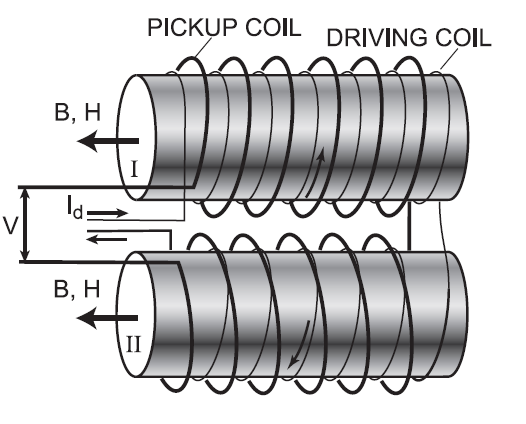
\includegraphics[width=0.50\textwidth]{schema}
\caption{Représentation d'un capteur recueillant une composante de l'espace tridimensionnel}
\end{center}
\end{figure}

L'enroulement des fils conducteurs sur les coeurs forment des bobines émettrices (chaque capteur à deux bobines émettrices). Ainsi, lorsque qu'un courant alternatif est appliqué aux fils conducteurs et que les capteurs sont positionnés dans un champ magnétique externe nul, ceux-ci émettent deux champs magnétiques (de même magnitude, mais de direction opposée, considérant l'enroulement du fil conducteur. La paire de bobine réceptrice est donc soumise à une variation de flux magnétique et la loi de Faraday nous indique que chacune de ces bobines obtient une force-électromotrice induite:
\[ \epsilon = -\frac{d \Phi}{dt} = -\frac{d}{dt} \iint_S  \vec{B}  \cdot \vec{dS}  \]  
Cependant, comme les champs magnétiques émis sont inversés et que les bobines réceptrices sont enroulées de la même façon la force-électromotrice induite totale est nulle (ne pas oublier que les capteurs sont dans un champ magnétique externe nul). Dans un autre ordre d'idée, les coeurs paramagnétiques, placées à l'intérieur des bobines émettrices, sont soumis à un champ magnétique émis variable ($\vec{H}$), ainsi les dipôles magnétiques à l'intérieur de ce matériau paramagnétique s'aligne avec la direction du champ magnétique ($\vec{H}$). Macroscopiquement, il y a présence d'une densité de flux variable ($\vec{B}$), à l'intérieur des coeurs, induit par le champ magnétique ($\vec{H}$). La relation graphique entre le champ magnétique $\vec{H}$ émis par les bobines et la densité de flux $\vec{B}$ à l'intérieur des coeurs est appelé une courbe d'hystérésis (voir figure x+1).  
  
\begin{figure}[h]
\begin{center}
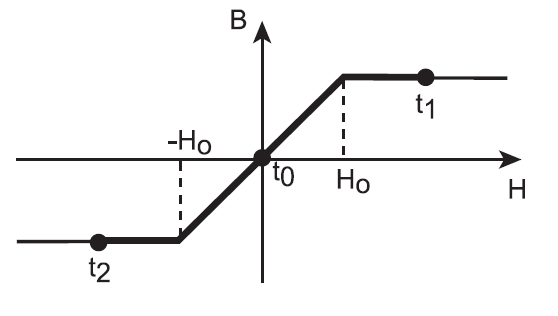
\includegraphics[width=0.50\textwidth]{hysteresis}
\caption{Courbe d'hystérésis idéalisée d'un matériau paramagnétique. Les domaines linéaires et constants sont symmétriques par rapport à l'origine.}
\end{center}
\end{figure}  

On pose l'hypothèse que le régime linéaire se situe entre $-H_o$ et $H_o$, puis que $||-H_o||=||H_o||$. Physiquement, les valeurs de $-H_o$ et $H_o$ sont  les valeurs de champ magnétique qui saturent l'aimantation des coeurs. Ainsi, lorsque l'on sort du régime linéaire $[-H_o;H_o]$, la densité de flux $\vec{B}$ est approximativement constante. Afin de bien représenter la force électromotrice induite, la loi de Faraday nous propose de trouver une représentation de $\vec{B}$ en fonction du temps. Jusqu'à présent, nous savons que $\vec{B} = \vec{B}(\vec{H}(t)) $. Cependant, chaque capteur travaille avec une composante de ces vecteurs, alors pour le besoin de la cause nous travaillerons avec les composantes de $\vec{B}$, telles que $B_i = B_i(H_i(t)$. Alors nous aurons trois composantes de force électromotrice induite:
\begin{equation}
\epsilon_i(t) = - \iint_S  \frac{\partial B_i(t)}{\partial dt}{dS_i}= -\pi r^2 \frac{\partial B_i(t)}{\partial t}   ,\ pour \ i=x,y,z 
\end{equation}
Par la suite, puisque $H_i(t)$ est produit à partir des bobines émettrices, cela  
nous permet d'avoir un certain contrôle sur la forme temporelle de $H_i(t)$ en fonction du temps, où $H_i(t)$ est péridique dans le temps, car la forme de $H_i(t)$ dépend directement de la forme d'onde du courant électrique injecté dans les bobines émettrices.
Après tout, nous voulons représenter $B_i(H_i(t))$, il faut donc combiner la fonction de $H_i(t)$ dans le temps et la courbe d'hystérésis qui met en relation $B_i$ et $H_i$. Il faut tout d'abord comprendre que le cycle d'héstérésis est parcouru entre les points $t_1$ à $t_2$ périodiquement. Comme $(B_i)$ est linéaire avec $(H_i)$ pour $[-H_o;H_o]$, les représentations graphique entre $B_i(t)$ et $H_i(t)$ dans le temps auront la même forme.  Par contre, lorsque l'on sort de la plage de linéarité $B_i(H(t))$ est approximativement une constante, ce qui veut dire que $H_i(t)$ peut continuer à varier dans le temps, lorsque $B_i(H(t))$ sature. Pour les besoins de l'explication, nous allons supposer que notre $H_i(t)$ est un signal triangulaire périodique. On peut alors bien visualiser la saturation de $B_i(t)$ à l'aide de la figure x+y.




\begin{figure}[h]
\begin{center}
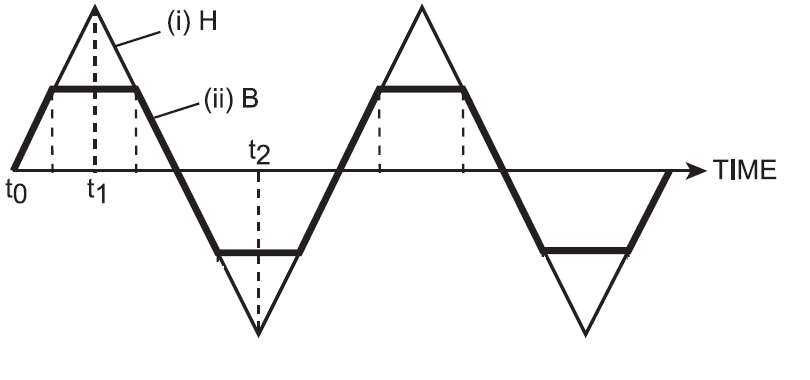
\includegraphics[width=0.50\textwidth]{saturation}
\caption{Représentation temporelle de $H_i(t)$ et de $B_i(t)$ dans le temps pour une onde de $H_i(t)$ triangulaire. On peut aussi implicitement visualiser la saturation de $B_i(t)$ les plages non-linéaires de la courbe d'hystérésis}
\end{center}
\end{figure} 




Dans l'exemple, les plages linéaires de la courbe d'hystérésis implique que le voltage induit est une constante, car $\frac{\partial B_i(t)}{\partial t} = c, \ $ et pour les plages saturées, le voltage induit est nul, car $\frac{\partial \vec{B}}{\partial t} = 0$. Ainsi, on peut s'attendre à avoir un signal périodique approximativement carré pour une bobine réceptrice. Comme les deux coeurs ont une densité de flux opposées, le voltage induit total est nul, car les deux signaux périodiques s'annulent (voir figure x+2). 

\begin{figure}[H]
\begin{center}
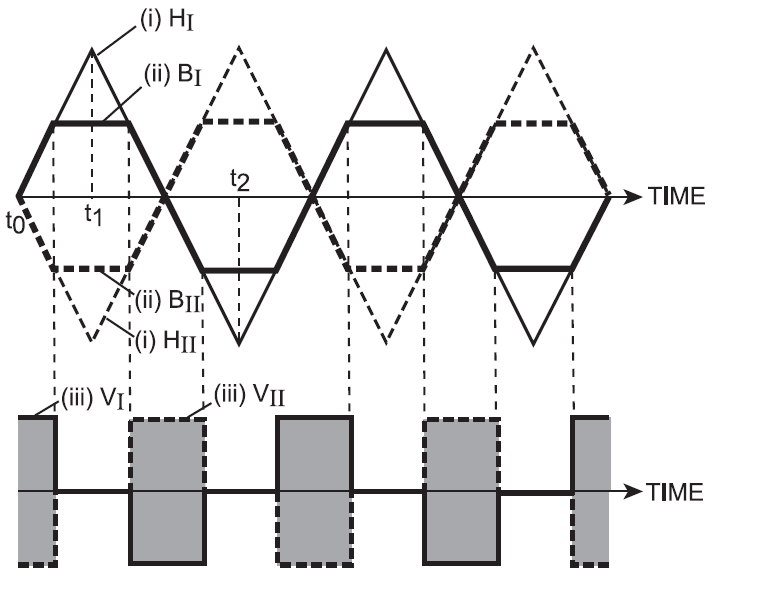
\includegraphics[width=0.50\textwidth]{voltage1}
\caption{$B_I$ représente le flux magnétique du premier coeur et $B_{II}$ le flux du second coeur. Comme les flux magnétiques sont opposés et que les bobines réceptrices sont du même sens, on retrouve un voltage induit nul.}
\end{center}
\end{figure} 

Notre voltage nul, tel que décrit ci-dessus est notre configuration de référence pour un champ externe nul. Pour obtenir cette configuration, il peut être nécessaire de placer le système dans une cage de Faraday, afin d'éviter que la mesure de référence soit perturbée par des facteurs externes non-voulues. Ensuite, en positionnant notre système activé (courant électrique alternatif) dans un champ magnétique externe constant, le cycle d'hystérésis n'est plus parcourue de manière symmétrique. La position moyenne du cycle n'est plus à l'origine, mais à un point $H_{ext}$ (voir figure 5), ce qui fait que les voltages induits sont translatés par rapport à la configuration nulle. En faisant des voltages induits dans les deux bobines réceptrices, on retrouve un voltage résiduel (voir figure).

\begin{figure}[H]
\begin{center}
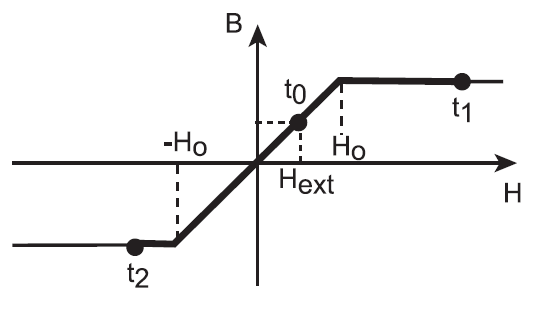
\includegraphics[width=0.50\textwidth]{hysteresis2}
\caption{figure 2 blabla}

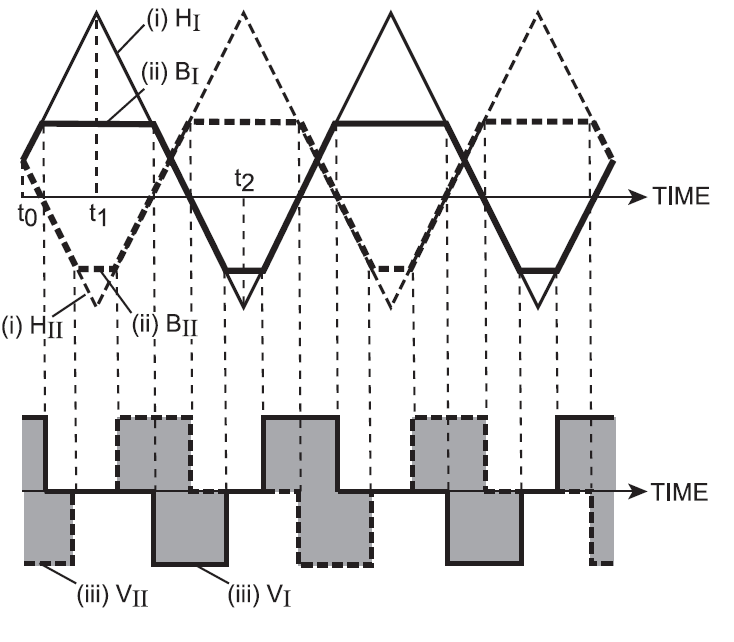
\includegraphics[width=0.50\textwidth]{voltage2}
\caption{figure 3 blabla}
\end{center}
\end{figure} 

Ce voltage induit résiduel additionné est proportionnel au champ magnétique externe (mettre référence). RAJOUTER BLABLA



\end{document}

\section{Solution sélectionnée}
\documentclass{standalone}
\usepackage[utf8]{inputenc}
%\usepackage[francais]{babel}
\usepackage[T1]{fontenc}
\usepackage{amsmath}
\usepackage{amsfonts}
\usepackage{amssymb}
\usepackage{graphicx}
\graphicspath{{/home/utilisateur1/Documents/Genie_physique/H2018/Projet_II/Magnetisme_projet}}%changer le numéro du devoir
\usepackage{standalone}
\usepackage{tikz}
\renewcommand{\thesection}{\arabic{section}}
\author{Bastien Gauthier-Soumis,\\
 Edward Halle-Hannan, ,\\
Massine Kadi, ,\\
Félix Pelletier, }
\begin{document}

\end{document}
\documentclass{standalone}
\usepackage[utf8]{inputenc}
%\usepackage[francais]{babel}
\usepackage[T1]{fontenc}
\usepackage{amsmath}
\usepackage{amsfonts}
\usepackage{amssymb}
\usepackage{graphicx}
\graphicspath{{/home/utilisateur1/Documents/Genie_physique/H2018/Projet_II/Magnetisme_projet}}%changer le numéro du devoir
\usepackage{standalone}
\usepackage{tikz}
\renewcommand{\thesection}{\arabic{section}}
\author{Bastien Gauthier-Soumis,\\
 Edward Halle-Hannan, ,\\
Massine Kadi, ,\\
Félix Pelletier, }
\begin{document}

\end{document}

\section{Discussion}
\documentclass{standalone}
\usepackage[utf8]{inputenc}
%\usepackage[francais]{babel}
\usepackage[T1]{fontenc}
\usepackage{amsmath}
\usepackage{amsfonts}
\usepackage{amssymb}
\usepackage{graphicx}
\graphicspath{{/home/utilisateur1/Documents/Genie_physique/H2018/Projet_II/Magnetisme_projet}}%changer le numéro du devoir
\usepackage{standalone}
\usepackage{tikz}
\renewcommand{\thesection}{\arabic{section}}
\author{Bastien Gauthier-Soumis,\\
 Edward Halle-Hannan, ,\\
Massine Kadi, ,\\
Félix Pelletier, }
\begin{document}
Le modèle employé pour décrire le fonctionnement d'un magnétomètre à saturation comporte certaines limites qui devront être prises en compte afin de guider la conception de l'instrument de mesure, le caractériser et analyser les données qui résulteront de son opération. Tout d'abord, la relation entre $\vert\vec{B}\vert=B$ et $\vert\vec{H}\vert=H$ utilisée est idéalisée et grandement approximative. On a considéré 
\begin{equation*}
\end{equation*}

\end{document}

\section{Références}
\documentclass{standalone}
\usepackage[utf8]{inputenc}
%\usepackage[francais]{babel}
\usepackage[T1]{fontenc}
\usepackage{amsmath}
\usepackage{amsfonts}
\usepackage{amssymb}
\usepackage{graphicx}
\graphicspath{{/home/utilisateur1/Documents/Genie_physique/H2018/Projet_II/Magnetisme_projet}}%changer le numéro du devoir
\usepackage{standalone}
\usepackage{tikz}
\renewcommand{\thesection}{\arabic{section}}
\author{Bastien Gauthier-Soumis,\\
 Edward Halle-Hannan, ,\\
Massine Kadi, ,\\
Félix Pelletier, }
\begin{document}

\end{document}

\end{document}